\documentclass[journal]{IEEEtran}

\usepackage{cite}
\usepackage{amsmath,amssymb,amsfonts}
\usepackage{graphicx}
\usepackage{textcomp}
\usepackage{subcaption}
\usepackage{booktabs}
\usepackage{multirow}
\usepackage{microtype}
\usepackage{caption}
\usepackage{balance}
\usepackage{algorithm}
\usepackage{algpseudocode}
\usepackage{siunitx}
\usepackage{url}
\captionsetup{font=small,labelfont=bf}
\captionsetup[table]{labelsep=colon, textfont=normalfont, labelfont=sc, font=footnotesize}

\graphicspath{{framework/}{representation/}{AW-DPCNN/}{MSCA-VGG16/}{Fused images/}{equipment/}{confusion_matrix/}{tsne/}{tsne_cwru/}{raw_tsne/}{tsne_models/}{figures/}}

\hyphenation{op-tical net-works semi-conduc-tor IEEE-Xplore}

\begin{document}

% \title{AW-DPCNN Based Multi-Representation Supervised Learning for Mechanical Signal Fault Diagnosis}
% \title{AW-DPCNN: Adaptive-Weighted Dual-PCNN Fusion of Time-Frequency Representations for Non-Stationary Fault Diagnosis}

% \title{Adaptive Multi-Representation Fusion with Multi-Scale Channel Attention for Vibration Signal Fault Diagnosis}
% \title{Adaptive Dual-Channel PCNN Multi-Representation Fusion and MSCA-VGG16 for Vibration Signal Fault Diagnosis}
% \title{Adaptive Weighted Dual-Channel Pulse-Coupled Neural Network Fusion with Multi-Scale Attention for Bearing Fault Diagnosis}
% \title{Adaptive Weighted Dual-Channel PCNN Multi-Representation Fusion with Multi-Scale Convolution for Vibration Signal Fault Diagnosis}
% \title{Adaptive Multi-Representation Fusion with Multi-Scale Convolution for Vibration Signal Fault Diagnosis}
% \title{Adaptive Multi-Representation Fusion of DPCNN with Multi-Scale Convolution for Vibration Signal Fault Diagnosis}
\title{Adaptive Multi-Representation Fusion via Dual-Channel PCNN with Multi-Scale Convolution for Vibration Signal Fault Diagnosis}

\author{Chen Yang, Zonglong Bai, Zhiyuan Xie, Chenggang Liu, Junyan Zhang and Yihe Guo
\thanks{This work is supported by the National Natural Science Foundation of
China (No. 12404545), Science Research Project of Hebei Education Department, China (No. QN2025334), and the Fundamental Research Funds for the
Central Universities (No. 2026MS144).}}


\markboth{IEEE Transactions on Instrumentation and Measurement}
{Yang~\MakeLowercase{\textit{et al.}}: AW-DPCNN Based Multi-Representation Supervised Learning for Mechanical Signal Fault Diagnosis}

\maketitle

\begin{abstract}
Vibration signal analysis is essential for the fault diagnosis of rotating machinery. However, existing methods based on single representations often fail to fully extract the discriminative features embedded in vibration signals. To address this single-representation limitation and adaptively fuse heterogeneous fault features, this paper proposes an adaptive weighted dual-channel pulse-coupled neural network (AW-DPCNN) for multi-representation fusion. The AW-DPCNN adaptively integrates complementary and heterogeneous short-time Fourier transform (STFT) spectrograms and Gramian angular difference field (GADF) images derived from vibration signals. Furthermore, to fully exploit the complementary information encoded in the fused representations, a multi-scale receptive fields and dynamic channel attention enhanced VGG16 (MSCA-VGG16) network is designed to improve fault diagnosis performance and noise robustness under lower signal-to-noise ratio conditions. Extensive experiments on the CWRU bearing dataset demonstrate that the proposed framework achieves 99.85\% accuracy on the 12~kHz drive-end benchmark, with strong cross-sensor generalization (97.45\% on fan-end data) and cross-sampling-rate robustness (94.81\% at 48~kHz). Ablation studies confirm that adaptive weighting contributes 2.93\% and multi-scale convolution adds 0.54\% over the respective baselines, while noise robustness tests validate stable performance under degraded signal conditions.
\end{abstract}

\begin{IEEEkeywords}
Fault diagnosis, Gramian angular difference field (GADF), pulse coupled neural network (PCNN), short-time Fourier transform (STFT), vibration signal.
\end{IEEEkeywords}

\section{Introduction}
\IEEEPARstart{R}{otating} machinery, including bearings, gears, and shafts, constitutes the core of modern industrial systems~\cite{10313245},~\cite{GAO2026114419}. Unexpected failures of these critical components can lead to catastrophic breakdowns, substantial economic losses, and severe safety hazards. Consequently, reliable and intelligent fault diagnosis techniques have become indispensable for condition-based maintenance and operational safety assurance~\cite{6899683}. Among various diagnostic modalities, vibration-based monitoring has received the most extensive research attention due to its rich fault-related information content, non-intrusive sensor deployment, and well-established physical understanding of fault-induced vibration signatures~\cite{YI2025116881},~\cite{9440949}.

Despite the practical success of vibration-based diagnosis, the non-stationary nature of real-world machinery signals remains a fundamental challenge. Under variable speed, fluctuating load, and time-varying operating conditions, vibration signals exhibit pronounced non-stationary characteristics, as their spectral content and statistical properties evolve over time in complex ways that cannot be adequately captured by conventional stationary signal processing techniques~\cite{8853278}~\cite{9242332}. Single time-domain or frequency-domain representations each capture only partial aspects of these rich signals. Time-domain features may overlook critical spectral information, while frequency-domain representations discard temporal evolution patterns that are essential for distinguishing transient fault events from steady-state operating conditions~\cite{HONG20142164}~\cite{10319398}.

To address the limitations of single-representation approaches, researchers have explored complementary representation strategies. Time--frequency representations such as the short-time Fourier transform (STFT) spectrogram, Mel spectrogram, and continuous wavelet transform (CWT) scalogram provide joint time--frequency energy distributions that reveal how spectral content evolves temporally~\cite{10226588},~\cite{DONG2023108934},~\cite{10659159}. In parallel, temporal encoding methods such as the Gramian Angular Field (GAF), Markov transition field (MTF), and recurrence plot (RP) transform one-dimensional time series into two-dimensional images by encoding pairwise temporal relationships, thereby preserving global temporal correlation structures that time--frequency methods may not explicitly capture~\cite{ZHANG2026106301},~\cite{10517915}~\cite{LIU20254863}. However, most existing studies adopt a single representation for downstream classification, and the complementary nature of time--frequency and temporal-encoded representations remains largely underexploited.

Multi-representation fusion offers a natural avenue to combine the strengths of heterogeneous representations, while existing fusion strategies face critical limitations. Simple concatenation or pixel-wise averaging ignores the distinct statistical properties and structural characteristics of different representations, potentially introducing destructive interference rather than constructive complementarity~\cite{8513874}~\cite{10260234}. Fixed-weight fusion schemes lack the adaptivity to emphasize discriminative representations while suppressing less informative ones on a per-sample or per-region basis~\cite{PENG2012164}. Furthermore, conventional deep learning classifiers are typically optimized for single-representation inputs and lack dedicated architectural mechanisms for capturing the multi-scale and channel-wise characteristics that emerge from multi-representation fusion~\cite{11345448}~\cite{8788665}.

To address these gaps, this paper proposes a two-stage framework comprising an adaptive weighted dual-branch pulse-coupled neural network (AW-DPCNN) for multi-representation fusion, and a multi-scale channel attention enhanced VGG16 (MSCA-VGG16) classifier for robust fault identification. The main contributions are summarized as follows.

\begin{itemize}
\item An AW-DPCNN fusion mechanism is proposed to adaptively integrate STFT spectrograms and Gramian angular difference field (GADF) images. The mechanism introduces contrast-guided adaptive weighting to dynamically regulate per-channel contributions, dual-channel external stimuli with representation-specific convolutional kernels, and iterative pulse-coupled dynamics for feature reinforcement.

\item An MSCA-VGG16 classification network is constructed to further exploit the complementary information encoded in the fused representations. The architecture integrates multi-scale convolution for capturing fault patterns at multiple temporal and spectral granularities, squeeze-and-excitation channel attention for dynamic frequency-band recalibration, and a compact embedding head for enhanced discriminability.

% \item Extensive experiments on the CWRU bearing dataset, including backbone comparisons, comprehensive ablation studies, representation comparisons across twelve time--frequency and temporal encoding combinations, noise robustness evaluations, and hyperparameter sensitivity analyses, systematically validate each component of the proposed framework. Cross-sensor and cross-sampling-rate generalization is further demonstrated on the 12 kHz fan-end and 48 kHz drive-end datasets, confirming robustness beyond the primary benchmark.
\item Extensive experiments on the CWRU bearing dataset, including backbone comparisons, ablation studies, representation comparisons, and noise robustness evaluations, validate the proposed framework. Cross-sensor and cross-sampling-rate generalization is further demonstrated on the 12 kHz fan-end and 48 kHz drive-end datasets.

\end{itemize}

The remainder of this paper is organized as follows. Section~\ref{section2} reviews related work. Section~\ref{section3} presents the proposed AW-DPCNN fusion mechanism and MSCA-VGG16 classifier. Section~\ref{section4} describes the experimental setup and comprehensive performance evaluation. Finally, conclusions are drawn in Section~\ref{section5}.
\begin{figure*}[!t]
\centering
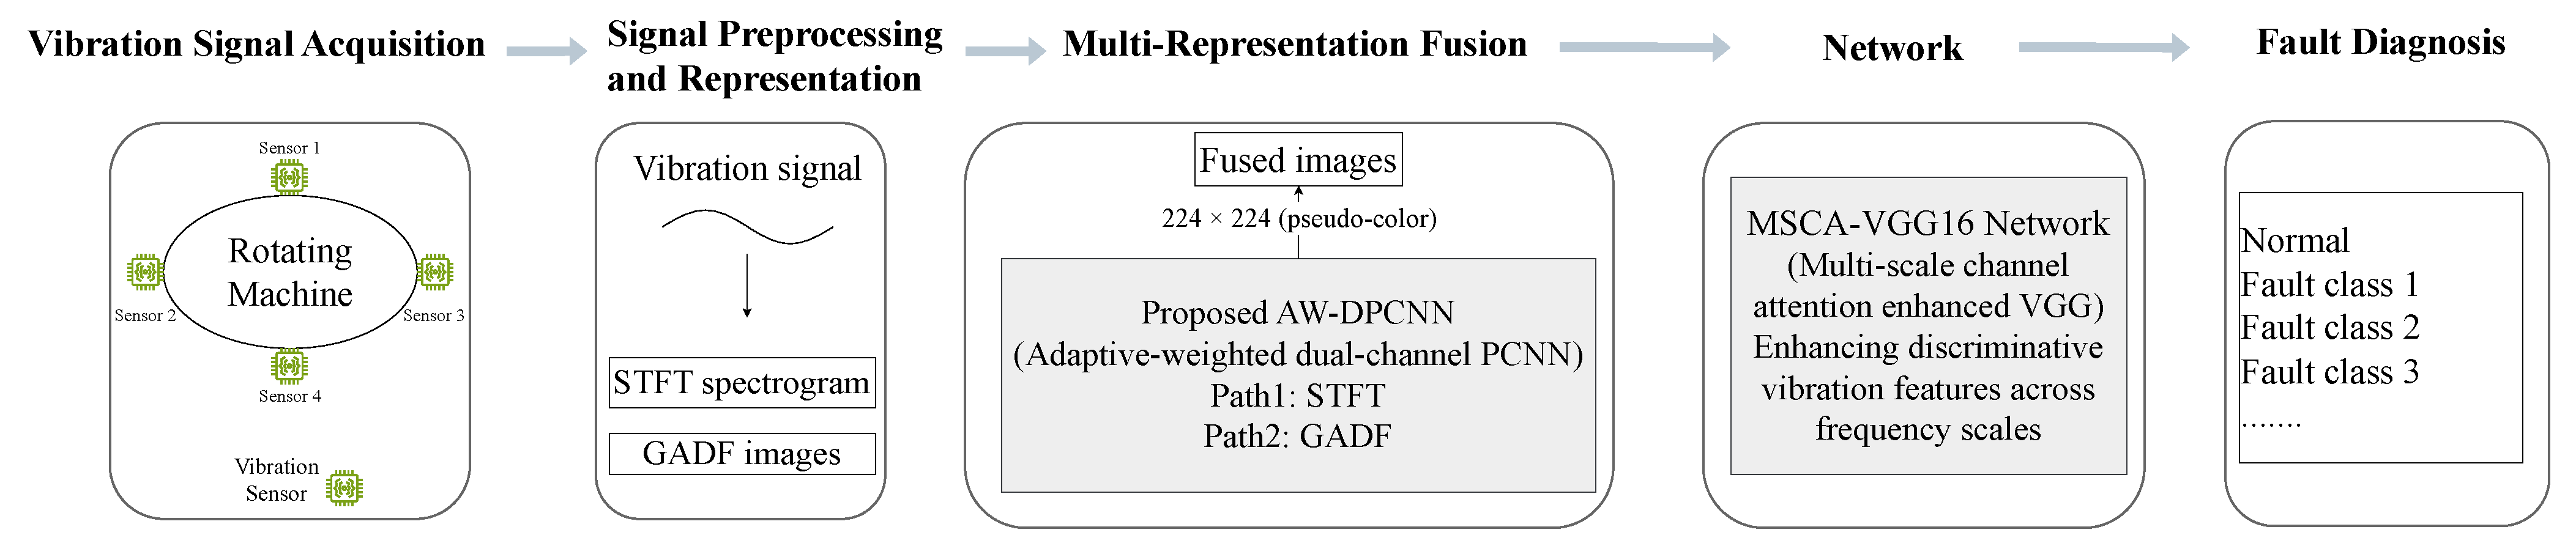
\includegraphics[width=\linewidth]{framework/framework1}
\caption{Overall framework of the proposed vibration signal fault diagnosis method. The vibration signal is first converted into STFT spectrograms and GADF images. These heterogeneous representations are then adaptively fused through the proposed AW-DPCNN mechanism. Finally, the fused features are fed into the MSCA-VGG16 network for fault classification.}
\label{framework}
\end{figure*}

\section{Related Work}
\label{section2}

\subsection{Signal Representations for Fault Diagnosis}

Time--frequency representations have been extensively applied to vibration-based
bearing fault diagnosis, such as STFT spectrograms, CWT scalograms, and Mel spectrograms. STFT spectrograms combined with 2-D CNNs have demonstrated
effective classification of bearing defects by converting raw vibration signals into
time--frequency images that convolutional architectures can process~\cite{11028059},
\cite{Xin_2019}. CWT scalograms have been employed to achieve improved time--frequency
localization for transient fault signatures, with multi-resolution analysis offering
advantages over fixed-resolution STFT for certain non-stationary conditions~\cite{SHAALAN2026103187}.
Mel spectrograms have also been explored for their perceptually motivated frequency
compression, particularly for harmonic-rich fault patterns~\cite{10929672}. Despite
these successes, time--frequency representations inherently capture local
spectral energy distributions but do not explicitly model the long-range temporal
dependencies that carry complementary diagnostic information.

In parallel, temporal encoding methods have been introduced to transform
one-dimensional vibration signals into two-dimensional images that preserve pairwise
temporal relationships. Xiong et al. applied GAF encoding to complementary ensemble empirical mode decomposition-preprocessed vibration signals, enabling CNN-based classification of the resulting temporal correlation images~\cite{10109681}. MTF and RP encodings have similarly been adopted to
capture sequential transition dynamics and recurrent phase-space patterns,
respectively~\cite{11303191},~\cite{10684078}. However, these temporal encoding methods primarily preserve correlation
structures and lack explicit frequency-domain specificity, which is critical for
distinguishing faults with similar temporal patterns but distinct spectral signatures.

A limited number of recent studies have explored combining multiple representations
for fault diagnosis. Representative efforts include channel-wise concatenation of
time--frequency and temporal-encoded images for CNN-based classification, and
pixel-level averaging of complementary representation pairs~\cite{10214203}. However, these approaches
employ fixed fusion strategies that treat all spatial locations and feature channels
uniformly, without adaptively regulating the relative contribution of each
representation. Given that time--frequency and temporal-encoded representations
possess fundamentally different statistical properties and structural characteristics,
naive fusion may introduce destructive interference rather than constructive
complementarity.

\subsection{PCNN and Multi-Representation Fusion}
Pulse-coupled neural network (PCNN) is a neural model originally developed to simulate the synchronous firing behavior observed in the mammalian visual cortex \cite{761706}. Unlike conventional convolutional neural networks, PCNN employs a pulse-based activation mechanism in which neurons interact through local coupling and dynamic thresholds \cite{761716}. Owing to these characteristics, PCNN exhibits strong capability in preserving structural information while suppressing background interference, and have been widely applied in image segmentation, edge detection, and feature enhancement tasks~\cite{1427771},~\cite{Deng_2020},~\cite{Liu_2019}. 

However, conventional PCNNs are typically driven by a single external stimulus, which limits their ability to effectively exploit complementary information from multiple representations. To address this limitation, dual-channel PCNN (DPCNN) architectures have been introduced to enable multi-representation fusion by incorporating multiple external stimuli within the neuronal feeding mechanism, and later extended with adaptive parameter estimation via fractal dimension to eliminate manual tuning~\cite{9072551}. Through this mechanism, heterogeneous feature maps can be jointly processed, thereby facilitating the integration of information from different representations. Nevertheless, the fusion process in such architectures generally relies on fixed or predefined coupling strategies, making it difficult to adaptively regulate the relative contributions of different channels. As a result, the model may not effectively emphasize discriminative representations while suppressing less relevant ones, thereby limiting the effectiveness of multi-representation fusion. The systematic exploration and adaptive fusion of heterogeneous representations for vibration signal fault diagnosis therefore remains an open research problem, motivating the AW-DPCNN framework proposed in this work.

\subsection{Deep Learning for Fault Diagnosis}

With the rapid advancement of deep learning techniques, a variety of neural network architectures have been applied to vibration signal fault diagnosis, demonstrating superior automatic feature extraction capability compared with traditional handcrafted methods~\cite{JIANG2026113823},~\cite{COSTA2026113711}. Early studies commonly adopted baseline convolutional neural networks as benchmark architectures for vibration signal fault diagnosis, verifying the feasibility of end-to-end feature learning for fault diagnosis tasks \cite{HE2020542}. Subsequently, classical deep convolutional backbones, including EfficientNet, ViT, MobileNet, ConvNeXt and ResNet, were introduced into intelligent fault diagnosis frameworks and achieved notable improvements in hierarchical feature representation and classification accuracy across machinery health monitoring applications~\cite{10663388},~\cite{DUAN2026122469},~\cite{10048773}. Among these, VGG's purely sequential topology with no skip connections or built-in attention mechanisms provides a clean architectural foundation for attaching auxiliary modules such as multi-scale convolution and channel attention, making it particularly suitable as a backbone for the MSCA enhancement strategy pursued in this work~\cite{WANG2026105996}. More recently, advanced architectures such as ConvNeXt, which incorporate modernized convolutional design principles, have further enhanced representation learning capability and demonstrated competitive performance in fault diagnosis and image-based classification tasks~\cite{10980179}. In addition, publicly available benchmark datasets, such as the CWRU bearing fault dataset, have been extensively employed to evaluate the effectiveness and generalization ability of deep learning-based diagnostic models, serving as a standard reference in fault diagnosis research \cite{SMITH2015100}.

Despite these advances, most existing deep learning approaches for fault diagnosis are designed to process a single input representation and lack dedicated architectural mechanisms, such as multi-scale receptive fields and dynamic channel attention, for jointly exploiting the heterogeneous features produced by multi-representation fusion. Consequently, their capacity to fully leverage the complementary information encoded in fused time--frequency and temporal representations remains limited, motivating the design of the MSCA-VGG16 classifier proposed in this work.

\section{Methodology}
\label{section3}

\subsection{Overview}
The proposed framework comprises two sequential stages, i.e., multi-representation signal fusion and fused representation classification, as illustrated in Fig.~\ref{framework}. In the fusion stage, the raw vibration signal is first transformed into two complementary representations, namely the STFT spectrogram and the GADF image, to capture time--frequency energy distributions and global temporal correlation structures, respectively. These heterogeneous representations are then adaptively integrated through the proposed AW-DPCNN mechanism, which employs contrast-guided adaptive weighting and dual-channel pulse-coupled dynamics to produce a unified fused representation. In the classification stage, the fused representation is fed into the MSCA-VGG16 network, which incorporates multi-scale convolution and channel attention to enhance feature discrimination, followed by a compact embedding head for robust fault classification.

Let $\boldsymbol{x} \in \mathbb{R}^{L}$ denote a raw vibration signal segment of length $L$. The signal is first mapped to two heterogeneous representations as
\begin{equation}
\boldsymbol{S}_{\mathrm{STFT}} = \mathcal{T}_{\mathrm{STFT}}(\boldsymbol{x}), \quad
\boldsymbol{S}_{\mathrm{GADF}} = \mathcal{T}_{\mathrm{GADF}}(\boldsymbol{x}),
\label{eq:pipeline_rep}
\end{equation}
where $\mathcal{T}_{\mathrm{STFT}}(\cdot)$ and $\mathcal{T}_{\mathrm{GADF}}(\cdot)$ denote the STFT and GADF operators, respectively. The two representations are then fused via the AW-DPCNN operator $\mathcal{F}_{\mathrm{AW}}(\cdot, \cdot)$ as
\begin{equation}
\boldsymbol{S}_{\mathrm{fused}} = \mathcal{F}_{\mathrm{AW}}(\boldsymbol{S}_{\mathrm{STFT}}, \boldsymbol{S}_{\mathrm{GADF}}; \Theta_{\mathrm{AW}}),
\label{eq:pipeline_fuse}
\end{equation}
where $\Theta_{\mathrm{AW}}$ denotes the set of AW-DPCNN hyperparameters. Finally, the fused representation is passed through the MSCA-VGG16 classifier $\mathcal{C}(\cdot)$ to produce the predicted fault class probabilities
\begin{equation}
\hat{\boldsymbol{y}} = \mathcal{C}(\boldsymbol{S}_{\mathrm{fused}}; \Theta_{\mathrm{CLS}}),
\label{eq:pipeline_cls}
\end{equation}
where $\Theta_{\mathrm{CLS}}$ denotes the trainable parameters of the classification network and $\hat{\boldsymbol{y}} \in \mathbb{R}^{K}$ is the predicted probability vector over $K$ fault categories. The following subsections detail each component of this pipeline.

\subsection{Signal Representation}

The raw vibration signal segment $\boldsymbol{x} \in \mathbb{R}^{L}$, introduced in~\eqref{eq:pipeline_rep}, serves as the common input from which both representations are derived. The STFT spectrogram $\boldsymbol{S}_{\mathrm{STFT}}$ captures local time--frequency energy distributions through short-time spectral analysis, while the GADF image $\boldsymbol{S}_{\mathrm{GADF}}$ encodes global temporal correlation structures through pairwise angular relationships. Their respective constructions are detailed below.

\subsubsection{STFT Spectrogram}

The STFT spectrogram is a linear time--frequency representation that preserves uniform frequency resolution across the entire spectrum. Let $x[k]$ denote the $k$-th sample of the vibration signal segment $\boldsymbol{x}$. The construction involves dividing $\boldsymbol{x}$ into overlapping frames of length $n_{\mathrm{fft}}$, applying a Hann window $w(\cdot)$ to each frame, and computing the discrete Fourier transform. The magnitude spectrum of each frame is arranged chronologically to form a two-dimensional time--frequency representation $\boldsymbol{S}_{\mathrm{STFT}}(t, f)$, defined as
\begin{equation}
\boldsymbol{S}_{\mathrm{STFT}}(t, f) = \left| \sum_{k=0}^{n_{\mathrm{fft}}-1} x[k] \, w(k - t) \, e^{-j 2\pi f k / n_{\mathrm{fft}}} \right|^2.
\label{eq:stft}
\end{equation}

The STFT spectrogram is parameterized by the FFT window size $n_{\mathrm{fft}}$ and hop length, which jointly determine the temporal resolution and frequency resolution $\Delta f = f_s / n_{\mathrm{fft}}$ at a given sampling rate $f_s$.

\begin{figure}[!t]
	\centering
	\graphicspath{{representation/}}
	\begin{subfigure}{0.48\linewidth}
		\centering
		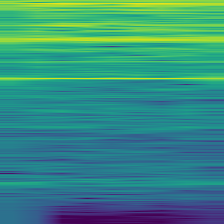
\includegraphics[width=\linewidth]{STFT_98_Normal_1_00000}
		\caption{STFT spectrogram}
	\end{subfigure}
	\hfill
	\begin{subfigure}{0.48\linewidth}
		\centering
		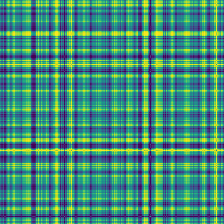
\includegraphics[width=\linewidth]{GADF_98_Normal_1_00000}
		\caption{GADF image}
	\end{subfigure}
	
	\caption{Vibration signal representations. (a) STFT spectrogram capturing local time--frequency energy distributions. (b) GADF image encoding global temporal correlation structures through pairwise angular relationships.}
	\label{representation}
	
\end{figure}

\subsubsection{Gramian Angular Field}

% To address the limitations of the STFT spectrogram in encoding global temporal structures, the Gramian Angular Field (GAF) is introduced as a complementary representation. 
The GAF transforms the same vibration signal segment $\boldsymbol{x}$ into a two-dimensional image that preserves temporal correlation information through pairwise angular encoding. Let $x_i$ denote the $i$-th sample of $\boldsymbol{x}$. For the purpose of GADF construction, a sequence of $n$ samples $\{x_1, x_2, \ldots, x_n\}$ drawn from $\boldsymbol{x}$ is first normalized to $[-1, 1]$ via min--max scaling,
% \begin{equation}
% \tilde{x}_i = \frac{\bigl(x_i - \min\limits_{i\in I} \boldsymbol{x_i}\bigr) + \bigl(x_i - \max\limits_{i\in I}\boldsymbol{x_i}\bigr)}
% {\max\limits_{i\in I}\boldsymbol{x_i} - \min\limits_{i\in I}\boldsymbol{x_i}},
% \label{normalization}
% \end{equation}
\begin{equation}
\tilde{x}_i = \frac{\left(x_i - \min\limits_{i\in I} x_i\right) + \left(x_i - \max\limits_{i\in I} x_i\right)}
{\max\limits_{i\in I} x_i - \min\limits_{i\in I} x_i},
\label{eq:normalization}
\end{equation}
where $I = \{1, 2, \ldots, n\}$ denotes the index set of the selected samples, and $\min\limits_{i\in I} x_i$ and $\max\limits_{i\in I} x_i$ are the minimum and maximum values of the sequence $\{x_i\}_{i=1}^n$, respectively.
% \begin{equation}
% \tilde{x}_i = \frac{(x_i - \min\boldsymbol{x_i}) + (x_i - \max\boldsymbol{x_i})}
% {\max\boldsymbol{x_i} - \min\boldsymbol{x_i}}.
% \label{normalization}
% \end{equation}

The normalized values are then mapped to polar coordinates, where each $\tilde{x}_i$ is encoded as an angular coordinate $\phi_i$,
\begin{equation}
\phi_i = \arccos(\tilde{x}_i), -1 \leq \tilde{x}_i \leq 1
\label{eq:cosine_angle}
\end{equation}

Finally, pairwise angular differences or sums are aggregated to form the Gramian Angular Summation Field (GASF) and GADF. The GADF variant,
\begin{equation}
\boldsymbol{G_d}(i,j) = \sin(\phi_i - \phi_j), \quad i,j = 1,\ldots,n,
\label{eq:gadf}
\end{equation}
is adopted in this study due to its higher sensitivity to abrupt temporal variations.

The GADF representation offers several advantages that complement the STFT spectrogram. First, by encoding pairwise angular relationships between all time points, the GADF captures global temporal correlation structures that extend beyond the local receptive field of STFT-based representations. Second, the min--max normalization in~\eqref{eq:normalization} inherently suppresses the influence of absolute signal amplitude, making the GADF representation more robust to variations in signal gain and background noise levels. Furthermore, the polar encoding in~\eqref{eq:cosine_angle} provides a bijective mapping, ensuring that temporal information is preserved without loss. 
% As illustrated in Fig.~\ref{representation}(b), the GADF encodes structured temporal dependencies, exhibiting regular and symmetric patterns that reflect stable temporal correlations.

Both representations are subsequently converted to pseudo-color RGB images of spatial dimensions $H \times W$ for compatibility with standard CNN input architectures, through logarithmic amplitude compression and colormap mapping. Fig.~\ref{representation} illustrates representative examples of the STFT spectrogram and GADF image. The concrete parameter values, including $n_{\mathrm{fft}}$, $f_s$, $n$, $H$, and $W$, are provided in Section~\ref{sec:dataset_preprocessing}.

% In this study, the GADF variant is specifically adopted to complement the STFT spectrogram. Compared with GASF, GADF focuses on angular differences and thereby exhibits higher sensitivity to abrupt temporal variations and asymmetric dynamic patterns. This property is particularly beneficial for bearing fault diagnosis, where abnormal operating conditions produce irregular temporal fluctuations in vibration signals. 



\subsection{AW-DPCNN for Multi-Representation Fusion}
\label{sec:awdpcnn}

Owing to their distinct statistical properties and structural characteristics, directly combining the STFT spectrogram and GADF image using conventional pixel-wise averaging or simple feature concatenation may introduce destructive interference rather than constructive complementarity, as demonstrated in the ablation study (Section~\ref{section4}). To address this issue, the proposed AW-DPCNN introduces a PCNN-inspired fusion mechanism with three key innovations: (i) dual-channel external stimuli that independently process STFT and GADF representations through representation-specific convolutional kernels; (ii) a contrast-guided adaptive weighting scheme that dynamically adjusts the relative contribution of each representation based on local saliency; and (iii) iterative pulse-coupled dynamics that propagate and reinforce structurally consistent features across multiple iterations while suppressing spurious activations. The key hyperparameters of the AW-DPCNN are summarized in Table~\ref{tab:awdpcnn_params}, and the detailed formulation of each component is presented below.

\begin{table}[!t]
	\caption{Key Hyperparameters of AW-DPCNN, where $\text{I}$ Denotes the Identity Matrix\label{tab:awdpcnn_params}}
	\centering
	\begin{tabular}{ccc}
		\hline
		\textbf{Parameter} & \textbf{Symbol} & \textbf{Value} \\
		\hline
		Iteration number & $N$ & 20 \\
		Decay coefficient & $\alpha_L$ & 0.001 \\
		Threshold decay & $\alpha_T$ & 0.001 \\
		Amplification coefficient & $V_T$ & 20 \\
		Stabilization constant & $\sigma$ & 0.1 \\
		Contrast amplification factor & $\gamma$ & 10 \\
		Local neighborhood window size & $\boldsymbol{\Omega}$ & $3 \times 3$ \\
		Kernel size of STFT channel & $\boldsymbol{W}_1$ & $3 \times 5$ \\
		Kernel size of GADF channel & $\boldsymbol{W}_2$ & $3 \times 3$ \\
		Coupling matrix & $\boldsymbol{M}$ & $$0.25\,\text{I}$$ \\
		\hline
	\end{tabular}
\end{table}

\subsubsection{Input Normalization}
To eliminate scale differences between two representations, each input is first normalized to the interval $[0,1]$ as
% \begin{equation}
% 	\boldsymbol{\tilde{S}}_k(i,j) = \frac{\boldsymbol{S}_k(i,j) - \min\boldsymbol{S}_k}{\max\boldsymbol{S}_k - \min\boldsymbol{S}_k + \epsilon}, \quad k\in\{1,2\}
% 	\label{eq:aw_input_norm}
% \end{equation}

\begin{equation}
	\boldsymbol{\tilde{S}}_k(i,j) = \frac{\boldsymbol{S}_k(i,j) - \min\limits_{i\in I,j\in J} \boldsymbol{S}_k(i,j)}{\max\limits_{i\in I,j\in J} \boldsymbol{S}_k(i,j) - \min\limits_{i\in I,j\in J} \boldsymbol{S}_k(i,j) + \epsilon}, \quad k\in\{1,2\}
	\label{eq:aw_input_norm}
\end{equation}
% \begin{equation}
% 	\boldsymbol{\tilde{S}}_k(i,j) = \frac{\boldsymbol{S}_k(i,j) - \min\limits_{\substack{i\in I\\ j\in J}} \boldsymbol{S}_k(i,j)}{\max\limits_{\substack{i\in I\\ j\in J}} \boldsymbol{S}_k(i,j) - \min\limits_{\substack{i\in I\\ j\in J}} \boldsymbol{S}_k(i,j) + \varepsilon}, \quad \text{for } k=1,2
% 	\label{eq:aw_input_norm}
% \end{equation}
where $\boldsymbol{S}_1$ and $\boldsymbol{S}_2$ denote the STFT spectrogram and GADF image, respectively, and $\epsilon$ is a small positive constant.

\subsubsection{Contrast-Guided Adaptive Weighting}
For each representation, the local mean of the normalized representation is computed as
\begin{equation}
	\boldsymbol{\mu}_k(i,j) = \frac{1}{|\boldsymbol{\Omega}|}
	\sum_{(p,q)\in \boldsymbol{\Omega}} \boldsymbol{\tilde{S}}_k(p,q),
	\label{eq:local_mean}
\end{equation}
where $\boldsymbol{\Omega}$ denotes the local neighborhood centered at each pixel location, and $|\boldsymbol{\Omega}|$ represents the number of elements in the neighborhood.

The corresponding local contrast is defined as the local standard deviation
\begin{equation}
	C_k(i,j) = \sqrt{ \left| \mathbb{E}_\Omega \left[ \tilde{S}_k^2 \right] - \mu_k^2(i,j) \right| },
	\label{eq:local_contrast}
\end{equation}
where $\mathbb{E}_\Omega[\cdot]$ denotes local averaging within $\boldsymbol{\Omega}$. A contrast amplification factor $\gamma$ is then introduced to construct adaptive fusion weights
\begin{equation}
	\beta_1(i,j) = 
	\frac{\gamma C_1(i,j)}
	{\gamma C_1(i,j) + C_2(i,j) + \epsilon},
	\label{eq:beta1}
\end{equation}
\begin{equation}
	\beta_2(i,j) = 
	\frac{C_2(i,j)}
	{\gamma C_1(i,j) + C_2(i,j) + \epsilon},
	\label{eq:beta2}
\end{equation}
the above formulation ensures $\beta_1(i,j) + \beta_2(i,j) \approx 1$, enabling contrast-driven dynamic weighting.

\subsubsection{Dual-Channel PCNN}
Let $\boldsymbol{L}^n(i,j)$, $\boldsymbol{T}^n(i,j)$, and $\boldsymbol{Y}^n(i,j)$ denote the linking term, dynamic threshold, and binary pulse output, respectively, where $n$ denotes the current iteration and $n \in [1, N]$, with $N$ being the total number of iterations. The neural states are initialized as
\begin{equation}
	\boldsymbol{L}^0(i,j) = \boldsymbol {0}, \quad 
	\boldsymbol{T}^0(i,j) = \boldsymbol {0}, \quad 
	\boldsymbol{Y}^0(i,j) = \boldsymbol {0}.
	\label{eq:initialization}
\end{equation}

At the $n$-th iteration, the external stimulus from two channels is defined as
\begin{equation}
	\boldsymbol{F}_1^n(i,j) = (\boldsymbol{W}_1 * \boldsymbol{Y}^{n-1})(i,j) + \boldsymbol{\tilde{S}}_1(i,j)
	\label{eq:f1_update}
\end{equation}
\begin{equation}
	\boldsymbol{F}_2^n(i,j) = (\boldsymbol{W}_2 * \boldsymbol{Y}^{n-1})(i,j) + \boldsymbol{\tilde{S}}_2(i,j),
	\label{eq:f2_update}
\end{equation}
where $\boldsymbol{W}_1$ and $\boldsymbol{W}_2$ are representation-specific convolutional kernels, i.e., stripe-shaped kernels for the STFT channel to emphasize frequency continuity, and symmetric kernels for the GADF channel to capture temporal correlations. Besides, $*$ denotes convolution.

The internal linking state is updated by
\begin{equation}
	\boldsymbol{L}^n(i,j) = e^{-\alpha_L} \boldsymbol{L}^{n-1}(i,j) + (\boldsymbol{M} * \boldsymbol{Y}^{n-1})(i,j),
	\label{eq:linking_update}
\end{equation}
where $\alpha_L$ is the decay coefficient and $\boldsymbol M$ represents the coupling matrix.

The total neuron input is then given by
\begin{equation}
	\boldsymbol{U}^n(i,j) = \big(1 + \boldsymbol{L}^n(i,j)\big)\Big(1 + \beta_1 \boldsymbol{F}_1^n(i,j)\Big)
	\Big(1 + \beta_2 \boldsymbol{F}_2^n(i,j)\Big) + \sigma,
	\label{eq:internal_activity}
\end{equation}
where $\sigma$ is a stabilization constant.

The pulse output is determined by a threshold comparison as follows
\begin{equation}
	\boldsymbol{Y}^n(i,j) =
	\begin{cases}
		1, & \boldsymbol{U}^n(i,j) > \boldsymbol{T}^{n-1}(i,j) \\
		0, & \text{otherwise}
	\end{cases}.
	\label{eq:pulse_output}
\end{equation}

The dynamic threshold evolves according to
\begin{equation}
	\boldsymbol{T}^n(i,j) = e^{-\alpha_T} \boldsymbol{T}^{n-1}(i,j) + V_T \boldsymbol{Y}^n(i,j),
	\label{eq:threshold_update}
\end{equation}
where $\alpha_T$ controls threshold decay and $V_T$ is the amplification coefficient.

\subsubsection{Fused Representation}
The accumulated neural response after $N$ iterations is
\begin{equation}
	\boldsymbol{U}_{\mathrm{sum}}(i,j)=\sum_{n=1}^{N} \boldsymbol{U}^{n}(i,j),
\end{equation}
and the final fused representation is obtained via normalization as
\begin{equation}
	\boldsymbol{F}(i,j)=
	\frac{\boldsymbol{U}_{\mathrm{sum}}(i,j)-\min\limits_{i,j} \boldsymbol{U}_{\mathrm{sum}}(i,j)}
	{\max\limits_{i,j} \boldsymbol{U}_{\mathrm{sum}}(i,j)-\min\limits_{i,j} \boldsymbol{U}_{\mathrm{sum}}(i,j)+\epsilon}.
\end{equation}

The overall architecture of the proposed AW-DPCNN is illustrated in Fig.~\ref{AW-DPCNN}. The qualitative effectiveness of the adaptive fusion mechanism is further analyzed in Section~\ref{section4}.
\begin{figure}[!t]
	\centering
	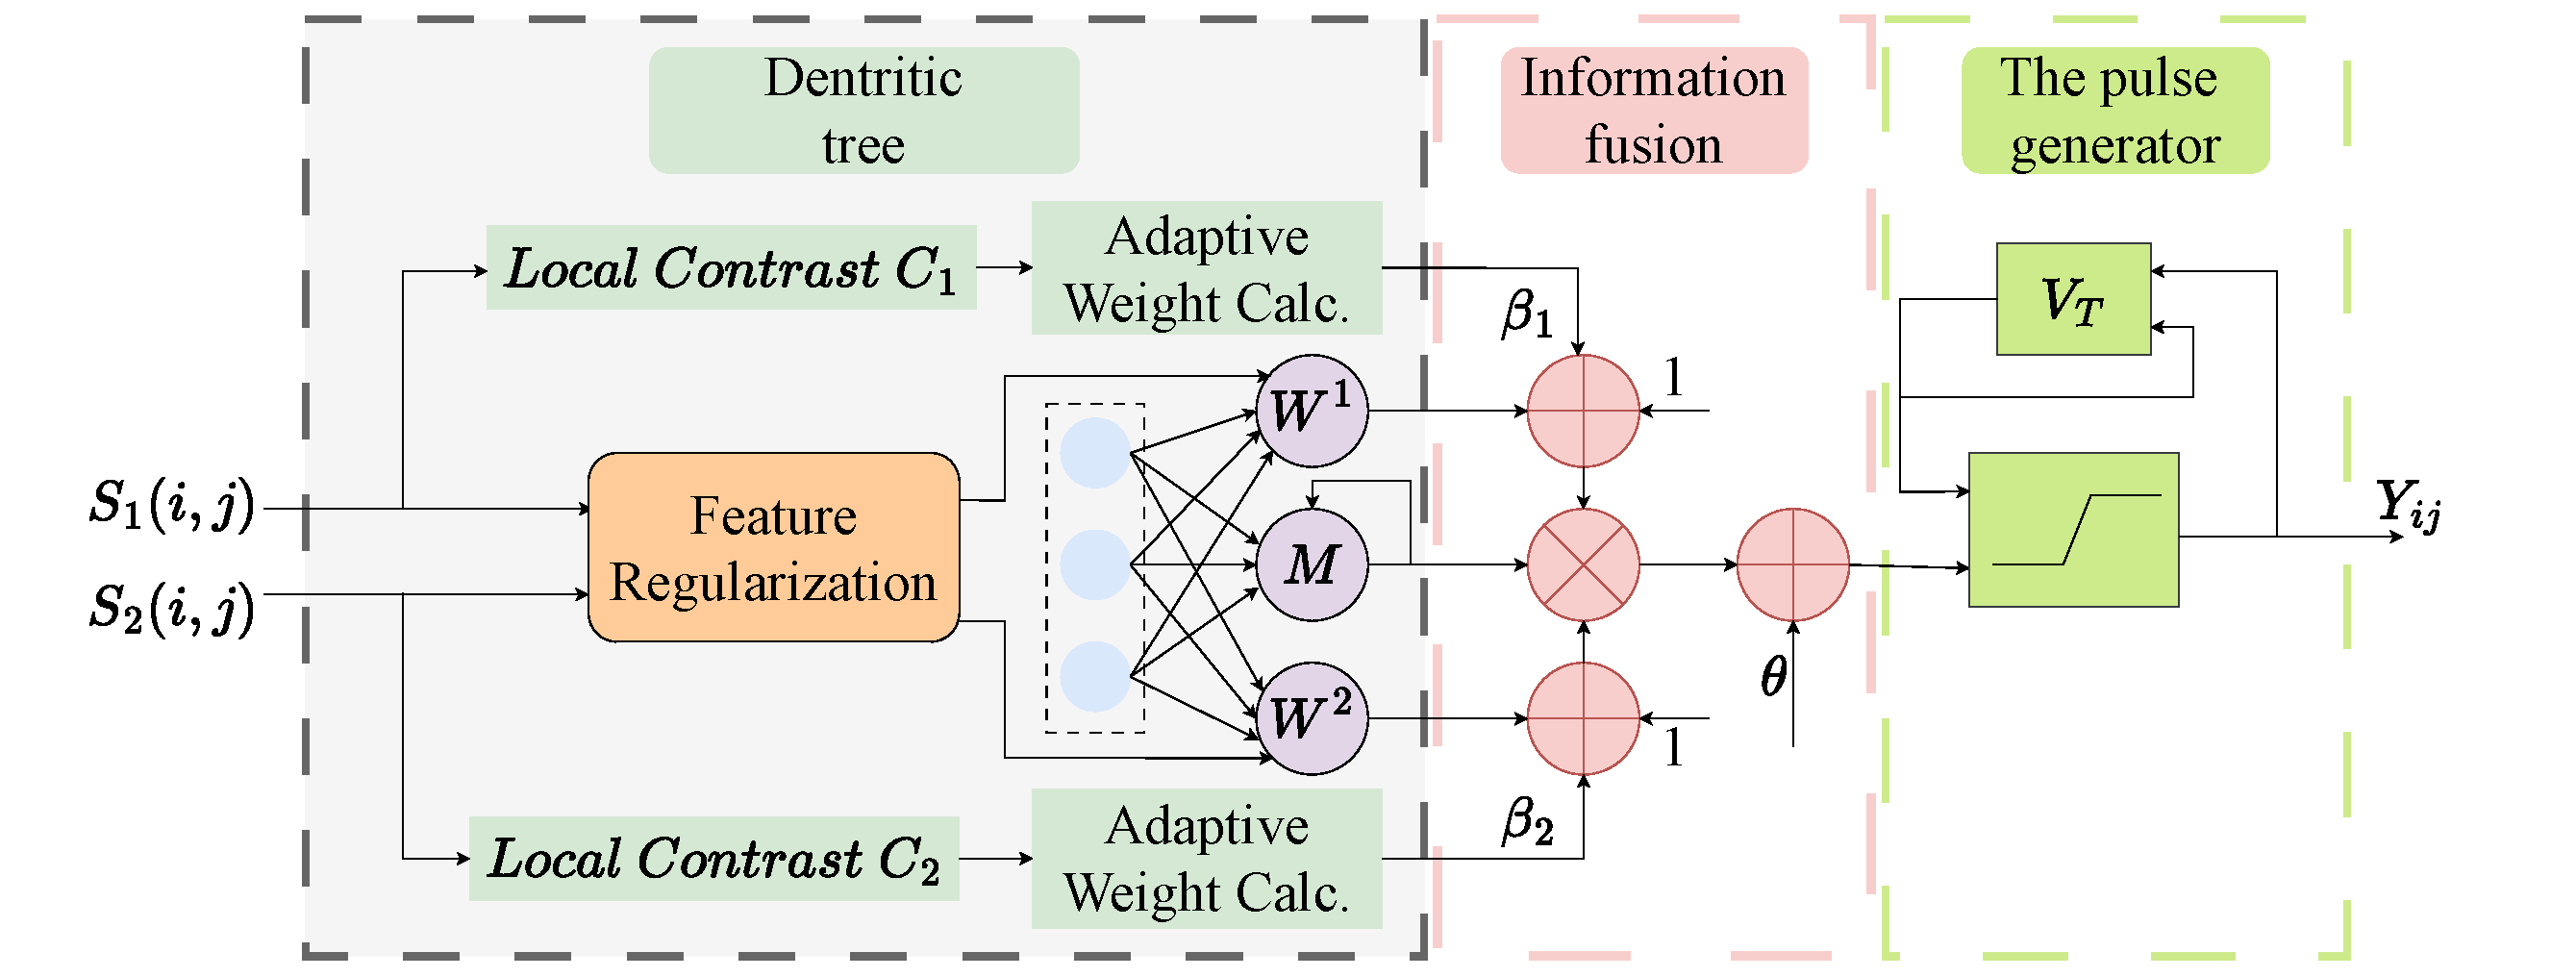
\includegraphics[width=\linewidth]{AW-DPCNN/AW-DPCNN}
	\caption{Architecture of the proposed adaptive weighted dual-channel PCNN (AW-DPCNN) for multi-representation signal fusion. The mechanism comprises contrast-guided adaptive weighting, dual-channel PCNN with representation-specific convolutional kernels, and iterative pulse-coupled dynamics for feature reinforcement.}
	\label{AW-DPCNN}                       
\end{figure}


\begin{figure*}[!t] 
\centering
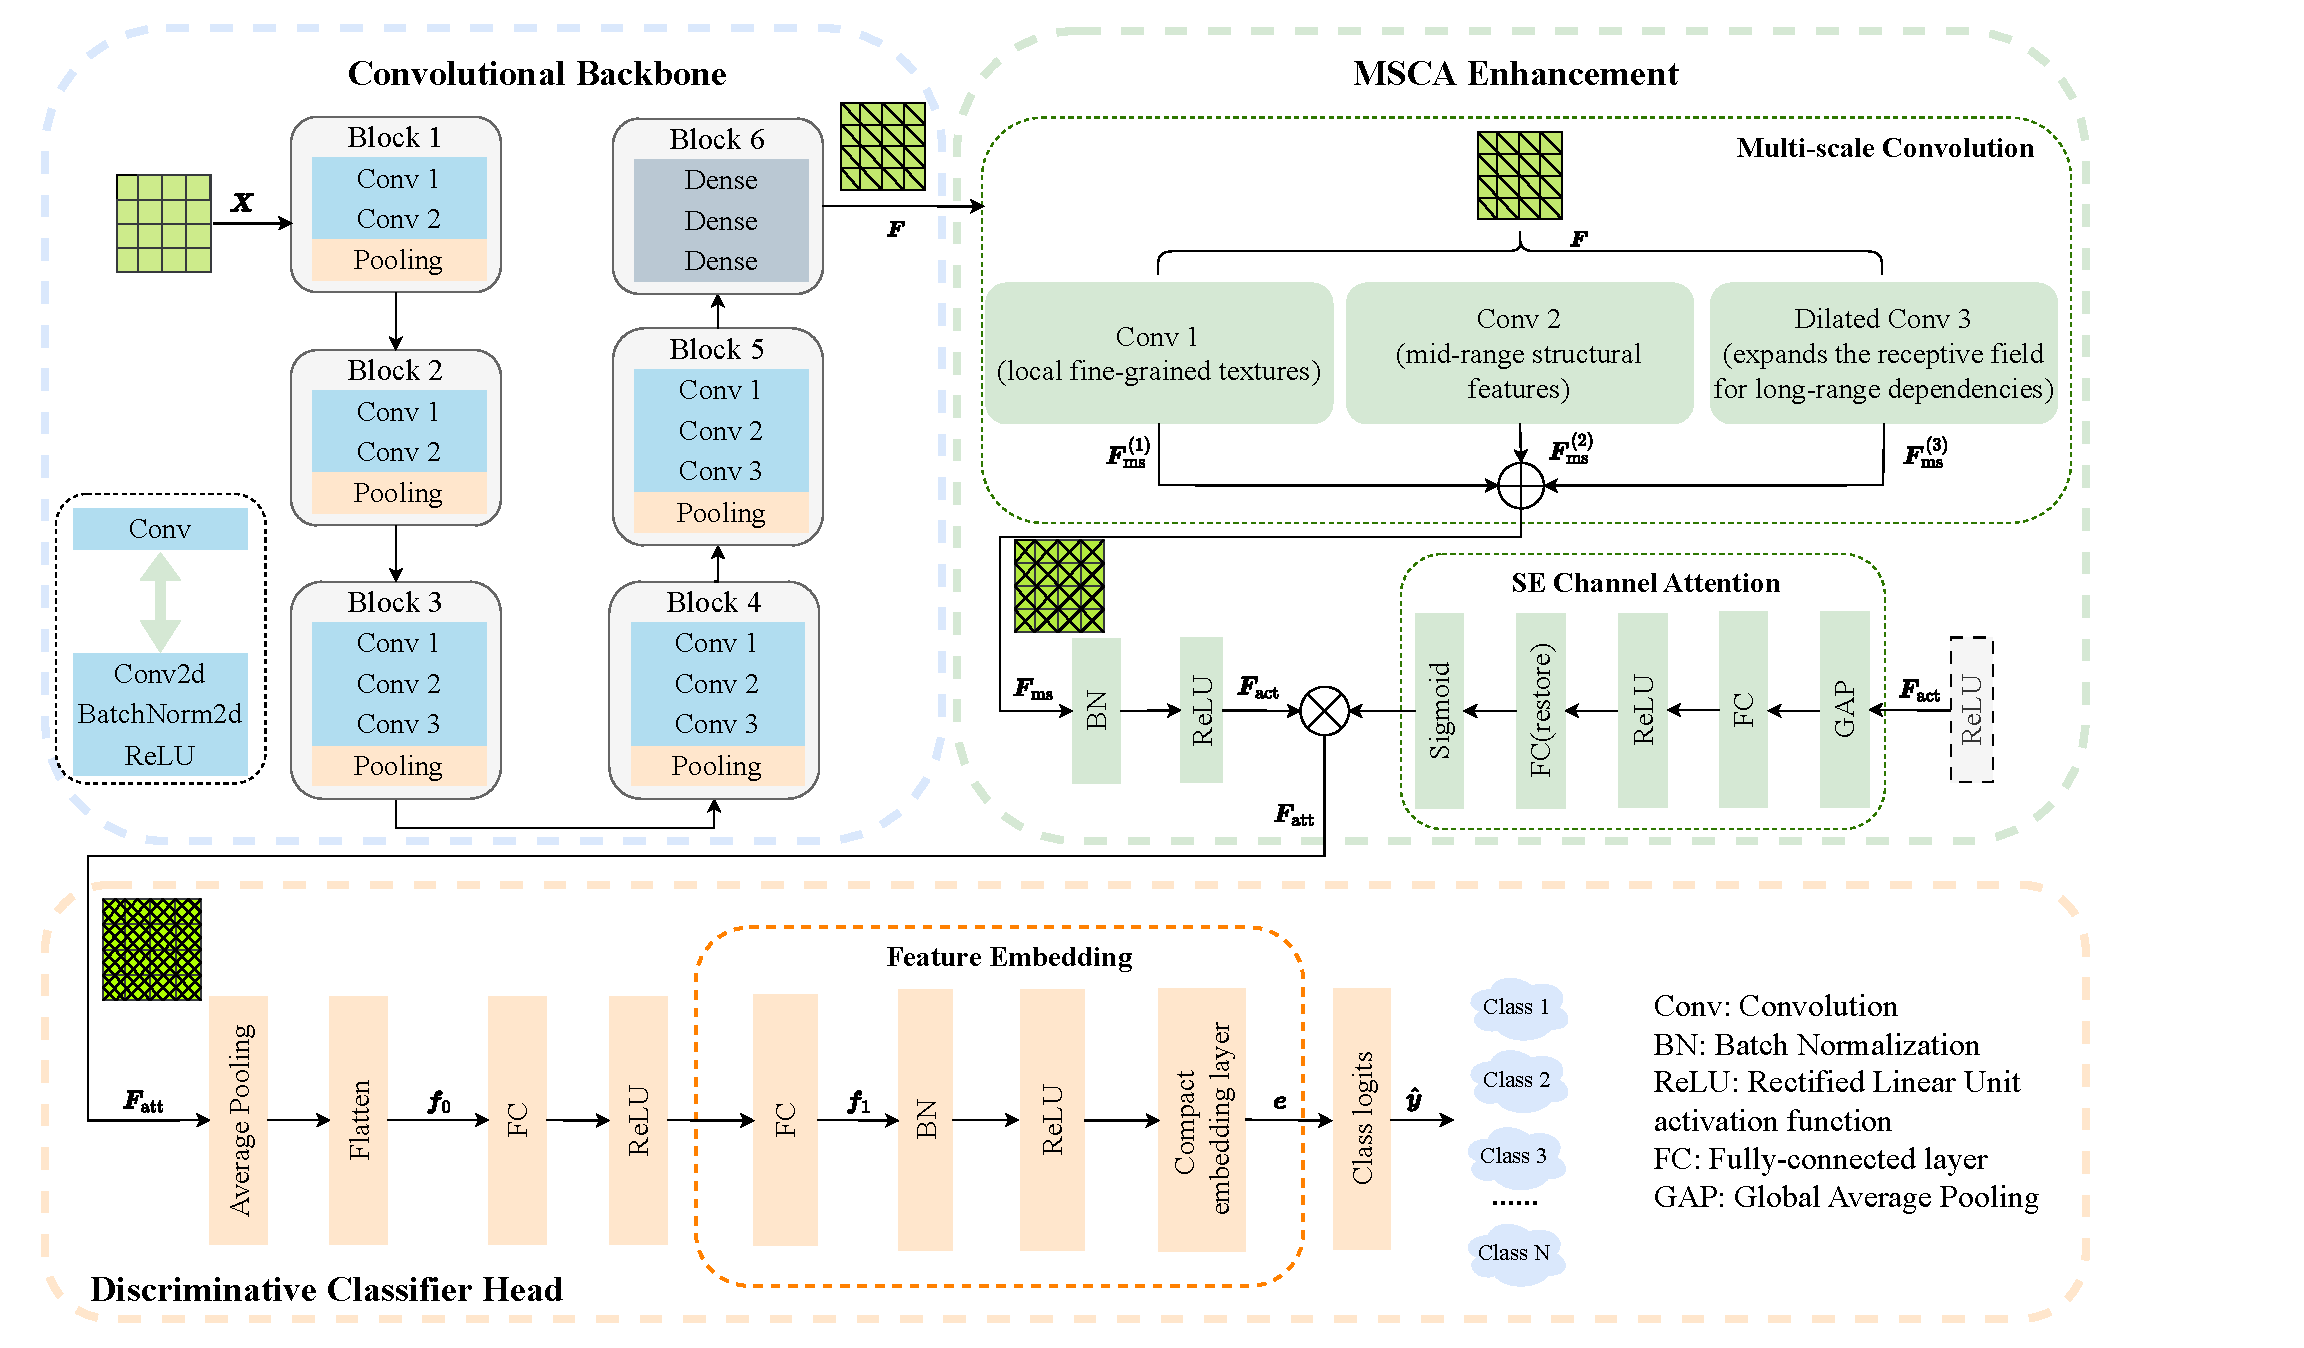
\includegraphics[width=\linewidth]{MSCA-VGG16/MSCA-VGG162.pdf}
\caption{Architecture of the proposed MSCA-VGG16 network. The fused AW-DPCNN image is processed by a VGG16-BN backbone, followed by multi-scale convolution (MS), squeeze-and-excitation channel attention (SE), and a compact embedding head (EH) for fault classification.}
\label{fig:msca_vgg16}
\end{figure*}

\subsection{MSCA-VGG16 for Fused Representation Classification}
\label{sec:msca_vgg16}

The AW-DPCNN fused representations contain heterogeneous features spanning multiple scales and frequency bands. To fully exploit this complementary information, we develop a multi-scale channel attention enhanced network (MSCA-VGG16) built upon three design principles: (i) \emph{multi-scale receptive field alignment} to capture fault patterns at different temporal and spectral granularities; (ii) \emph{dynamic channel recalibration} via squeeze-and-excitation to suppress noise-dominated frequency bands while amplifying fault-sensitive responses; and (iii) \emph{compact discriminative embedding} to project high-dimensional convolutional features into a lower-dimensional space for enhanced intra-class compactness and inter-class separability.

The overall architecture is a modular composition of a convolutional backbone $\mathcal{B}(\cdot)$, a multi-scale channel attention module $\mathcal{M}(\cdot)$, global pooling $\mathcal{P}(\cdot)$, an embedding projection $\mathcal{E}(\cdot)$, and a linear classifier $\mathcal{F}_{cls}(\cdot)$. The forward mapping from input $\boldsymbol{X}$ to predicted class probabilities $\hat{\mathbf{y}}$ is
\begin{equation}
\hat{\mathbf{y}} = \mathcal{F}_{cls}\big(\mathcal{E}\big(\mathcal{P}\big(\mathcal{M}\big(\mathcal{B}(\boldsymbol{X})\big)\big)\big)\big),
\label{eq:cls_pipeline}
\end{equation}
where $\boldsymbol{X} \in \mathbb{R}^{H_0 \times W_0 \times 3}$ denotes the AW-DPCNN fused pseudo-color image of spatial size $H_0 \times W_0$. The overall architecture is illustrated in Fig.~\ref{fig:msca_vgg16}. The following subsections detail each component.

\subsubsection{Convolutional Backbone}

VGG16 with batch normalization (VGG16-BN) is selected as the convolutional backbone. Its purely sequential topology without skip connections, built-in attention, or multi-scale processing provides a clean architectural baseline, ensuring that performance gains can be unambiguously attributed to the multi-scale convolution (MS), channel attention (CA), and embedding head (EH) modules. The backbone maps the fused input image $\boldsymbol{X} \in \mathbb{R}^{H_0 \times W_0 \times 3}$ to a feature map
\begin{equation}
\boldsymbol{F} = \mathcal{B}(\boldsymbol{X}), \quad \boldsymbol{F} \in \mathbb{R}^{H \times W \times C},
\label{eq:feature_map}
\end{equation}
where $H$, $W$, and $C$ denote the spatial height, width, and number of channels, respectively. A comparative validation against alternative backbones is provided in Section~\ref{sec:backbone_comparison}.

\subsubsection{Multi-Scale Convolution Module}

Fault signatures in fused representations span multiple scales, from fine-grained local anomalies to long-range structural correlations. To align the network's receptive field with this multi-scale nature, we introduce a multi-scale convolution module comprising three parallel branches, i.e., a $3\times3$ convolution for local fine-grained textures, a $5\times5$ convolution for mid-range structural features, and a $3\times3$ dilated convolution with rate~2 that expands the receptive field without additional parameters for long-range dependencies. Each branch is formulated as

\begin{equation}
\begin{aligned}
\boldsymbol{F}_{\mathrm{ms}}^{(1)} &= \boldsymbol{\Theta}_{3} * \boldsymbol{F}, \\
\boldsymbol{F}_{\mathrm{ms}}^{(2)} &= \boldsymbol{\Theta}_{5} * \boldsymbol{F}, \\
\boldsymbol{F}_{\mathrm{ms}}^{(3)} &= \boldsymbol{\Theta}_{\mathrm{d}} * \boldsymbol{F},
\end{aligned}
\label{eq:multi_scale_branches}
\end{equation}
where $\boldsymbol{\Theta}_{3}$, $\boldsymbol{\Theta}_{5}$, and $\boldsymbol{\Theta}_{\mathrm{d}}$ denote learnable 2-D convolution kernels, each with $C$ input and $C$ output channels, and with kernel sizes of $3\times3$, $5\times5$, and $3\times3$ (dilation rate $=2$), respectively. Each branch preserves the channel dimensionality $C$ through appropriate padding. The multi-scale features are fused via element-wise summation, which encourages each branch to specialize in complementary scales, i.e.,
\begin{equation}
\boldsymbol{F}_{\mathrm{ms}} = \boldsymbol{F}_{\mathrm{ms}}^{(1)} + \boldsymbol{F}_{\mathrm{ms}}^{(2)} + \boldsymbol{F}_{\mathrm{ms}}^{(3)}.
\label{eq:multi_scale_fusion}
\end{equation}

The aggregated feature map is normalized and activated as follows,
\begin{equation}
\boldsymbol{F}_{\mathrm{act}} = \delta\big(\mathrm{BN}(\boldsymbol{F}_{\mathrm{ms}})\big),
\label{eq:active_feature}
\end{equation}
where $\delta(\cdot) = \max(0, \cdot)$ is the ReLU activation and $\mathrm{BN}(\cdot)$ denotes batch normalization.

\subsubsection{Squeeze-and-Excitation Channel Attention}

Different frequency bands in the fused representation carry unequal diagnostic information. Some channels encode fault-critical spectral components, while others are dominated by background noise or redundant textures. To dynamically recalibrate channel-wise responses, we adopt a squeeze-and-excitation (SE) mechanism after the multi-scale fusion stage.

Let $\boldsymbol{F}_{\mathrm{act}} \in \mathbb{R}^{H \times W \times C}$ be the input to the SE module. The \emph{squeeze} operation aggregates spatial information into a channel descriptor $\boldsymbol{z} \in \mathbb{R}^{C}$ via global average pooling,
\begin{equation}
z_c = \frac{1}{H W} \sum_{i=1}^{H} \sum_{j=1}^{W} \boldsymbol{F}_{\mathrm{act}}(i, j, c), \quad c = 1, \dots, C.
\label{eq:se_squeeze}
\end{equation}

The \emph{excitation} operation models channel-wise dependencies through a bottleneck structure, i.e.,
\begin{equation}
\boldsymbol{s} = \sigma\big(\boldsymbol{U}_2 \, \delta(\boldsymbol{U}_1 \boldsymbol{z})\big),
\label{eq:se_excitation}
\end{equation}
where $\boldsymbol{U}_1 \in \mathbb{R}^{\frac{C}{r} \times C}$ and $\boldsymbol{U}_2 \in \mathbb{R}^{C \times \frac{C}{r}}$ are learnable weight matrices, $r$ is the channel reduction ratio controlling the bottleneck capacity, and $\sigma(\cdot)$ is the sigmoid function. The output $s=[s_1, \dots, s_C]^\mathrm{T}$ represents per-channel attention weights in $[0, 1]$. The refined feature map is obtained by channel-wise rescaling, i.e.,
\begin{equation}
\boldsymbol{F}_{\mathrm{att}}(i, j, c) = s_c \cdot \boldsymbol{F}_{\mathrm{act}}(i, j, c).
\label{eq:attention_feature}
\end{equation}

This mechanism allows the network to emphasize channels containing fault-discriminative information while attenuating noise-dominated channels. The reduction ratio $r$ is specified in the experiment configuration.

\subsubsection{Compact Discriminative Embedding Head}

To promote intra-class compactness and inter-class separation while limiting parameter count, we replace conventional large fully-connected layers with a compact embedding head.

First, the spatially refined feature map $\boldsymbol{F}_{\mathrm{att}}$ is collapsed via global average pooling and flattened, i.e.,
\begin{equation}
\boldsymbol{f}_0 = \mathrm{Flatten}\big(\mathrm{AvgPool}(\boldsymbol{F}_{\mathrm{att}})\big) \in \mathbb{R}^{C}.
\label{eq:flatten_feature}
\end{equation}

Then, a fully-connected projection layer extracts high-level features, i.e.,
\begin{equation}
\boldsymbol{f}_1 = \delta\big(\boldsymbol{W}_{\!fc1}\, \boldsymbol{f}_0\big), \quad \boldsymbol{W}_{\!fc1} \in \mathbb{R}^{D_1 \times C},
\label{eq:fc1_feature}
\end{equation}
and is followed by dropout for regularization, where $D_1$ is the width of the projection layer. A compact embedding layer then projects $\boldsymbol{f}_1$ into a $d$-dimensional discriminative space,
\begin{equation}
\boldsymbol{e} = \delta\big(\mathrm{BN}(\boldsymbol{W}_{\!e}\, \boldsymbol{f}_1)\big), \quad \boldsymbol{e} \in \mathbb{R}^{d},
\label{eq:embedding}
\end{equation}
where $\boldsymbol{W}_{\!e} \in \mathbb{R}^{d \times D_1}$. Batch normalization is applied prior to ReLU to stabilize the feature distribution. Dropout is applied after each activation during training and disabled at inference. Finally, the class logits are obtained via a linear classifier,
\begin{equation}
\hat{\boldsymbol{y}} = \mathrm{softmax}(\boldsymbol{W}_{\!c}\, \boldsymbol{e}), \quad \boldsymbol{W}_{\!c} \in \mathbb{R}^{K \times d},
\label{eq:classifier}
\end{equation}
where $K$ is the number of fault categories. The entire network is optimized by minimizing the cross-entropy loss,
\begin{equation}
\mathcal{L}_{\mathrm{CE}} = -\sum_{k=1}^{K} y_k \log \hat{y}_k,
\label{eq:cross_entropy_loss}
\end{equation}
where $\boldsymbol{y} = [y_1, \dots, y_K]^\mathrm{T}$ is the one-hot ground-truth label.

\subsubsection{Forward Pass Algorithm}

Algorithm~\ref{alg:msca_vgg16} summarizes the complete forward pass of the proposed MSCA-VGG16 network from the fused input image to the predicted class probabilities.

\begin{algorithm}
\caption{Forward Pass of MSCA-VGG16}
\label{alg:msca_vgg16}
\begin{algorithmic}[1]
\Require Fused AW-DPCNN image $\boldsymbol{X} \in \mathbb{R}^{H_0 \times W_0 \times 3}$
\Statex \textbf{Stage 1: Convolutional backbone (VGG16-BN)}
\State Extract backbone feature map $\boldsymbol{F} = \mathcal{B}(\boldsymbol{X})$ \Comment{Eq.~\ref{eq:feature_map}}
\Statex \textbf{Stage 2: Multi-scale convolution (MS)}
\State Compute multi-scale features $\boldsymbol{F}_{\mathrm{ms}}^{(1)}$, $\boldsymbol{F}_{\mathrm{ms}}^{(2)}$, $\boldsymbol{F}_{\mathrm{ms}}^{(3)}$ \Comment{Eq.~\ref{eq:multi_scale_branches}}
\State Fuse branches: $\boldsymbol{F}_{\mathrm{ms}} = \boldsymbol{F}_{\mathrm{ms}}^{(1)} + \boldsymbol{F}_{\mathrm{ms}}^{(2)} + \boldsymbol{F}_{\mathrm{ms}}^{(3)}$ \Comment{Eq.~\ref{eq:multi_scale_fusion}}
\State Normalize and activate: $\boldsymbol{F}_{\mathrm{act}} = \delta(\mathrm{BN}(\boldsymbol{F}_{\mathrm{ms}}))$ \Comment{Eq.~\ref{eq:active_feature}}
\Statex \textbf{Stage 3: Channel attention (SE)}
\State Squeeze spatial context into channel descriptor $\boldsymbol{z}$ \Comment{Eq.~\ref{eq:se_squeeze}}
\State Compute channel attention weights $\boldsymbol{s}$ \Comment{Eq.~\ref{eq:se_excitation}}
\State Recalibrate features: $\boldsymbol{F}_{\mathrm{att}} = \boldsymbol{s} \odot \boldsymbol{F}_{\mathrm{act}}$ \Comment{Eq.~\ref{eq:attention_feature}}
\Statex \textbf{Stage 4: Compact embedding head (EH)}
\State Global average pool and flatten to $\boldsymbol{f}_0$ \Comment{Eq.~\ref{eq:flatten_feature}}
\State Project to $\boldsymbol{f}_1$, then dropout \Comment{Eq.~\ref{eq:fc1_feature}}
\State Compute compact embedding $\boldsymbol{e}$, then dropout \Comment{Eq.~\ref{eq:embedding}}
\Statex \textbf{Stage 5: Classification}
\State Produce class probabilities $\hat{\boldsymbol{y}}$ \Comment{Eq.~\ref{eq:classifier}}
\Ensure Predicted class probabilities $\hat{\boldsymbol{y}} \in \mathbb{R}^{K}$.
\end{algorithmic}
\end{algorithm}



\section{Dataset and Experiments}
\label{section4}
\subsection{Dataset Construction and Preprocessing}
\label{sec:dataset_preprocessing}
The Case Western Reserve University (CWRU) bearing dataset~\footnote{The dataset is available at \url{https://csegroups.case.edu/bearingdatacenter/pages/welcome-page}} is employed as the primary benchmark. The test stand, illustrated in Fig.~\ref{fig:cwru_teststand}, comprises a 2-hp motor, a torque transducer/encoder, a dynamometer, and control electronics. Vibration data were collected using accelerometers placed at the 12 o'clock position on the drive-end (DE) and fan-end (FE) motor housing, digitized at 12~kHz for all experiments and additionally at 48~kHz for DE bearing faults.

Single-point faults of diameters 7, 14, and 21 mils were introduced to the ball, inner race, and outer race of bearings via electro-discharge machining. For the outer race, the fault was located at the 6 o'clock position (orthogonal to the load zone). Together with the healthy baseline, this yields ten categories listed in Table~\ref{tab:operating_conditions}.

For dataset construction, the raw vibration signals are segmented into overlapping windows and converted into pseudo-color fused images through the AW-DPCNN pipeline. Three dataset variants are constructed to support comprehensive evaluation as follows.
\begin{enumerate}
\item \textbf{CWRU 12k DE (primary benchmark):} 12~kHz drive-end signals, window length 2048 samples, hop length 1024 samples, $n_{\text{fft}}=1024$, yielding $\Delta f=11.7$~Hz/bin.
\item \textbf{CWRU 12k FE (cross-sensor generalization):} 12~kHz fan-end signals with identical time--frequency parameters, enabling evaluation of sensor-position transferability.
\item \textbf{CWRU 48k DE (cross-sampling-rate generalization):} 48~kHz drive-end signals, window length 8192 samples, hop length 4096 samples, $n_{\text{fft}}=4096$, maintaining identical $\Delta f=11.7$~Hz/bin with $f_{\max}$ extended to 24~kHz.
\end{enumerate}

The window and hop lengths are scaled proportionally with the sampling rate to ensure that every fused image represents the same physical duration of vibration signal, eliminating temporal-scale confounds from cross-dataset comparisons. File-level stratified splitting is applied with a 60\%/20\%/20\% (train/validation/test) ratio, using a fixed random seed (42) for reproducibility. All windows from a given source recording are assigned exclusively to a single split to prevent data leakage. The detailed dataset composition, including sample counts per class and per split, is provided in Table~\ref{tab:datasets_comprehensive}.

For the primary benchmark (12k DE), the normal class contains substantially more windows than the fault classes (see Table~\ref{tab:datasets_comprehensive}) because the normal baseline recordings are approximately four times longer. This inherent class imbalance is addressed through class-weighted cross-entropy loss and macro-averaged evaluation metrics. All datasets use the linear STFT spectrogram as the time--frequency representation and GADF as the temporal encoding, with the optimal combination validated through systematic representation comparison experiments in Section~\ref{sec:rep_compare}.


\begin{table}[!t]
	\caption{Operating Conditions and Corresponding Labels of the CWRU Bearing Dataset\label{tab:operating_conditions}}
	\centering
	\begin{tabular}{ll}
		\toprule
		Label & Description \\
		\midrule
		Normal & Healthy Baseline \\
		BF007 & Ball Fault (0.007'') \\ 
		BF014 & Ball Fault (0.014'') \\
		BF021 & Ball Fault (0.021'') \\
		IF007 & Inner Race Fault (0.007'') \\
		IF014 & Inner Race Fault (0.014'') \\
		IF021 & Inner Race Fault (0.021'') \\
		OF007 & Outer Race Fault @6 (0.007'') \\
		OF014 & Outer Race Fault @6 (0.014'') \\
		OF021 & Outer Race Fault @6 (0.021'') \\
		
		\bottomrule
	\end{tabular}
\end{table}


\begin{table}[!t]
\caption{Class-Wise Sample Distribution of Three CWRU Bearing Datasets\label{tab:datasets_comprehensive}}
\centering
\renewcommand{\arraystretch}{1.0}
\setlength{\tabcolsep}{5pt}
\begin{tabular}{lcccc}
\toprule
\textbf{Dataset} & \textbf{Class} & \textbf{Train} & \textbf{Val} & \textbf{Test} \\
\midrule
\multirow{11}{*}{\textbf{CWRU 12k DE}} 
& BF007  & 234 & 117 & 118 \\
& BF014  & 236 & 117 & 118 \\
& BF021  & 235 & 118 & 118 \\
& IF007  & 236 & 117 & 119 \\
& IF014  & 234 & 117 & 117 \\
& IF021  & 235 & 117 & 118 \\
& OF007  & 236 & 118 & 117 \\
& OF014  & 234 & 118 & 118 \\
& OF021  & 236 & 118 & 118 \\
& Normal & 708 & 473 & 471 \\
& \textbf{Total} & \textbf{2824} & \textbf{1530} & \textbf{1532} \\
\midrule
\multirow{11}{*}{\textbf{CWRU 12k FE}} 
& BF007  & 233 & 117 & 117 \\
& BF014  & 235 & 118 & 117 \\
& BF021  & 233 & 117 & 117 \\
& IF007  & 234 & 117 & 117 \\
& IF014  & 234 & 117 & 117 \\
& IF021  & 234 & 117 & 117 \\
& OF007  & 235 & 117 & 117 \\
& OF014  & 69  & 22  & 22  \\
& OF021  & 69  & 22  & 22  \\
& Normal & 708 & 473 & 471 \\
& \textbf{Total} & \textbf{2484} & \textbf{1337} & \textbf{1334} \\
\midrule
\multirow{11}{*}{\textbf{CWRU 48k DE}} 
& BF007  & 234 & 118 & 58  \\
& BF014  & 234 & 59  & 117 \\
& BF021  & 234 & 117 & 58  \\
& IF007  & 234 & 58  & 117 \\
& IF014  & 236 & 117 & 14  \\
& IF021  & 235 & 118 & 58  \\
& OF007  & 235 & 58  & 117 \\
& OF014  & 175 & 117 & 118 \\
& OF021  & 236 & 59  & 118 \\
& Normal & 175 & 117 & 117 \\
& \textbf{Total} & \textbf{2228} & \textbf{938}  & \textbf{892}  \\
\bottomrule
\end{tabular}
\end{table}


\begin{figure*}[!t]
	\centering
	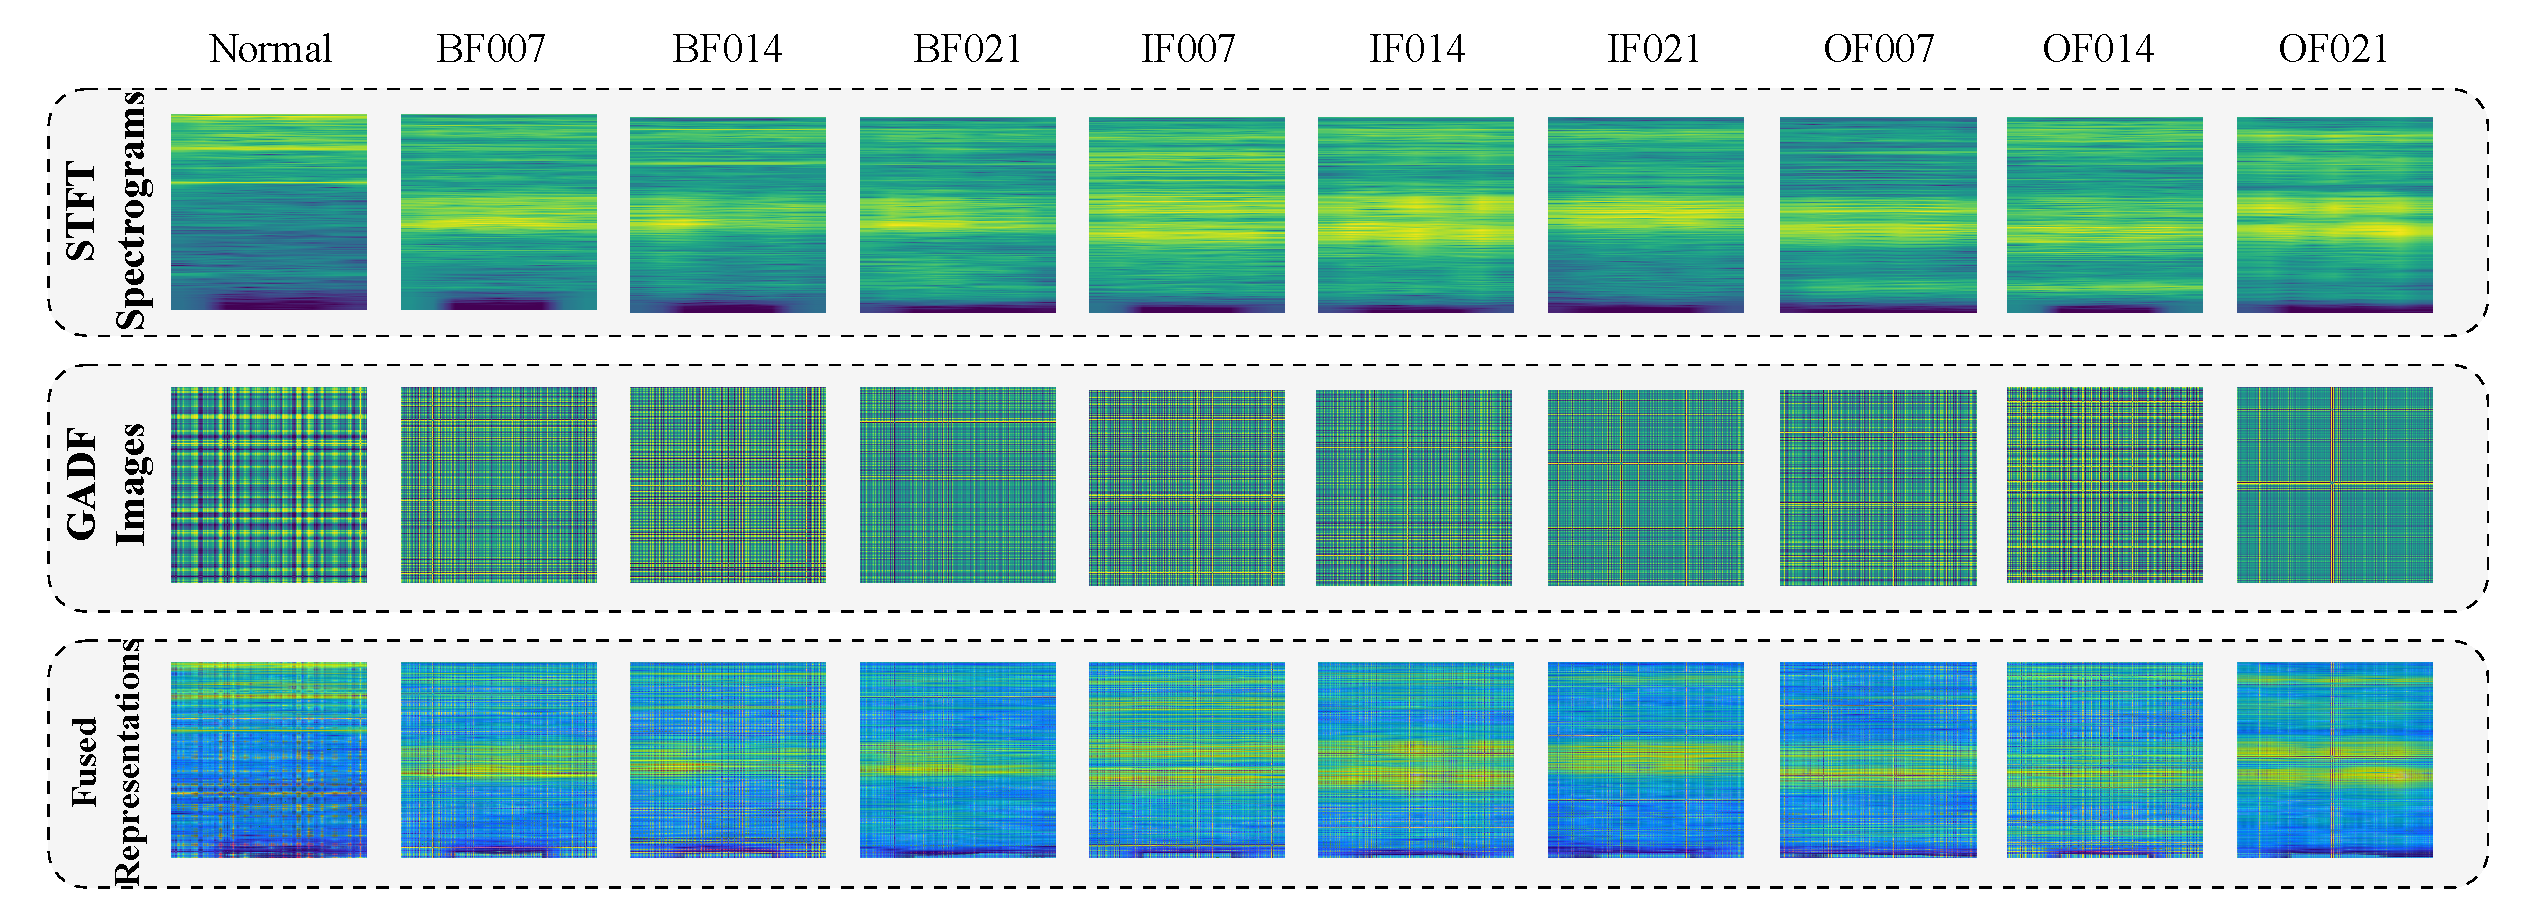
\includegraphics[width=\textwidth]{Fused images/Fused images2}
	\caption{STFT spectrograms (top), GADF images (middle), and AW-DPCNN fused representations (bottom) for ten bearing conditions.}
	\label{fig:fused_images}
\end{figure*}
Fig.~\ref{fig:fused_images} illustrates the representations before and after adaptive fusion. The fused outputs exhibit enhanced structural clarity, i.e., background noise is suppressed while fault-discriminative features are preserved, demonstrating that AW-DPCNN effectively integrates complementary time--frequency and temporal-domain information.
\subsection{Implementation Details and Evaluation Metrics}

\begin{figure}[!t]
	\centering
	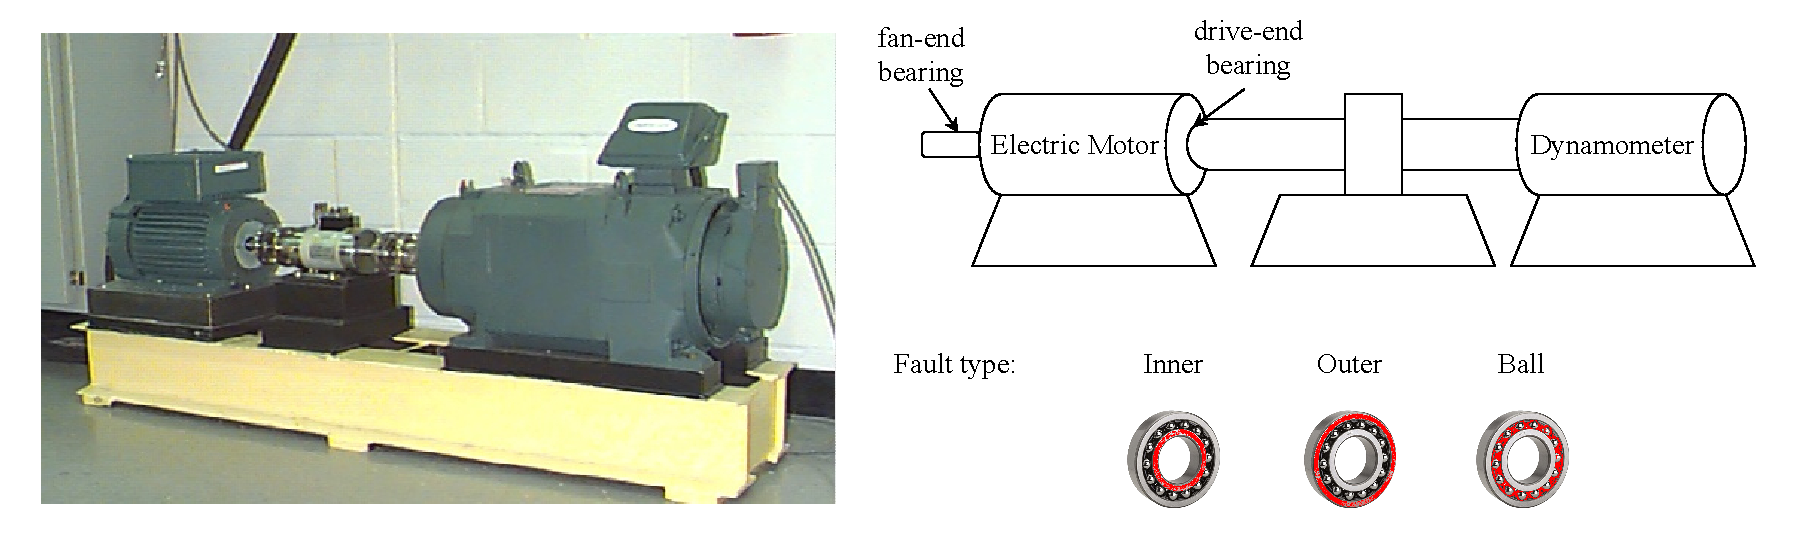
\includegraphics[width=\linewidth]{equipment/cwru1}
	\caption{CWRU bearing test stand. Vibration signals were collected from accelerometers at the drive-end and fan-end positions under four operating loads (0--3 hp).}
	\label{fig:cwru_teststand}
\end{figure}

The raw vibration signals are converted into STFT spectrograms and GADF images, fused via AW-DPCNN, and resized to $224 \times 224$ pseudo-color RGB images as input to the MSCA-VGG16 network.

To mitigate class imbalance, a class-weighted cross-entropy loss is adopted. The weight for class $k$ is computed as
\begin{equation}
w_k = \frac{N_{\mathrm{total}}}{K \cdot N_k},
\label{eq:class_weight}
\end{equation}
where $N_{\mathrm{total}}$ denotes the total number of training samples, $K$ is the number of fault categories, and $N_k$ is the number of training samples belonging to class $k$. The weighted cross-entropy loss is then formulated as
\begin{equation}
\mathcal{L}_{\mathrm{wCE}} = -\frac{1}{B} \sum_{i=1}^{B} w_{y_i} \sum_{k=1}^{K} \boldsymbol{y}_{i,k} \log \hat{\boldsymbol{y}}_{i,k},
\label{eq:weighted_ce}
\end{equation}
where $w_{y_i}$ is the class weight of the ground-truth label, $\boldsymbol{y}_{i,k}$ is the $k$-th entry of the one-hot encoded label vector, and $\hat{\boldsymbol{y}}_{i,k}$ is the predicted probability for class $k$. This weighting strategy ensures that minority classes receive proportionally larger loss contributions, preventing the model from being biased toward majority classes.

All models are optimized using AdamW with an initial learning rate $\eta=1\times10^{-4}$ and weight decay $\lambda=1\times10^{-3}$. A ReduceLROnPlateau scheduler reduces the learning rate by a factor of $0.5$ when the validation F1-score does not improve for 5 consecutive epochs, down to a minimum of $\eta_{\min}=1\times10^{-6}$. Training uses a batch size of 32 for up to 30 epochs. Data augmentation consists of random horizontal flipping (probability 0.5) and random rotation within $\pm10^\circ$. Input images are normalized using ImageNet statistics, which aligns with the pretrained VGG16-BN backbone. Early stopping is triggered if the validation macro-averaged F1-score does not improve for 15 consecutive epochs, and the model checkpoint with the highest validation F1-score is retained for final evaluation on the held-out test set.

To ensure statistical reliability and to account for performance variance due to random initialization, all key experiments are repeated over three independent trials with different random seeds (42, 123, 456). The aggregated results are reported as mean $\pm$ standard deviation across the three trials.

The experiments in this study were conducted on a system equipped with an Intel i9-14900K CPU and an NVIDIA RTX 5090 GPU. The software environment was based on PyTorch 2.11 and CUDA 13.0. Classification performance is evaluated using accuracy, precision, recall, macro-averaged F1-score, balanced accuracy (B-Acc), G-mean, Cohen's kappa, and the area under the receiver operating characteristic curve (ROC-AUC). For multi-class ROC-AUC, the One-vs-Rest (OvR) macro-averaged AUC is reported.






\begin{figure}[!t]
	\centering
	\begin{subfigure}{0.48\columnwidth}
		\centering
		\includegraphics[width=\columnwidth]{../experiments/experiment_result/rep_compare/stft_gadf/rep_compare_stft_gadf/trial_seed42/figures/confusion_matrix.png}
		\caption{STFT + GADF}
	\end{subfigure}
	\hfill
	\begin{subfigure}{0.48\columnwidth}
		\centering
		\includegraphics[width=\columnwidth]{../experiments/experiment_result/rep_compare/mel_gadf/rep_compare_mel_gadf/trial_seed42/figures/confusion_matrix.png}
		\caption{Mel + GADF}
	\end{subfigure}
	\caption{Confusion matrices of the best-performing (STFT + GADF) and worst-performing (Mel + GADF) representation combinations. STFT + GADF exhibits substantially reduced inter-class confusion, particularly among fault severity levels.}
	\label{fig:rep_compare_cm}
\end{figure}

% Auto-generated by scripts/analyze_results.py
% Date: 2026-06-30 17:37:58
% These tables can be \input{} directly into tim.tex
% ── Representation Comparison Table ──
\begin{table*}
    \centering
    \caption{Representation Comparison Across Time--Frequency and Temporal Encoding Methods. All combinations are fused via AW-DPCNN and classified by standard VGG16 network trained from scratch. Best values per metric are bolded.}
    \label{tab:rep_compare}
    \renewcommand{\arraystretch}{1.15}
    \small
    \begin{tabular}{llcccc}
        \toprule
        \textbf{TF Method} & \textbf{Temporal} & \textbf{Acc (\%)} & \textbf{F1 (\%)} & \textbf{G-mean (\%)} & \textbf{AUC (\%)} \\
        \midrule
        \multirow{4}{*}{Mel} & GADF & $89.18 \pm 1.87$ & $83.94 \pm 3.64$ & $77.27 \pm 6.99$ & $99.46 \pm 0.23$ \\
         & GASF & $93.53 \pm 2.22$ & $90.52 \pm 4.02$ & $86.27 \pm 8.92$ & $99.44 \pm 0.43$ \\
         & MTF & $94.08 \pm 1.08$ & $90.94 \pm 2.08$ & $86.27 \pm 4.76$ & $99.62 \pm 0.17$ \\
         & RP & $94.56 \pm 3.61$ & $92.55 \pm 4.96$ & $90.93 \pm 6.56$ & $99.57 \pm 0.36$ \\
        \cmidrule(lr){2-6}
        \multirow{4}{*}{STFT} & GADF & $\mathbf{96.30 \pm 0.49}$ & $\mathbf{95.02 \pm 0.40}$ & $\mathbf{94.22 \pm 0.49}$ & $\mathbf{99.97 \pm 0.03}$ \\
         & GASF & $91.23 \pm 0.65$ & $85.86 \pm 0.79$ & $69.32 \pm 8.26$ & $99.38 \pm 0.27$ \\
         & MTF & $90.16 \pm 7.46$ & $86.48 \pm 9.50$ & $78.92 \pm 17.99$ & $98.16 \pm 2.81$ \\
         & RP & $90.12 \pm 0.95$ & $84.28 \pm 0.95$ & $39.34 \pm 26.45$ & $99.35 \pm 0.04$ \\
        \cmidrule(lr){2-6}
        \multirow{4}{*}{CWT} & GADF & $89.70 \pm 1.53$ & $84.32 \pm 2.55$ & $76.01 \pm 6.93$ & $99.33 \pm 0.16$ \\
         & GASF & $89.81 \pm 1.30$ & $85.75 \pm 2.14$ & $80.87 \pm 3.91$ & $99.14 \pm 0.17$ \\
         & MTF & $90.01 \pm 2.72$ & $85.24 \pm 4.42$ & $77.00 \pm 9.29$ & $99.16 \pm 0.50$ \\
         & RP & $90.88 \pm 0.04$ & $87.43 \pm 0.39$ & $83.95 \pm 1.41$ & $98.99 \pm 0.13$ \\
        \bottomrule
    \end{tabular}
\end{table*}

\subsection{Representation Comparison}
\label{sec:rep_compare}



To empirically justify the choice of STFT and GADF as the input representations, twelve combinations of three time--frequency representations and four temporal encoding methods are systematically compared. All representations are fused through the identical AW-DPCNN pipeline ($\gamma=10$, $N=20$) and classified using a standard VGG16 network trained from scratch, thereby isolating the effect of the input representation on diagnostic performance. All other training settings follow Section~\ref{sec:dataset_preprocessing} and are kept identical across runs.



Table~\ref{tab:rep_compare} reports the test set performance of all twelve combinations. In addition to the superior accuracy and F1-score, the STFT+GADF pair achieves the highest AUC (99.97\%), converges to the best validation F1-score within approximately 9 epochs, notably fewer than competing combinations, and produces the most compact and well-separated confusion patterns (Fig.~\ref{fig:rep_compare_cm}). Several important observations emerge as follows.

\textbf{1) Time--frequency representation comparison.} Among the three time--frequency methods, the STFT spectrogram consistently achieves the highest accuracy when paired with GADF (96.30\%), substantially outperforming the best Mel-based combination (Mel and RP, 94.56\%) and the best CWT-based combination (CWT and RP, 90.88\%). The uniform frequency resolution of the linear STFT spectrogram preserves fine-grained high-frequency fault signatures that are essential for distinguishing between different bearing fault severities, whereas the Mel-scale's nonlinear frequency compression and the CWT's variable resolution may obscure these discriminative spectral details.

\textbf{2) Temporal encoding comparison.} Among the four temporal encoding methods, GADF achieves the best performance when paired with STFT (96.30\%), significantly outperforming GASF (91.23\%), MTF (90.16\%), and RP (90.12\%). The GADF's angular difference encoding captures more discriminative temporal transition patterns than the summation-based GASF, and the structured correlation matrix provides richer information than the quantized transition probabilities of MTF or the binary recurrence patterns of RP. Notably, GADF paired with STFT achieves a G-mean of 94.22\%, far exceeding the next best combination (Mel and RP, 90.93\%), confirming that the STFT and GADF pair provides the most balanced class-wise discrimination.

\textbf{3) Optimal combination.} The STFT spectrogram paired with GADF achieves the best overall performance across all metrics, with 96.30\% accuracy, 95.02\% F1-score, and 94.22\% G-mean. This result empirically validates the choice of STFT and GADF as the input representation pair for the proposed AW-DPCNN framework. The STFT spectrogram provides uniform-resolution time--frequency energy distributions, while the GADF encodes complementary temporal correlation structures through angular differences, forming a jointly discriminative basis for bearing fault diagnosis. The representation comparison also reveals that some non-optimal pairs (e.g., Mel and RP at 94.56\%) can achieve competitive accuracy, suggesting that the AW-DPCNN fusion mechanism is sufficiently robust to extract discriminative features from suboptimal input representations, though the optimal STFT and GADF pair provides the best performance with the lowest variance.



These results collectively demonstrate that the STFT and GADF combination provides the most effective input representation for the AW-DPCNN fusion framework, offering consistent advantages over alternative time--frequency and temporal encoding methods. The empirical evidence supports the representation design adopted in this work and further validates the robustness of the proposed diagnostic pipeline.


	\begin{figure*}[!t]
		\centering
		\begin{subfigure}{0.32\linewidth}
			\centering
			\includegraphics[width=\linewidth]
			{../experiments/experiment_result/exp1/convnext_tiny/12k_de/exp1_convnext_tiny/trial_seed42/figures/confusion_matrix.png}
			\caption{ConvNeXt-Tiny}
		\end{subfigure}
		\hfill
		\begin{subfigure}{0.32\linewidth}
			\centering
			\includegraphics[width=\linewidth]
			{../experiments/experiment_result/exp1/efficientnet_b0/12k_de/exp1_efficientnet_b0/trial_seed456/figures/confusion_matrix.png}
			\caption{EfficientNet-B0}
		\end{subfigure}
		\hfill
		\begin{subfigure}{0.32\linewidth}
			\centering
			\includegraphics[width=\linewidth]
			{../experiments/experiment_result/exp1/vit/12k_de/exp1_vit/trial_seed42/figures/confusion_matrix.png}
			\caption{ViT}
		\end{subfigure}

		\vspace{2mm}

		\begin{subfigure}{0.32\linewidth}
			\centering
			\includegraphics[width=\linewidth]{../experiments/experiment_result/exp1/mobilenetv3_small/12k_de/exp1_mobilenetv3_small/trial_seed42/figures/confusion_matrix.png}
			\caption{MobileNetV3-Small}
		\end{subfigure}
		\hfill
		\begin{subfigure}{0.32\linewidth}
			\centering
			\includegraphics[width=\linewidth]{../experiments/experiment_result/exp1/vgg16/12k_fe/exp1_vgg16/trial_seed123/figures/confusion_matrix.png}
			\caption{VGG16}
		\end{subfigure}
		\hfill
		\begin{subfigure}{0.32\linewidth}
			\centering
			\includegraphics[width=\linewidth]{../experiments/experiment_result/exp1/MSCA_VGG16/12k_de/exp1_MSCA_VGG16/trial_seed42/figures/confusion_matrix.png}
			\caption{MSCA-VGG16 (Ours)}
		\end{subfigure}
		\caption{Confusion matrices of different network backbones trained using the AW-DPCNN fusion representations on the CWRU 12k DE dataset. The proposed MSCA-VGG16 achieves the most accurate classification with significantly reduced inter-class confusion.}
		\label{fig:confusion_matrix}
	\end{figure*}

% Auto-generated by scripts/analyze_results.py
% Date: 2026-06-30 17:37:58
% These tables can be \input{} directly into tim.tex
% ── Backbone Comparison Table ──
\begin{table*}
    \caption{Performance Comparison with Different Backbone Networks\label{tab:network_comparison}}
    \centering
    \renewcommand{\arraystretch}{1.15}
    \begin{tabular}{lcccccc}
        \toprule
        \textbf{Network} & \textbf{Acc (\%)} & \textbf{Recall (\%)} & \textbf{F1 (\%)} & \textbf{G-mean (\%)} & \textbf{B-Acc (\%)} & \textbf{Kappa (\%)} \\
        \midrule
        % \textbf{MSCA-VGG16 (Ours)} & $\mathbf{99.85 \pm 0.10}$ & $\mathbf{99.80 \pm 0.13}$ & $\mathbf{99.80 \pm 0.13}$ & $\mathbf{99.80 \pm 0.13}$ & $\mathbf{99.80 \pm 0.13}$ & $\mathbf{99.82 \pm 0.12}$ \\
        % \textbf{MSCA-VGG16 (Ours)} & $\mathbf{99.85 \pm 0.10}$ & $\mathbf{99.80 \pm 0.13}$ & $\mathbf{99.80 \pm 0.13}$ & $\mathbf{99.80 \pm 0.13}$ & $\mathbf{99.80 \pm 0.13}$ & $\mathbf{99.82 \pm 0.12}$ \\
        \textbf{MSCA-VGG16 (Ours)} & $\mathbf{99.85 \pm 0.10}$ & $\mathbf{99.84 \pm 0.22}$ & $\mathbf{99.46 \pm 0.43}$ & $\mathbf{99.82 \pm 0.15}$ & $\mathbf{99.86 \pm 0.13}$ & $\mathbf{99.82 \pm 0.12}$ \\
        VGG16 (Peng et al.\cite{9440949}) & $99.19 \pm 0.89$ & $98.95 \pm 1.16$ & $98.95 \pm 1.16$ & $98.91 \pm 1.22$ & $98.95 \pm 1.16$ & $99.06 \pm 1.05$ \\
        EfficientNet-B0 (Cheng et al.\cite{11028059})& $95.74 \pm 2.07$ & $94.47 \pm 2.68$ & $94.14 \pm 3.05$ & $93.08 \pm 4.09$ & $94.47 \pm 2.68$ & $95.00 \pm 2.43$ \\
        ViT (Liu et al.\cite{10663388}) & $82.35 \pm 0.89$ & $77.20 \pm 1.06$ & $74.71 \pm 2.19$ & $64.72 \pm 7.53$ & $77.20 \pm 1.06$ & $79.30 \pm 1.04$ \\
        MobileNetV3-Small (Zhang et al.\cite{ZHANG2026106301})& $93.69 \pm 1.64$ & $91.81 \pm 2.13$ & $91.03 \pm 2.69$ & $87.82 \pm 5.30$ & $91.81 \pm 2.13$ & $92.60 \pm 1.92$ \\
        ResNet18 (Duan et al.\cite{DUAN2026122469})& $ 98.39\pm 1.32$ & $97.91 \pm 1.71$ & $97.85 \pm1.81 $ & $ 97.66 \pm 2.10$ & $ 97.91\pm 1.71$ & $ 98.11\pm 1.55$ \\
        ConvNeXt-Tiny (Tu et al.\cite{10929672})& $92.93 \pm 2.12$ & $90.82 \pm 2.76$ & $90.63 \pm 2.50$ & $88.99 \pm 3.11$ & $90.82 \pm 2.76$ & $91.70 \pm 2.49$ \\
        \midrule
        VGG16 (STFT only\cite{9440949}) & $93.37\pm 1.32$ & $92.71 \pm1.45 $ & $91.49 \pm 2.25$ & $86.89\pm 5.47$ & $ 92.71\pm1.45 $ & $92.58\pm 1.48$ \\
        VGG16 (GADF only\cite{9440949}) & $60.99\pm 1.50$ & $ 62.71\pm 2.51$ & $ 56.90\pm 2.13$ & $ 12.93\pm 1.42$ & $ 62.71\pm 2.51$ & $ 56.75\pm 1.37$ \\
        \bottomrule
    \end{tabular}
\end{table*}

\subsection{Backbone Comparison}
\label{sec:backbone_comparison}

To evaluate the effectiveness of the proposed classification network, seven representative deep learning backbones are compared under identical settings, with results reported as mean $\pm$ standard deviation over three independent trials in Table~\ref{tab:network_comparison}.

MSCA-VGG16 achieves the highest overall performance, i.e., 99.85\% accuracy, 99.46\% F1-score, and 99.82\% G-mean, outperforming the second-best VGG16 baseline by 0.66\% (99.19\%) and the widely-used ResNet18 by 1.46\% (98.39\%). This margin confirms that the multi-scale convolution, channel attention, and compact embedding modules each contribute meaningful gains beyond the VGG16 backbone alone. Among the remaining architectures, EfficientNet-B0 (95.74\%), MobileNetV3-Small (93.69\%), ConvNeXt-Tiny (92.93\%), and ViT (82.35\%) all underperform substantially, with ViT's poor result confirming that transformer-based architectures are ill-suited for the small-scale CWRU dataset where convolutional inductive biases provide stronger priors.


\begin{figure*}[!t]
	\centering
	\begin{subfigure}{0.32\textwidth}
		\centering
		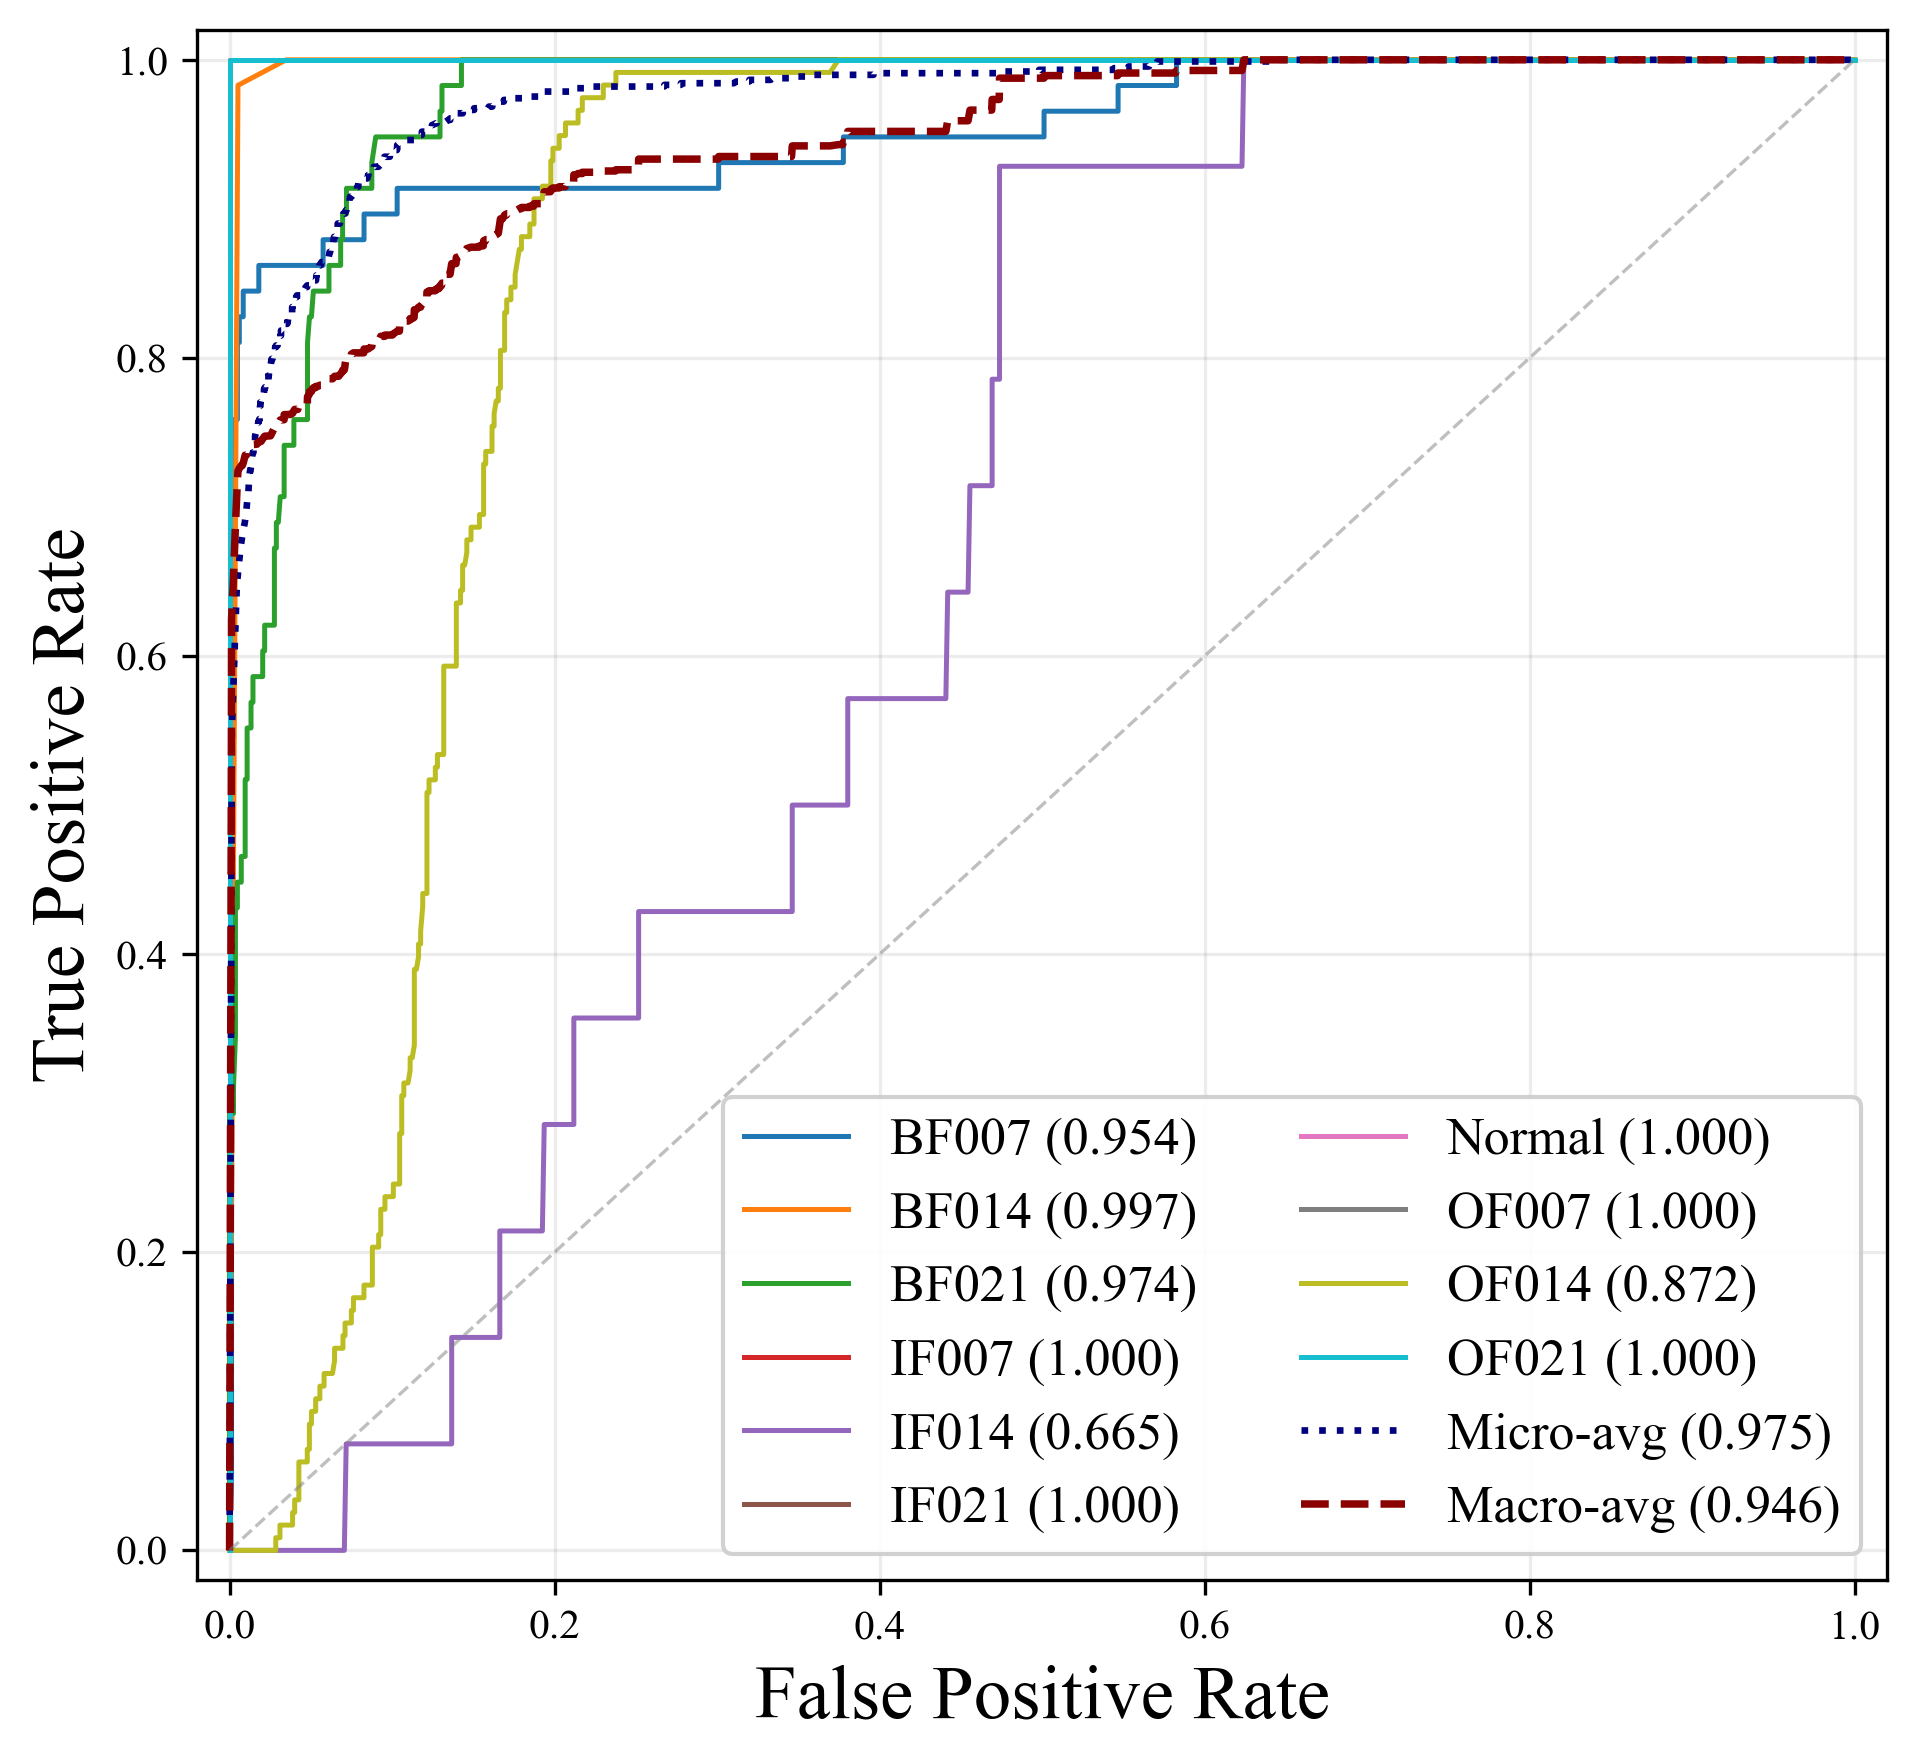
\includegraphics[width=\linewidth]{figures/roc/convnext-tiny_roc.png}
		\caption{ConvNeXt-Tiny}
	\end{subfigure}
	\hfill
	\begin{subfigure}{0.32\textwidth}
		\centering
		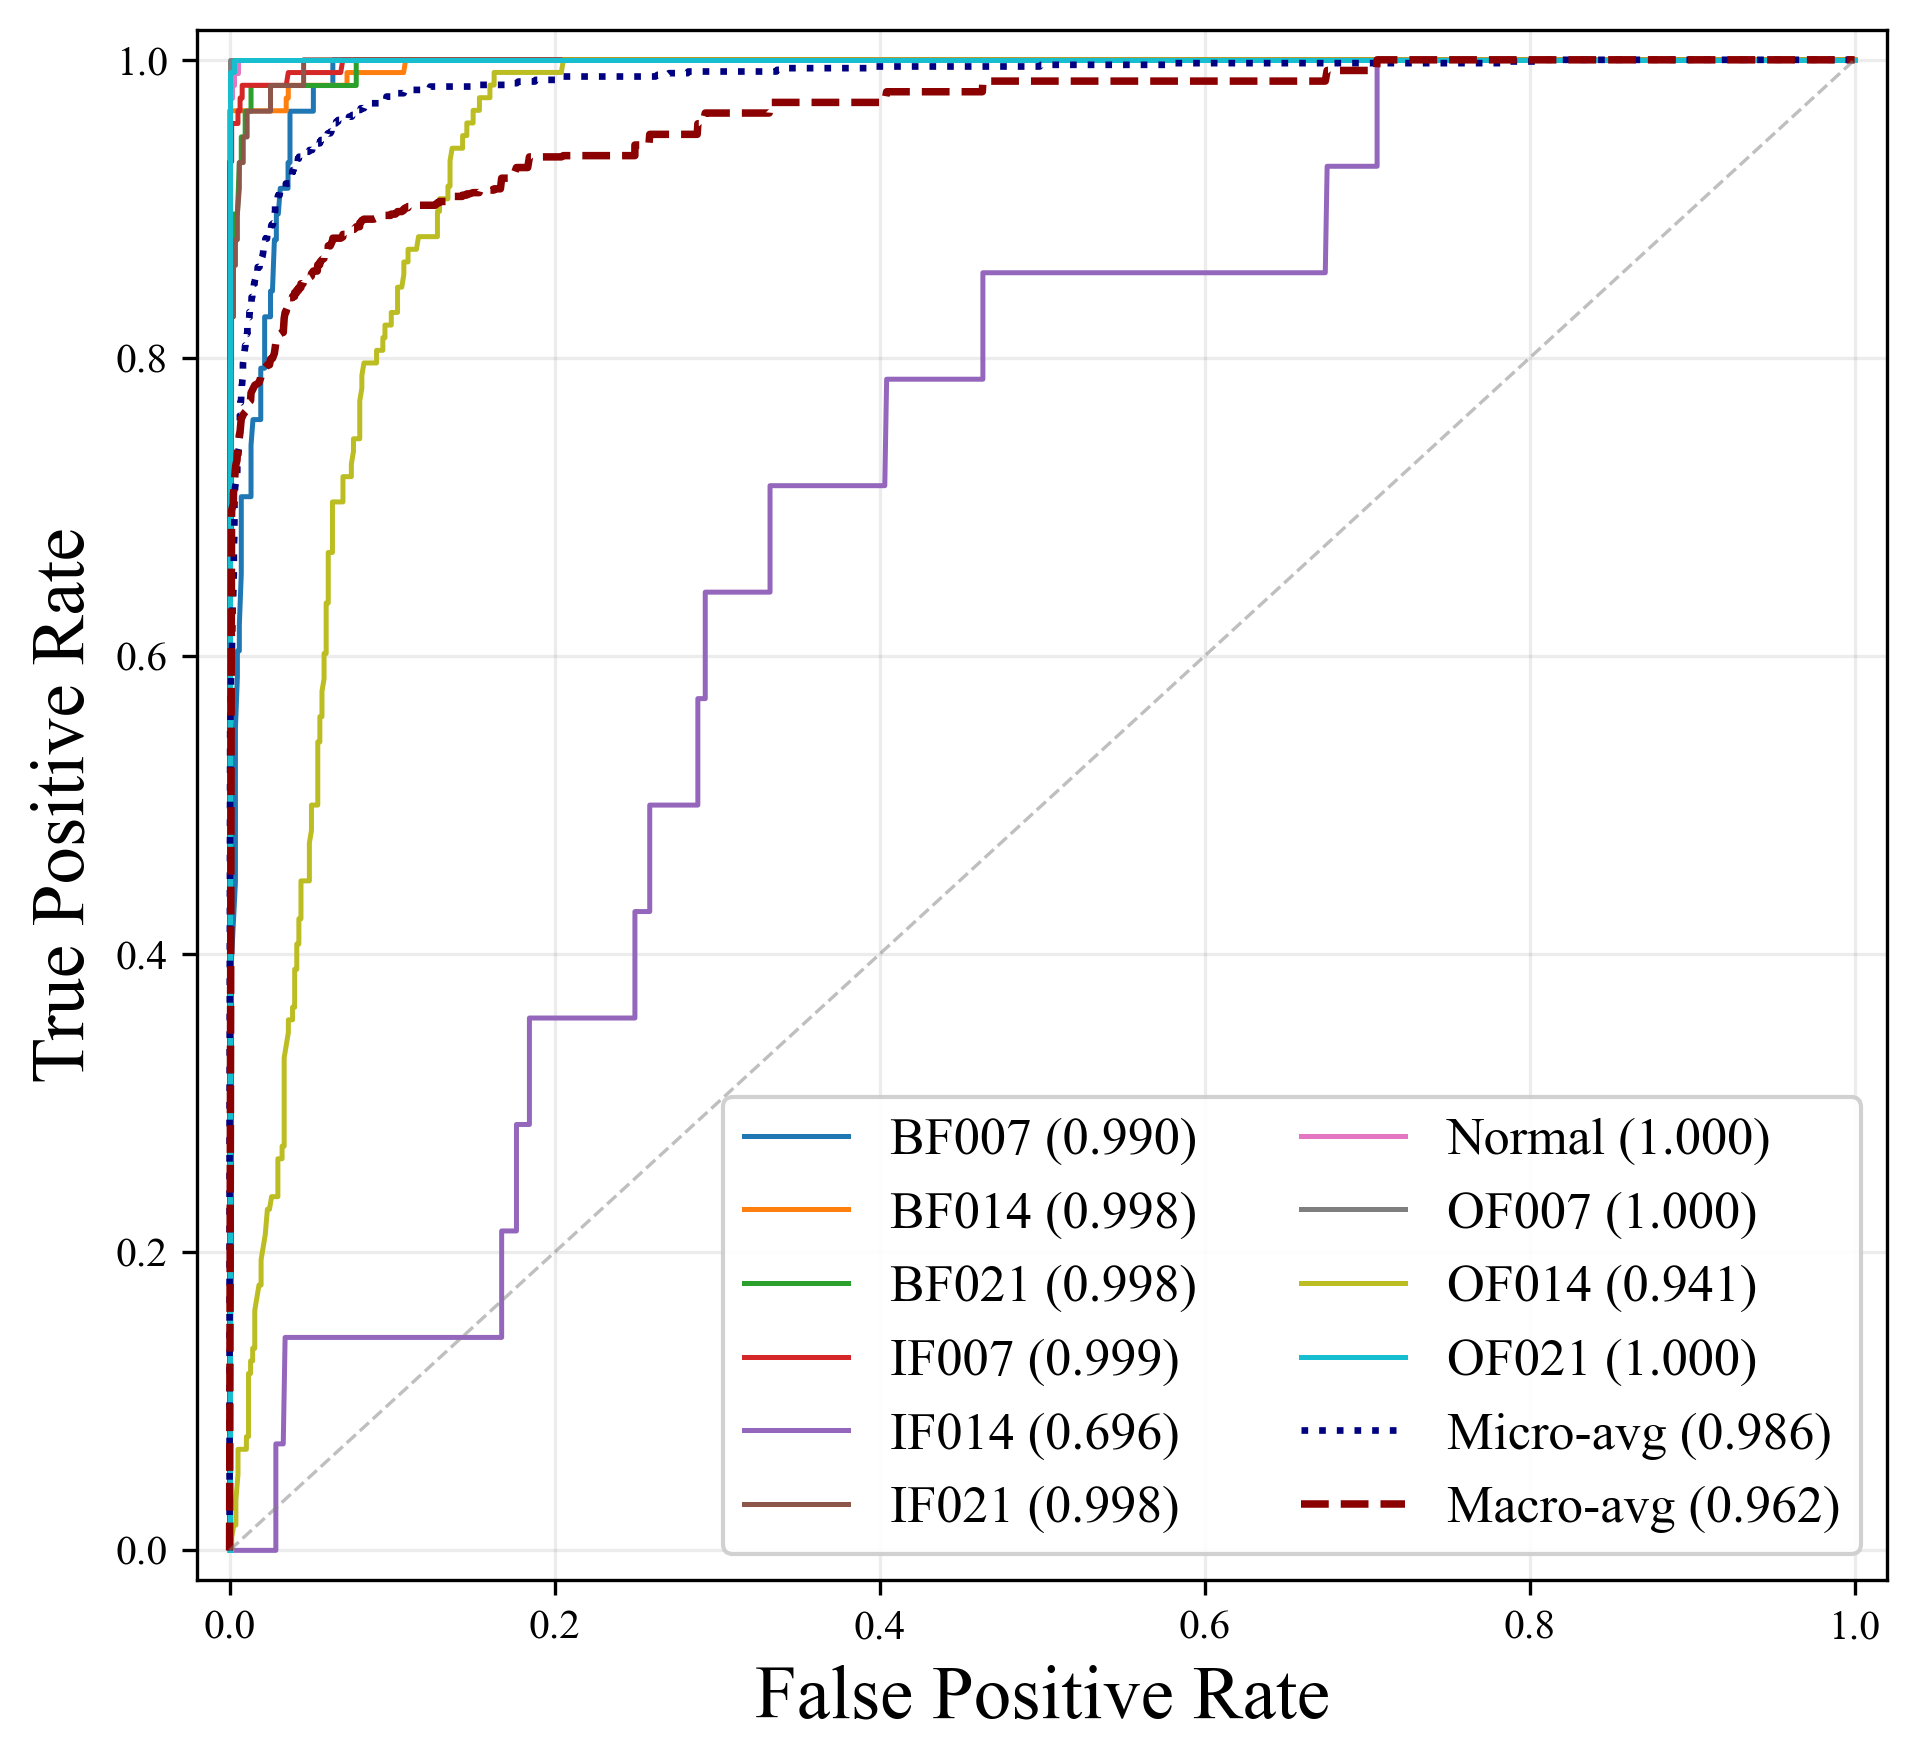
\includegraphics[width=\linewidth]{figures/roc/vit_roc.png}
		\caption{ViT}
	\end{subfigure}
	\hfill
	\begin{subfigure}{0.32\textwidth}
		\centering
		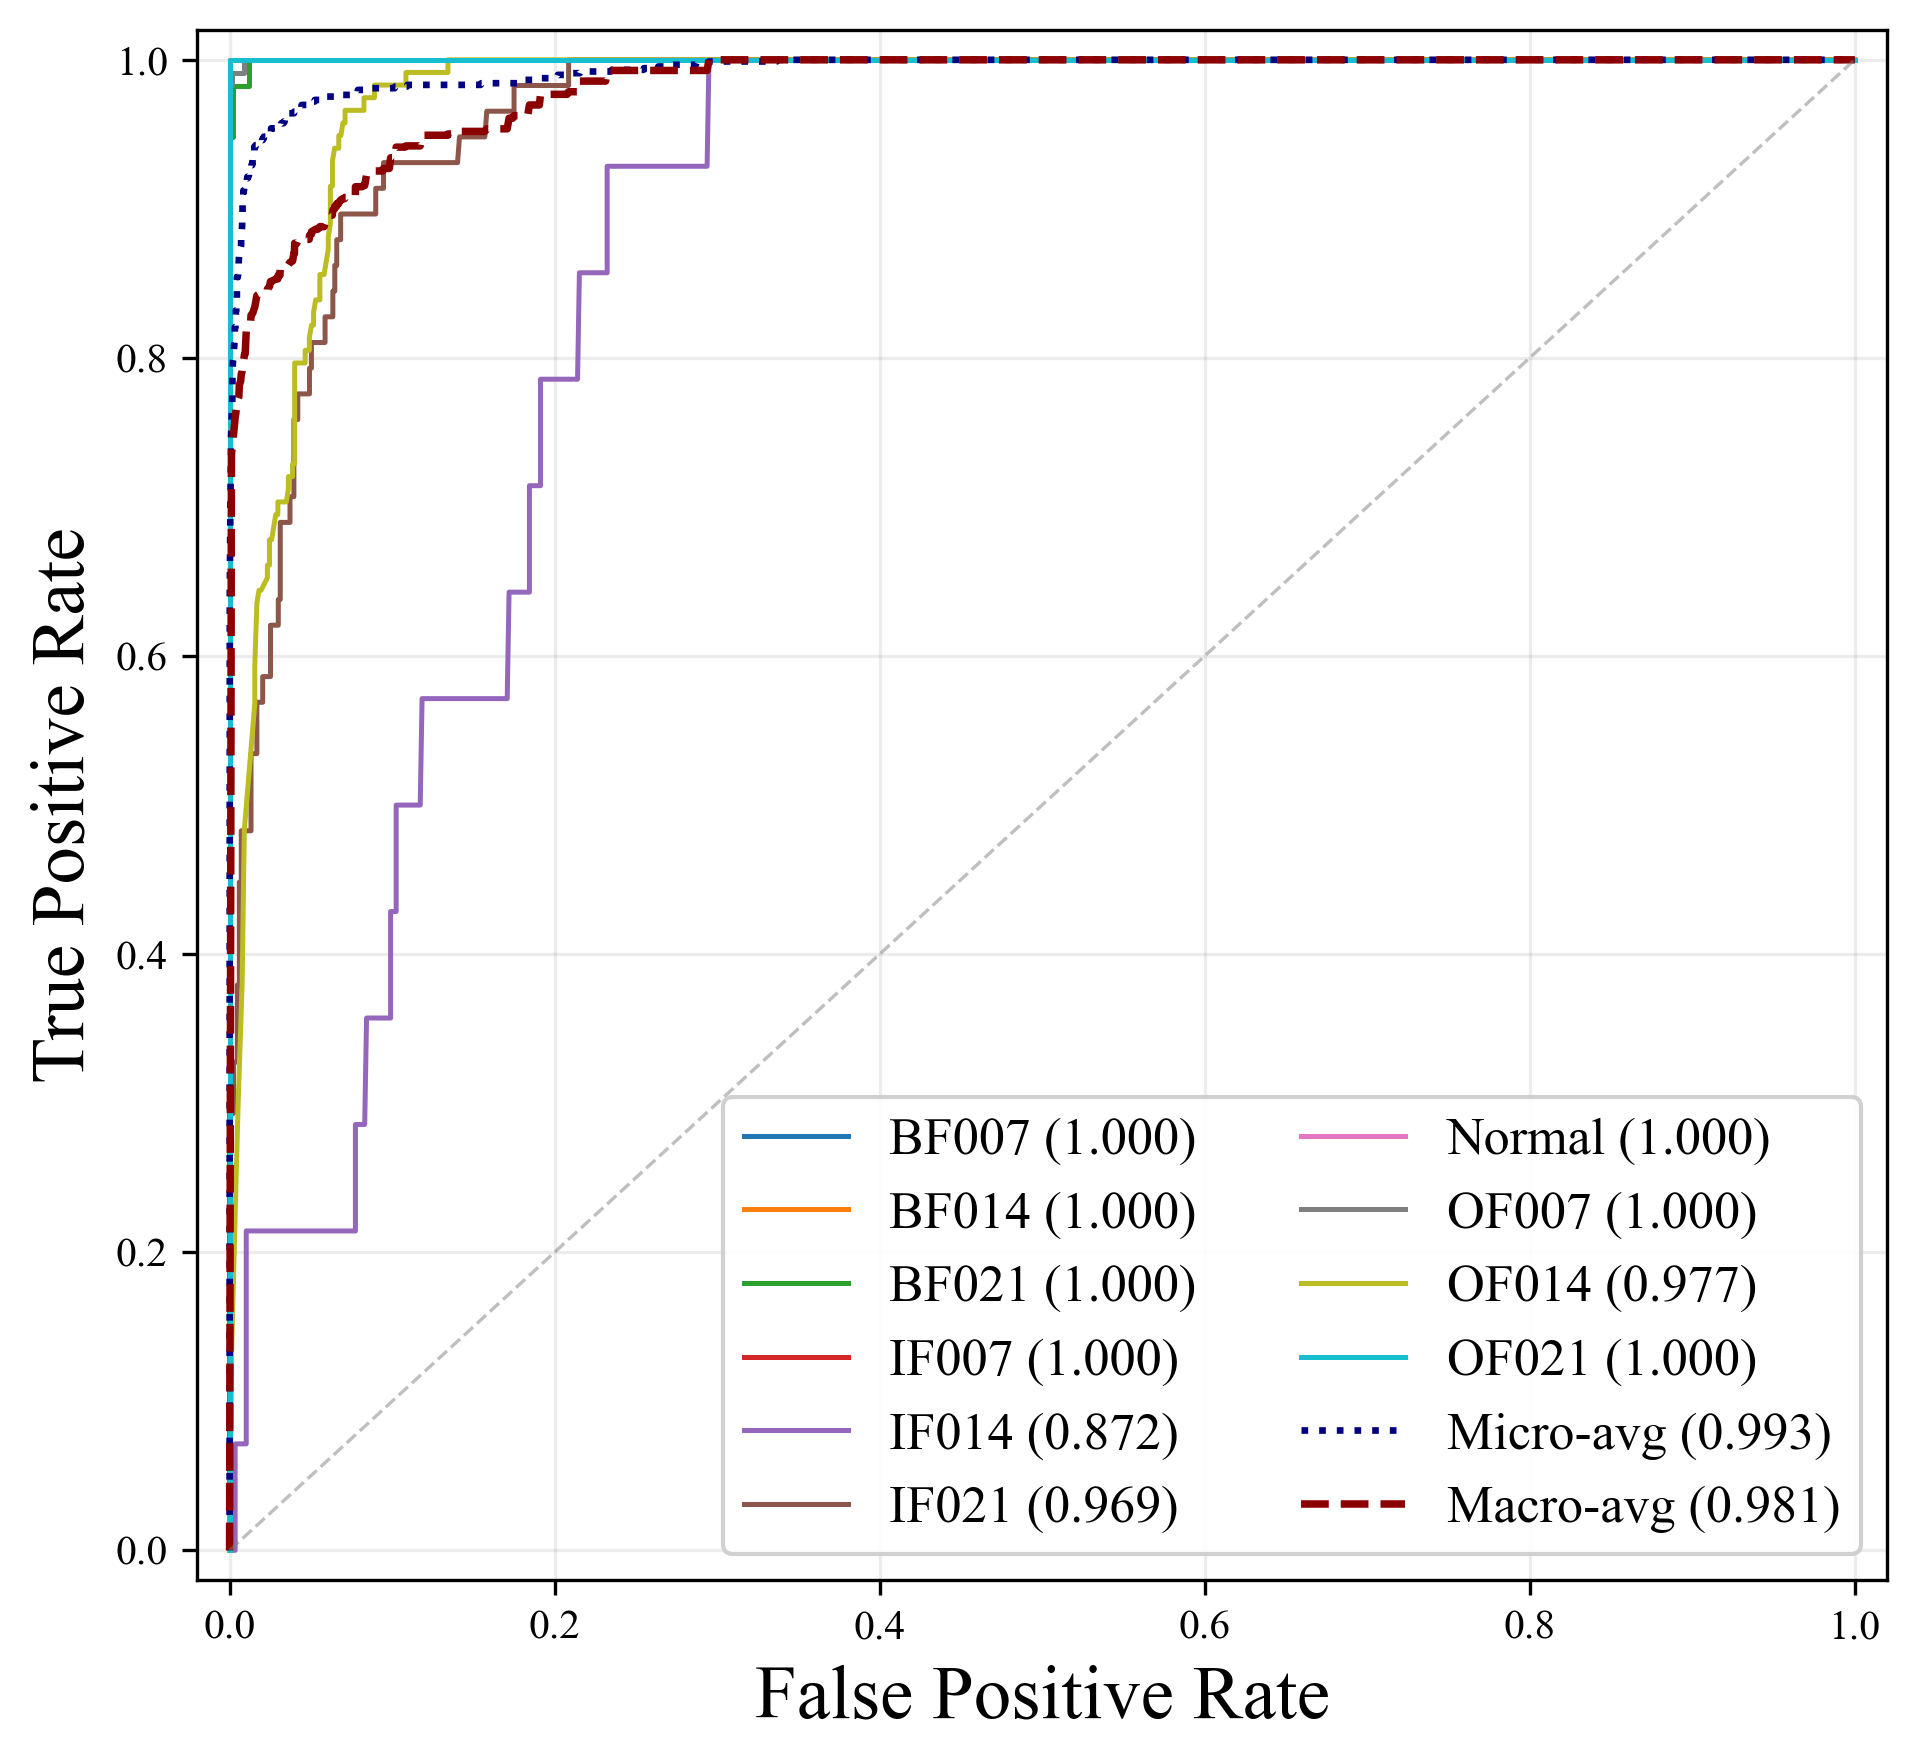
\includegraphics[width=\linewidth]{figures/roc/vgg16_roc.png}
		\caption{VGG16}
	\end{subfigure}

	\vspace{1mm}

	\begin{subfigure}{0.32\textwidth}
		\centering
		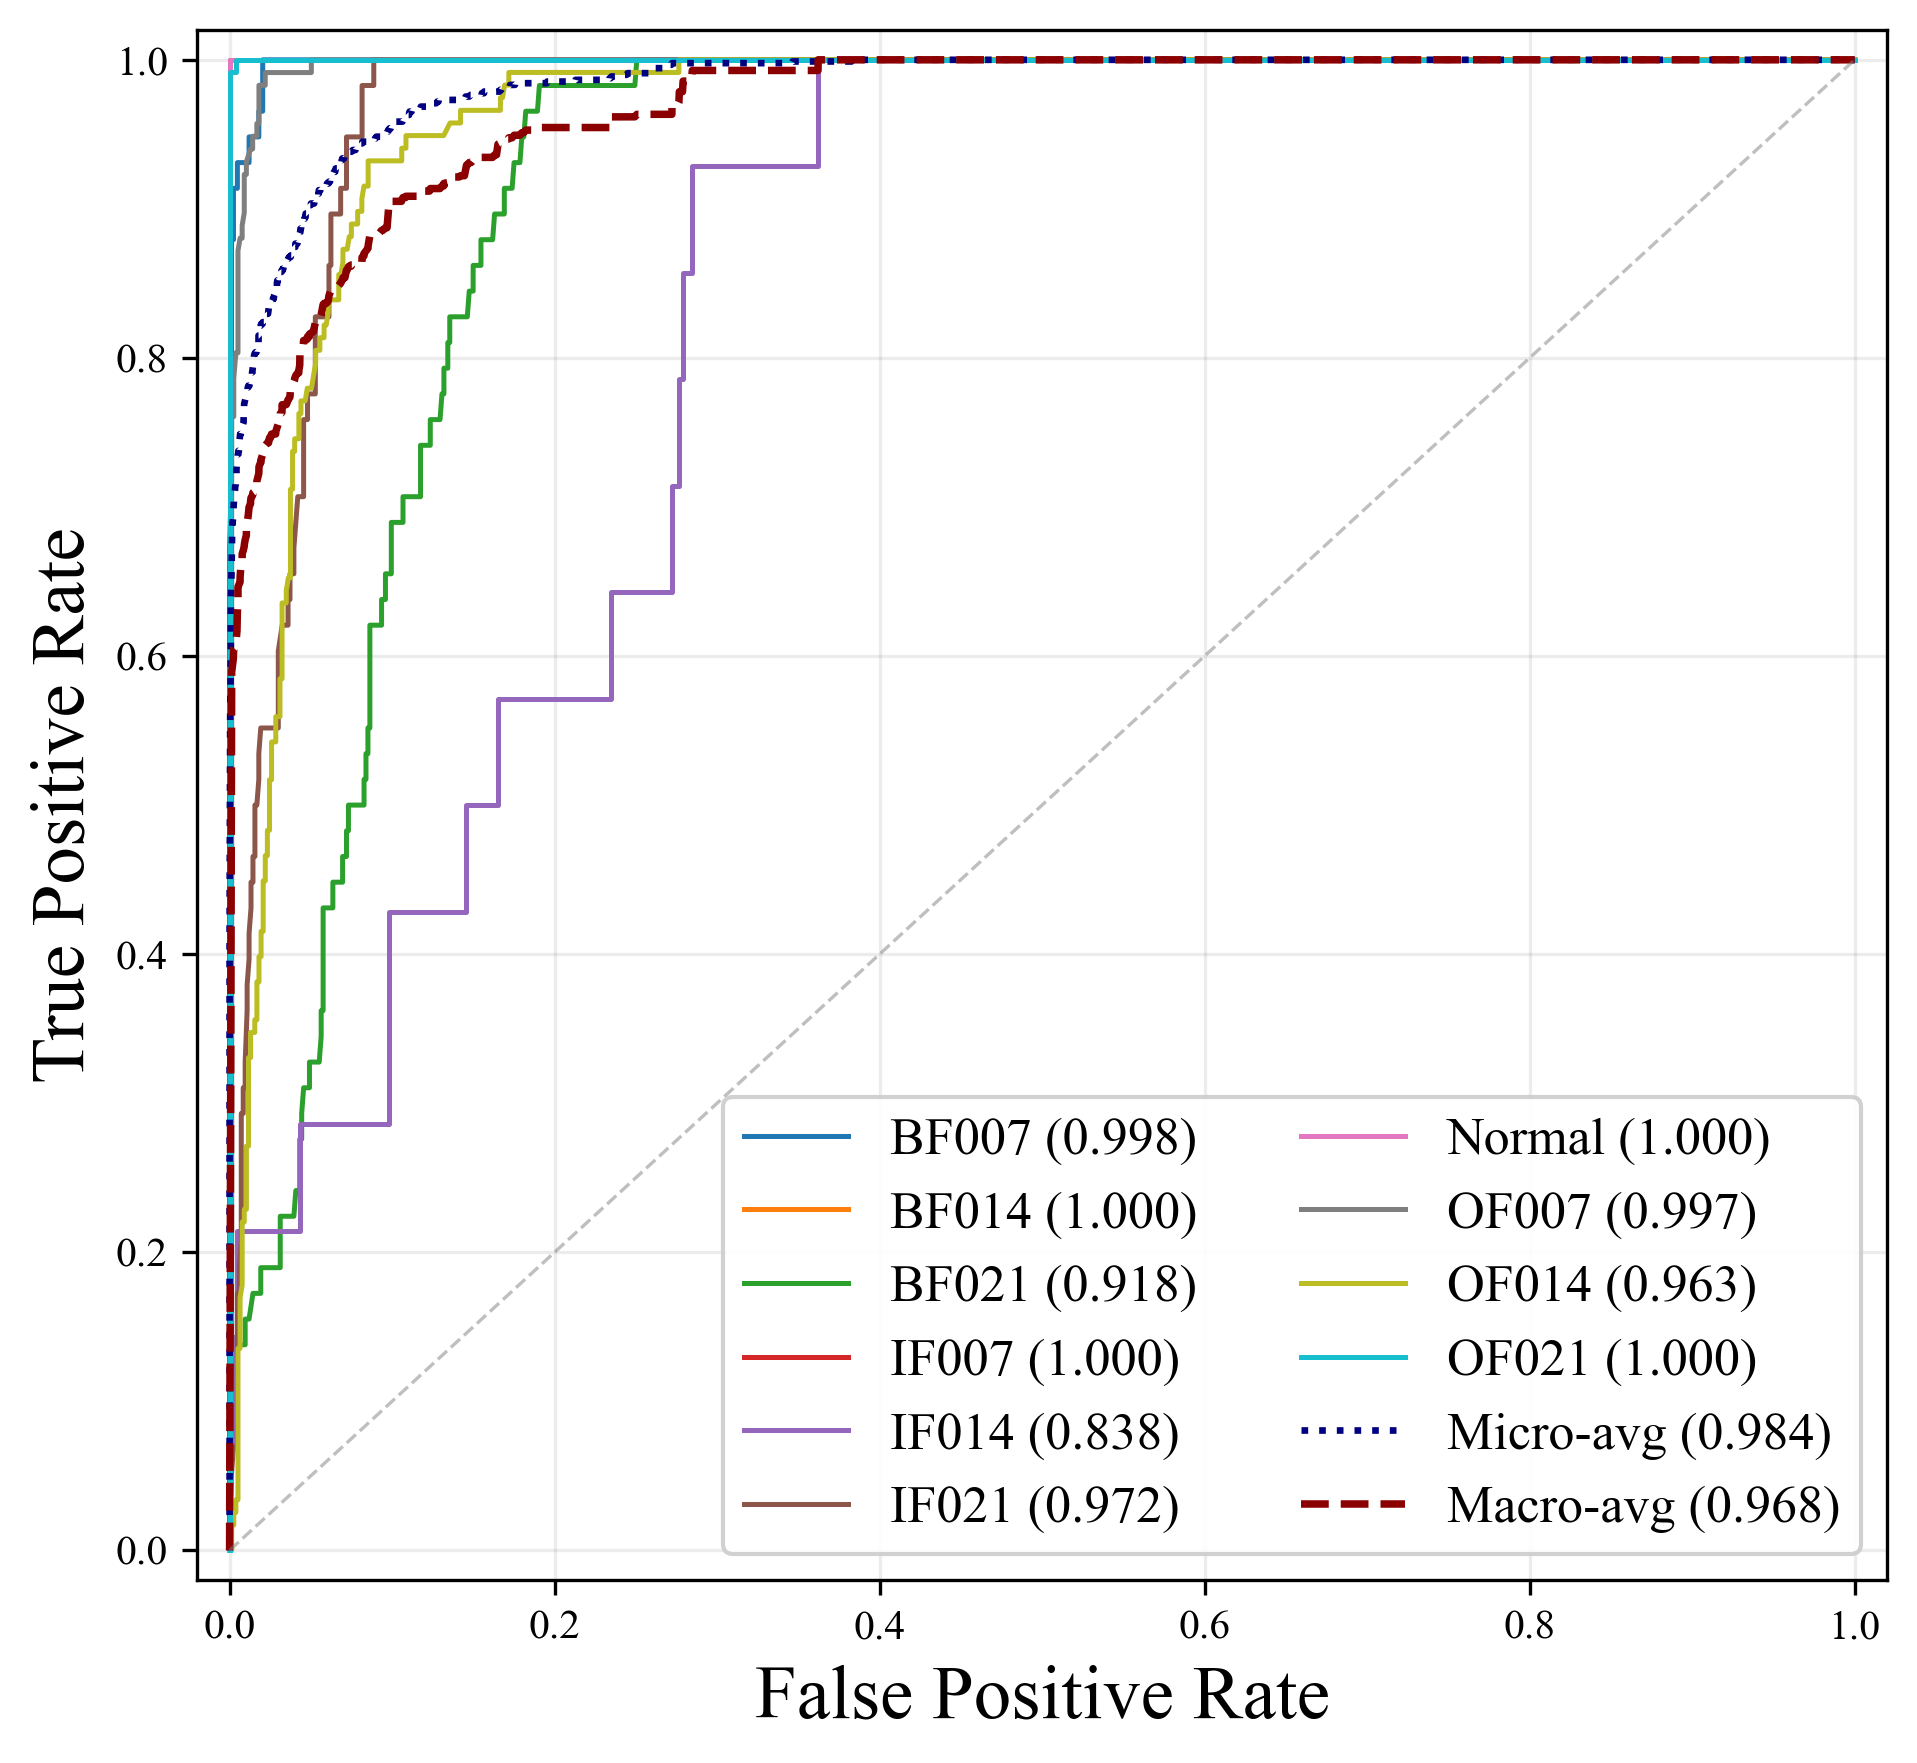
\includegraphics[width=\linewidth]{figures/roc/efficientnet-b0_roc.png}
		\caption{EfficientNet-B0}
	\end{subfigure}
	\hfill
	\begin{subfigure}{0.32\textwidth}
		\centering
		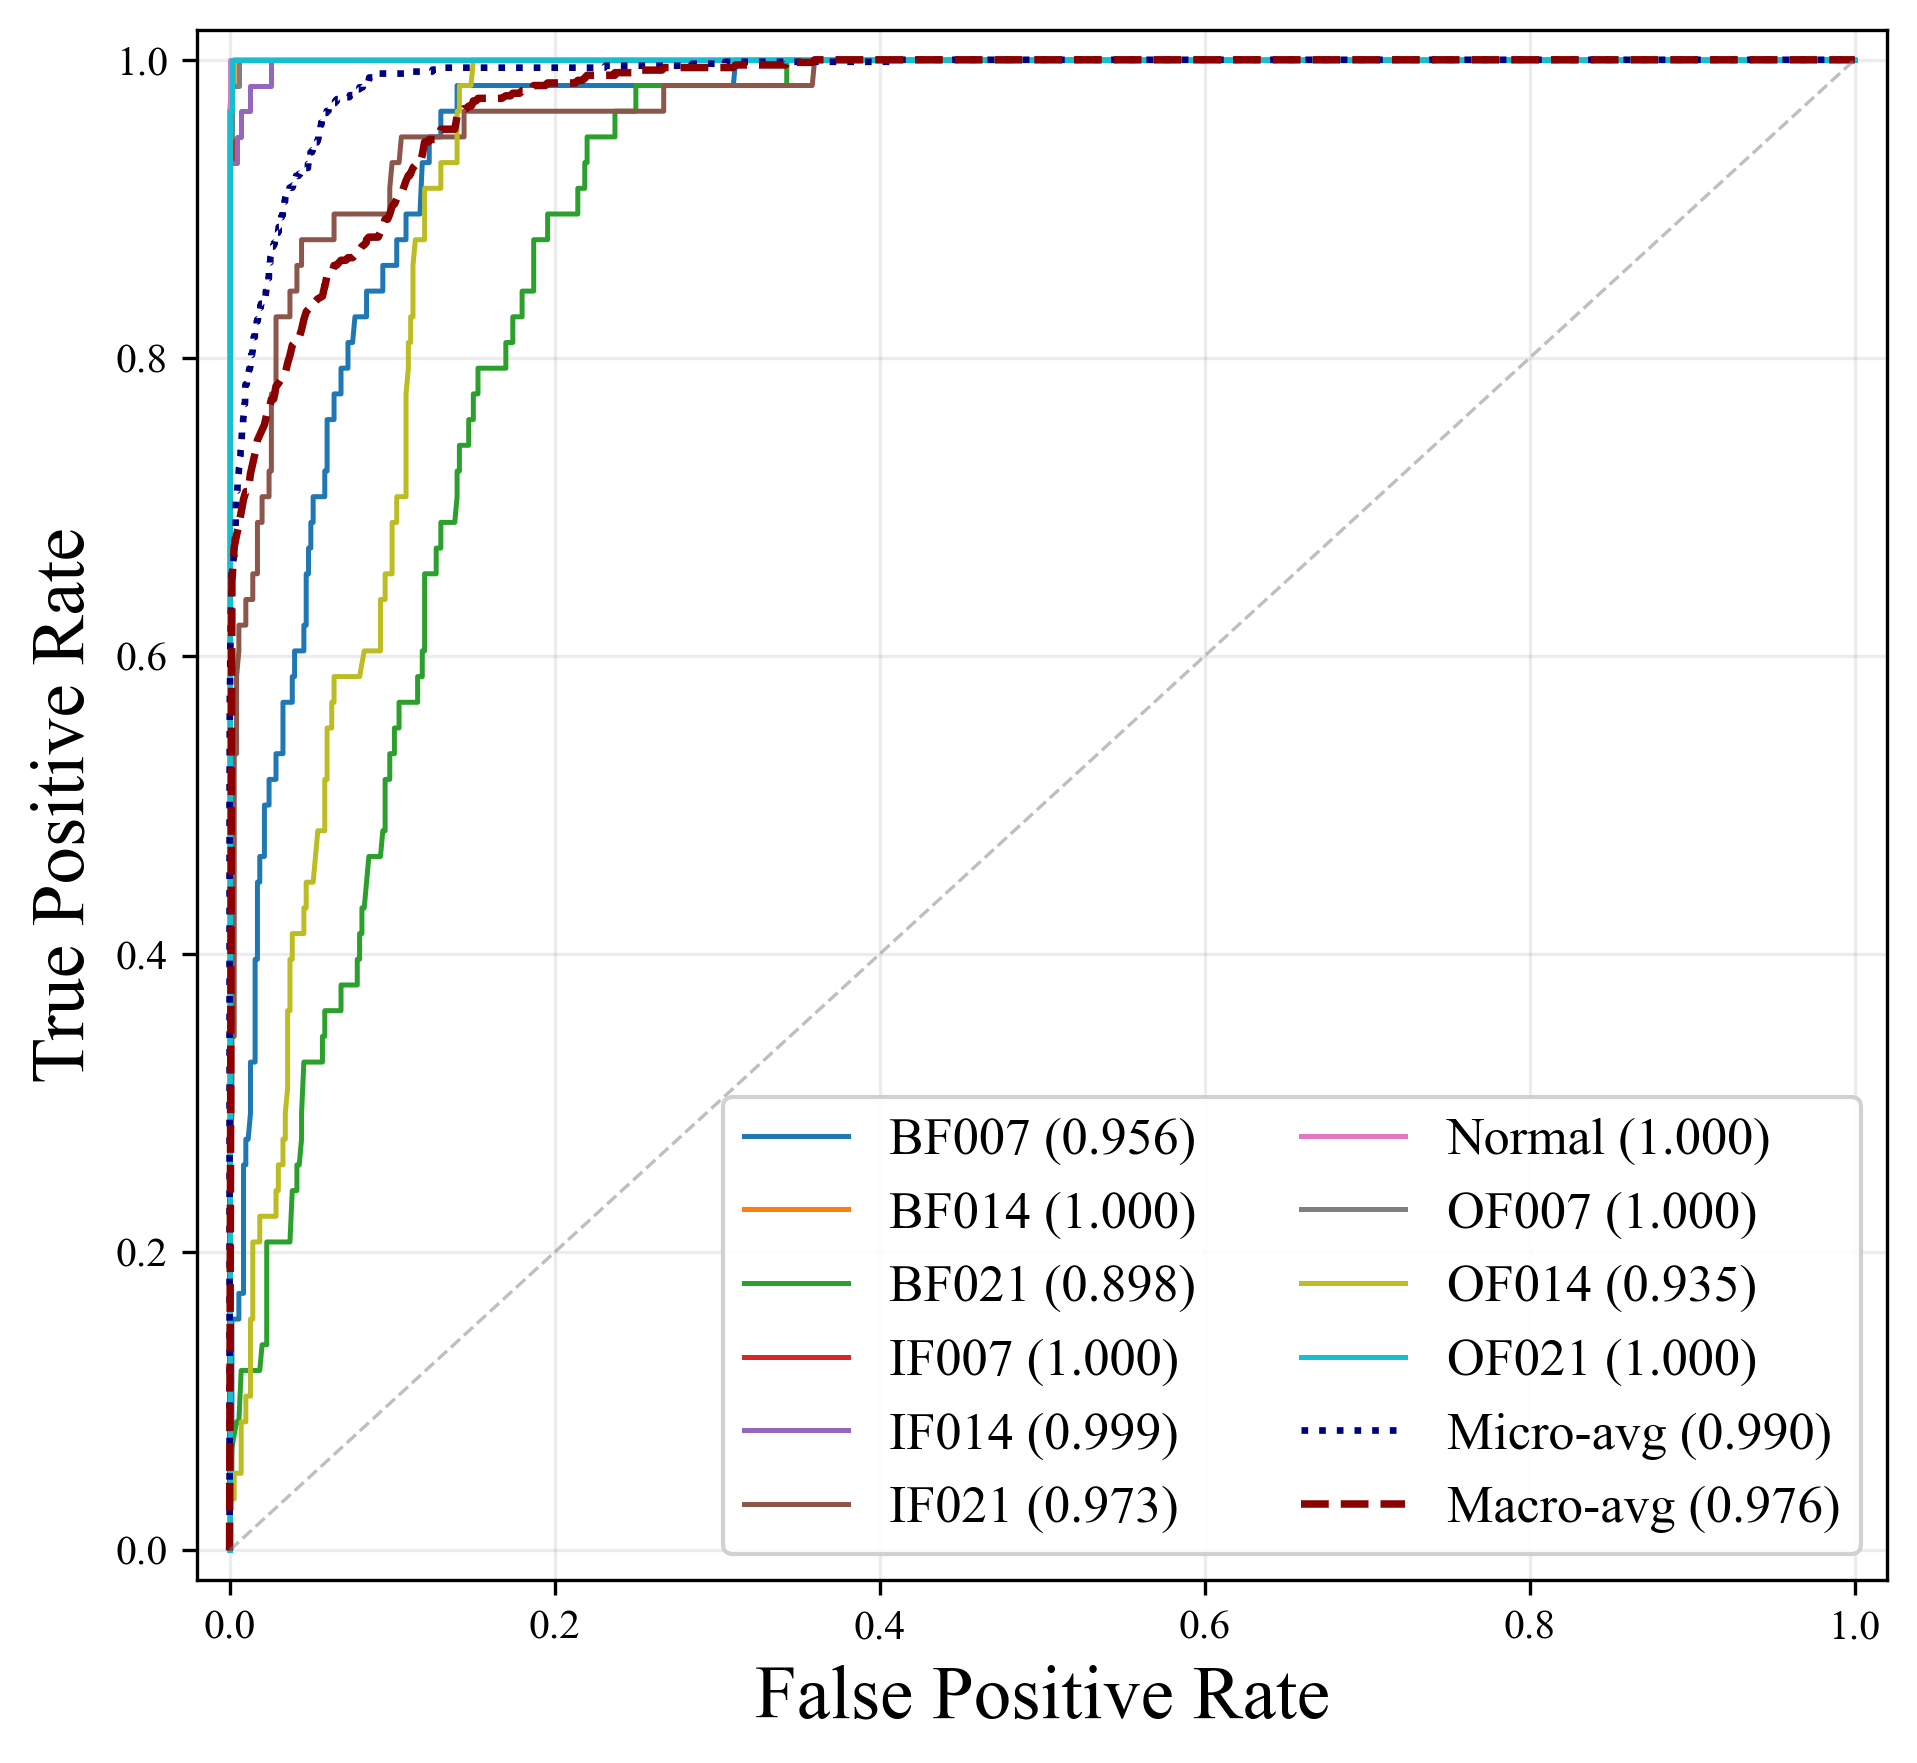
\includegraphics[width=\linewidth]{figures/roc/mobilenetv3_small_roc.png}
		\caption{MobileNetV3-Small}
	\end{subfigure}
	\hfill
	\begin{subfigure}{0.32\textwidth}
		\centering
		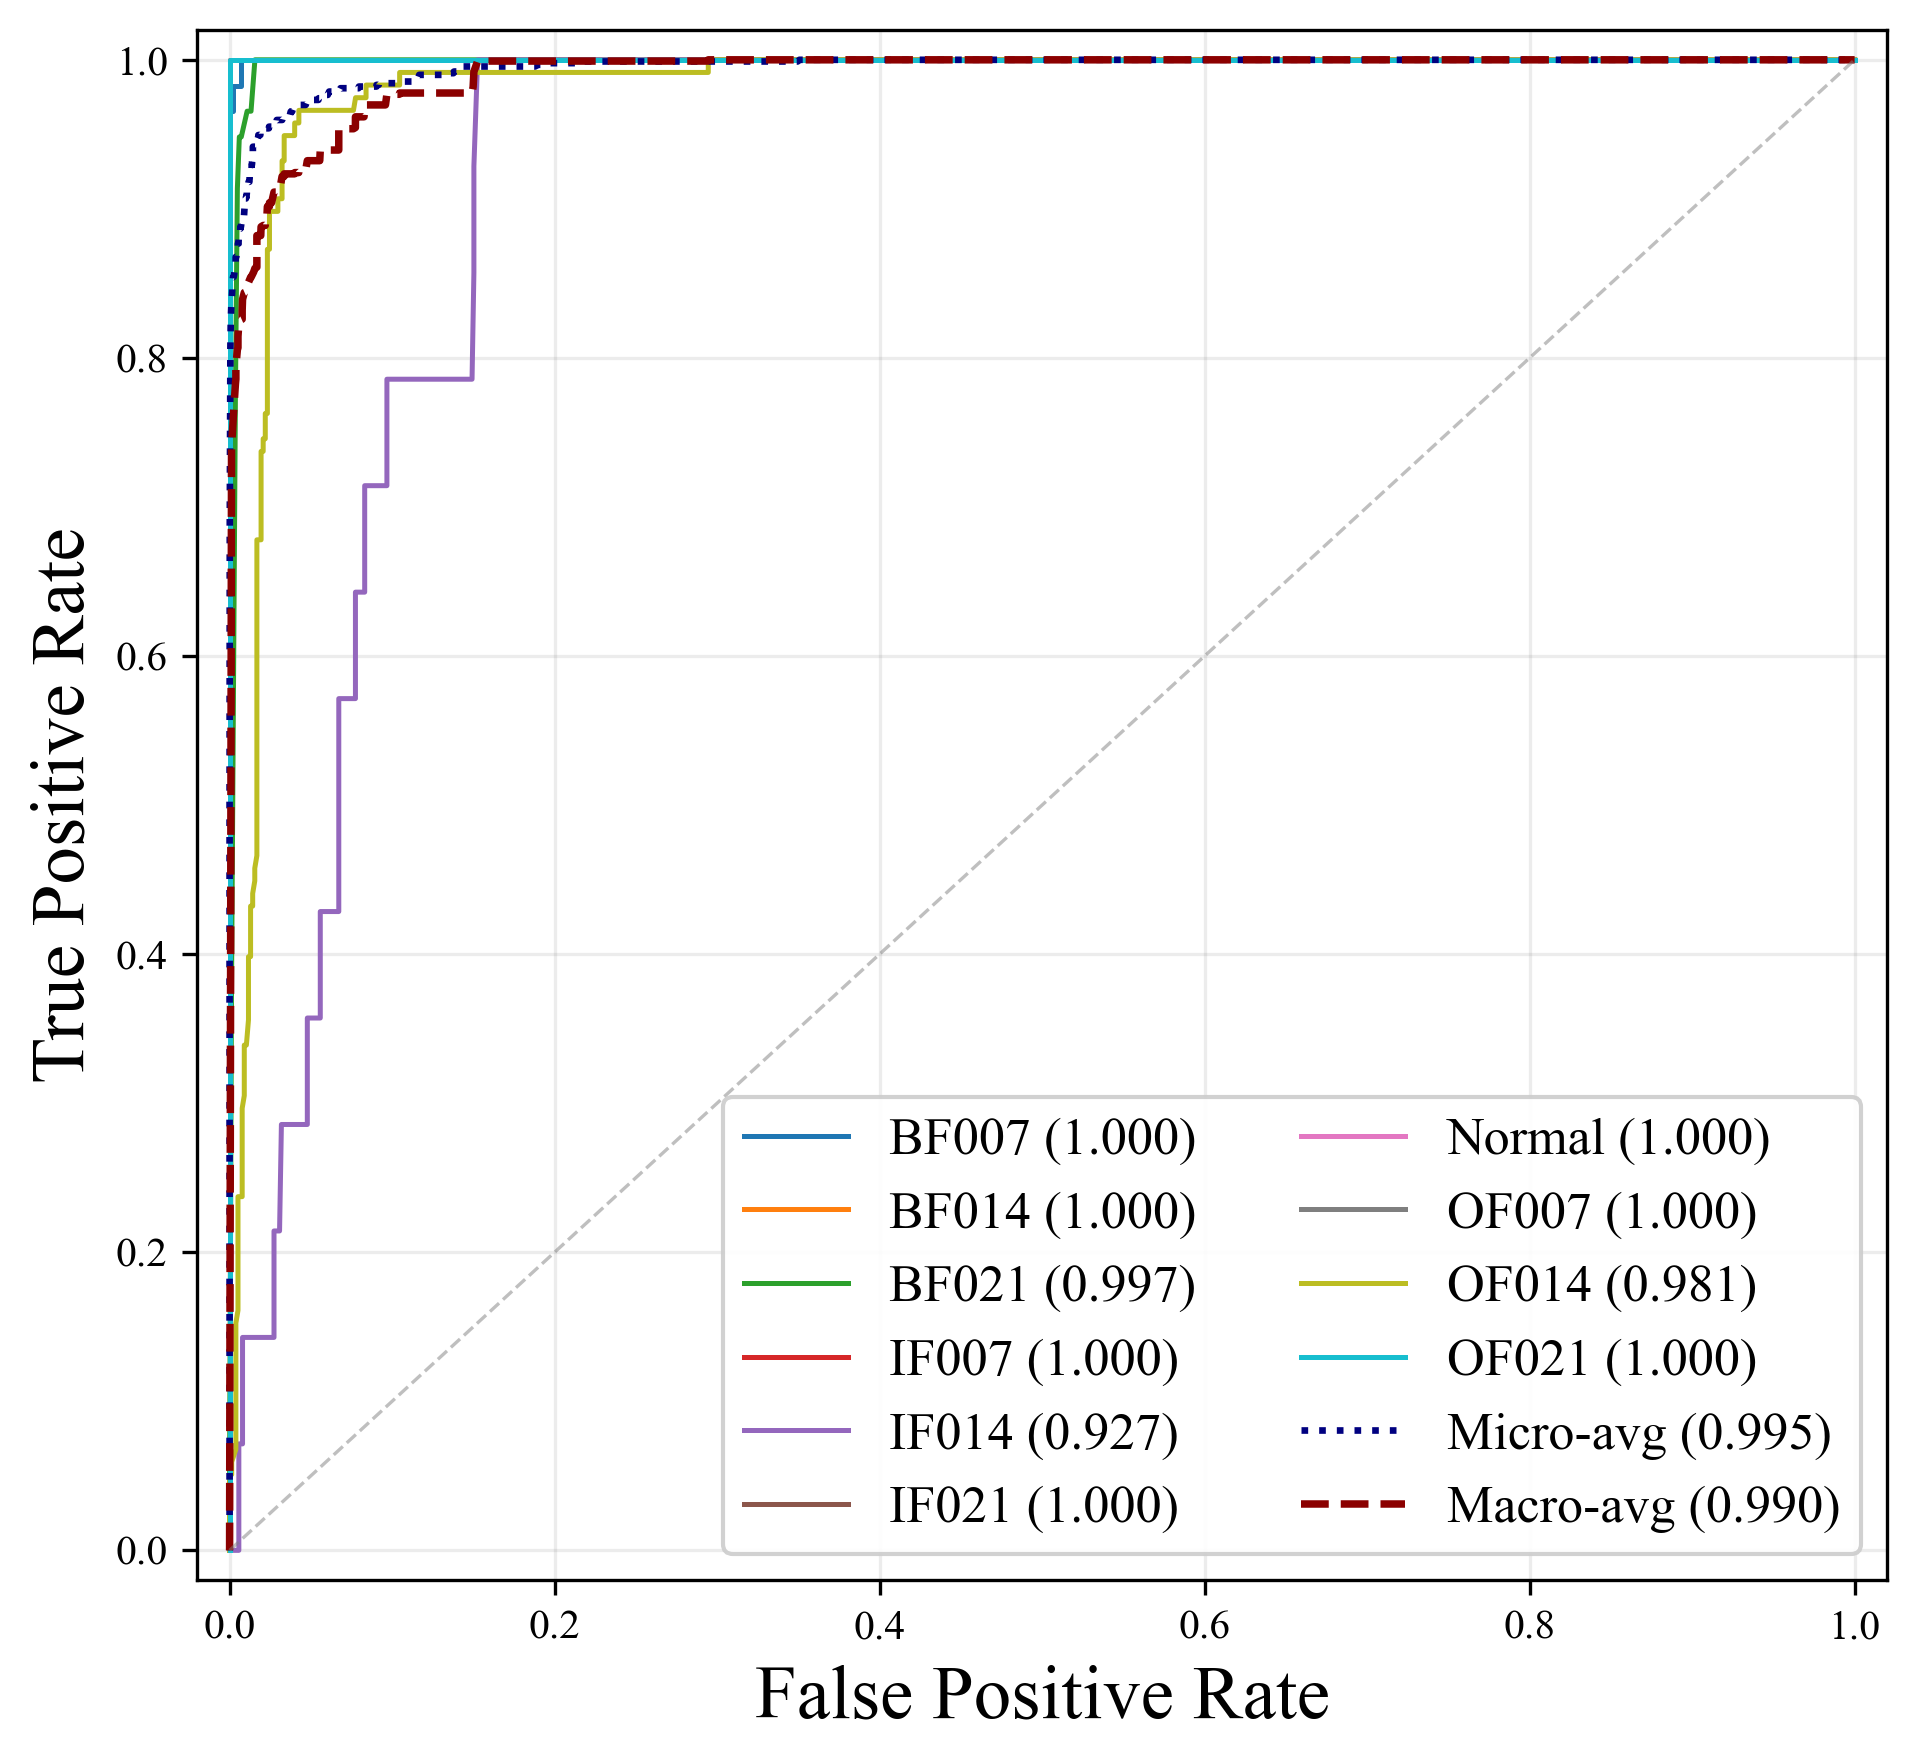
\includegraphics[width=\linewidth]{figures/roc/msca-vgg16_roc.png}
		\caption{MSCA-VGG16 (Ours)}
	\end{subfigure}
	\caption{ROC curves of different backbone networks on the CWRU 12k DE dataset. The proposed MSCA-VGG16 achieves higher AUC on most classes, indicating superior discriminative capability and robustness across classes.}
	\label{fig:roc}
\end{figure*}

% % Auto-generated by scripts/plot_roc_all.py
% Date: 2026-06-29 11:34:44

\begin{table*}[!htbp]
    \centering
    \caption{Per-Class AUC Values Across Backbone Networks.}
    \label{tab:roc_auc}
    \renewcommand{\arraystretch}{1.05}
    \footnotesize
    \begin{tabular}{lccccccc}
        \toprule
        \textbf{Fault Class} & \textbf{MSCA-VGG16 (Ours)} & ConvNeXt-Tiny & EfficientNet-B0 & MobileNetV3-Small & ResNet18 & VGG16 & ViT \\
        \midrule
        BF007 & $\mathbf{1.000}$ & $0.954$ & $0.948$ & $0.969$ & $0.982$ & $0.999$ & $0.990$ \\
        BF014 & $\mathbf{1.000}$ & $0.997$ & $1.000$ & $1.000$ & $1.000$ & $1.000$ & $0.998$ \\
        BF021 & $0.997$ & $0.974$ & $0.971$ & $0.970$ & $\mathbf{1.000}$ & $0.998$ & $0.998$ \\
        IF007 & $\mathbf{1.000}$ & $1.000$ & $1.000$ & $1.000$ & $1.000$ & $1.000$ & $0.999$ \\
        IF014 & $\mathbf{0.927}$ & $0.665$ & $0.650$ & $0.723$ & $0.622$ & $0.738$ & $0.696$ \\
        IF021 & $\mathbf{1.000}$ & $1.000$ & $0.992$ & $0.995$ & $1.000$ & $1.000$ & $0.998$ \\
        Normal & $\mathbf{1.000}$ & $1.000$ & $1.000$ & $1.000$ & $1.000$ & $1.000$ & $1.000$ \\
        OF007 & $\mathbf{1.000}$ & $1.000$ & $1.000$ & $1.000$ & $1.000$ & $1.000$ & $1.000$ \\
        OF014 & $0.981$ & $0.872$ & $0.919$ & $0.939$ & $0.946$ & $\mathbf{0.982}$ & $0.941$ \\
        OF021 & $\mathbf{1.000}$ & $1.000$ & $0.998$ & $1.000$ & $1.000$ & $1.000$ & $1.000$ \\
        \midrule
        \textbf{Macro} & $\mathbf{0.990}$ & $0.946$ & $0.948$ & $0.959$ & $0.955$ & $0.971$ & $0.962$ \\
        \textbf{Micro} & $\mathbf{0.995}$ & $0.975$ & $0.983$ & $0.988$ & $0.988$ & $0.994$ & $0.986$ \\
        \bottomrule
    \end{tabular}
\end{table*}


\subsection{Visualization and Qualitative Analysis}
Qualitative analysis via confusion matrices, ROC curves, and t-SNE visualization corroborates these findings.

\textbf{1) Confusion matrix analysis.} The confusion matrices in Fig.~\ref{fig:confusion_matrix} provide a direct view of per-class classification accuracy and error patterns. MSCA-VGG16 (Fig.~\ref{fig:confusion_matrix}(f)) achieves near-perfect diagonal dominance, with only isolated off-diagonal activations confined to severity-adjacent fault pairs. In comparison, ConvNeXt-Tiny and ViT exhibit diffuse off-diagonal confusion patterns spanning multiple fault types and severities, consistent with their lower quantitative metrics. The progressive diagonal sharpening from lightweight backbones through VGG16 to MSCA-VGG16 visually confirms the cumulative benefit of the proposed architectural enhancements.

\textbf{2) ROC curve analysis.} The ROC curves in Fig.~\ref{fig:roc} provide a threshold-independent assessment of per-class discriminability. MSCA-VGG16 (Fig.~\ref{fig:roc}(f)) achieves near-optimal curves for all ten categories, with macro-averaged AUC approaching unity and minimal false alarm rates across the full decision threshold range. In contrast, ViT (Fig.~\ref{fig:roc}(b)) exhibits the widest inter-class AUC dispersion, ConvNeXt-Tiny (Fig.~\ref{fig:roc}(a)) shows pronounced deterioration on Normal and ball fault classes, and VGG16 (Fig.~\ref{fig:roc}(c)) trails MSCA-VGG16 on severity-adjacent fault pairs where channel attention is critical for fine-grained discrimination. The consistent ROC superiority of MSCA-VGG16 confirms that the multi-scale convolution and channel attention modules jointly enhance per-class discriminability, which is essential for practical deployment where false alarms incur substantial economic cost.

\textbf{3) t-SNE visualization.} The t-SNE projections in Fig.~\ref{fig:tsne_backbones} reveal that raw input pixels exhibit substantial inter-class overlap, confirming that high accuracy is not attributable to inherent input separability. Among all backbones, MSCA-VGG16 produces the most compact, well-separated feature clusters with minimal intra-class dispersion, demonstrating that the proposed multi-scale convolution and channel attention mechanisms effectively transform the AW-DPCNN fused representations into a highly discriminative feature space. Notably, the embedding head's dimensionality reduction contributes to tighter cluster formation for the ball fault and inner race fault categories, which are notoriously challenging to separate due to their similar temporal impulse patterns.


\begin{figure*}[!t]
	\centering
	\begin{subfigure}{0.32\textwidth}
		\centering
		\includegraphics[width=\linewidth]{tsne_cwru_12k_de_raw_input}
		\caption{Raw Input}
	\end{subfigure}
	\hfill
	\begin{subfigure}{0.32\textwidth}
		\centering
		\includegraphics[width=\linewidth]{tsne_vit_12k_de_trial_seed42}
		\caption{ViT}
	\end{subfigure}
	\hfill
	\begin{subfigure}{0.32\textwidth}
		\centering
		\includegraphics[width=\linewidth]{tsne_convnext_tiny_12k_de_trial_seed42}
		\caption{ConvNeXt-Tiny}
	\end{subfigure}

	\vspace{3mm}

	\begin{subfigure}{0.32\textwidth}
		\centering
		\includegraphics[width=\linewidth]{tsne_efficientnet_b0_12k_de_trial_seed42}
		\caption{EfficientNet-B0}
	\end{subfigure}
	\hfill
	\begin{subfigure}{0.32\textwidth}
		\centering
		\includegraphics[width=\linewidth]{tsne_mobilenetv3_small_12k_de_trial_seed42}
		\caption{MobileNetV3-Small}
	\end{subfigure}
	\hfill
	\begin{subfigure}{0.32\textwidth}
		\centering
		\includegraphics[width=\linewidth]{tsne_MSCA_VGG16_12k_de_trial_seed42}
		\caption{MSCA-VGG16 (Ours)}
	\end{subfigure}
	\caption{t-SNE feature visualization of different backbone networks on the CWRU 12k DE bearing test set. The proposed MSCA-VGG16 produces the most compact and well-separated clusters, indicating superior discriminative representation learning.}
	\label{fig:tsne_backbones}
\end{figure*}

% To evaluate the classification performance of the proposed MSCA-VGG16 model, confusion matrices were employed to visualize the recognition accuracy across ten fault categories, as shown in Fig.~\ref{fig:confusion_matrix}. A hierarchical comparison was conducted among the baseline model, several representative deep learning architectures, and the proposed MSCA-enhanced framework. 

% \textbf{1) Performance of the Baseline Model.}
% As illustrated in Fig.~\ref{fig:confusion_matrix}(a), the baseline model exhibits limited capability in distinguishing different transformer operating conditions, particularly harmonic-related conditions. Consequently, multiple harmonic-associated states are frequently misclassified. For example, the recognition accuracy of pure third harmonic category is extremely low, with most samples incorrectly classified as pure fifth harmonic category. In addition, the 30\% seventh harmonic category also shows poor performance and is frequently misclassified as pure fifth harmonic category. Similar confusion can be observed between other harmonic conditions, indicating that the baseline network has difficulty capturing subtle spectral differences among harmonic components. These results demonstrate that the baseline architecture lacks sufficient representation capability to effectively discriminate complex acoustic patterns in transformer fault signals.

% \textbf{2) Performance of Standard Deep Architectures.}
% With the adoption of deeper architectures, including AlexNet, ResNet18, ConvNeXt-Tiny, and VGG16 (Fig.~\ref{fig:confusion_matrix}(b)–(e)), the overall diagnostic performance is noticeably improved compared with the baseline model. The confusion matrices show stronger diagonal dominance, indicating enhanced classification capability across most categories. AlexNet achieves high recognition accuracy for several conditions, such as 30\% fifth harmonic category and pure seventh harmonic category, while misclassification of the normal state remains evident. ResNet18 further improves the recognition of certain harmonic categories, particularly 30\% third harmonic category, although different harmonic components remain difficult to distinguish. ConvNeXt-Tiny and VGG16 exhibit relatively balanced performance across most classes but remain limited in distinguishing acoustically similar harmonic patterns. These observations suggest that although deeper networks strengthen representation capability, accurately discriminating highly similar harmonic signals remains challenging for conventional backbone architectures.

% \textbf{3) Superiority of the Proposed MSCA-VGG16 Model.}
% As shown in Fig.~\ref{fig:confusion_matrix}(f), the proposed MSCA-VGG16 model achieves the most consistent and accurate classification results among all evaluated architectures. By incorporating the Multi-Scale Convolutional Attention (MSCA) mechanism, the model effectively enhances discriminative representation and suppresses inter-class confusion. Several categories, including 10 kV overload, loosen, partial discharge, and pure seventh harmonic, are recognized with perfect accuracy. Moreover, the recognition performance of previously challenging harmonic-related conditions is significantly improved. For example, the accuracy of the 30\% seventh harmonic category increases to 62\%, while the 30\% third harmonic category reaches 99\% accuracy. Although slight confusion still exists between pure third harmonic and pure fifth harmonic category, the overall confusion pattern is substantially reduced compared with the other backbone networks. These results indicate that the proposed MSCA-VGG16 framework provides more discriminative acoustic representation learning and achieves superior robustness for transformer acoustic fault diagnosis.

% Auto-generated by scripts/analyze_results.py
% Date: 2026-06-26 11:54:03
% These tables can be \input{} directly into tim.tex
% ── Ablation Table (B0–B8) ──
\begin{table*}
    \centering
    \caption{Unified Component Decomposition Ablation (B0–B8, Mean $\pm$ Std over 3 Independent Trials). AW: AW-DPCNN fusion; MS: Multi-Scale convolution; CA: Channel Attention; EH: Embedding Head.}
    \label{tab:ablation_unified}
    \renewcommand{\arraystretch}{1.15}
    \small
    \begin{tabular}{lcccccccc}
        \toprule
        \textbf{Exp.} & \textbf{AW-DPCNN} & \textbf{MS} & \textbf{CA} & \textbf{EH} & \textbf{Acc (\%)} & \textbf{F1 (\%)} & \textbf{G-mean (\%)} & \textbf{Kappa (\%)} \\
        \midrule
        \multicolumn{9}{c}{\textit{Fusion-level ablation (VGG16 classifier)}} \\
        B0 & $\times$ & $\times$ & $\times$ & $\times$ & $97.97 \pm 3.05$ & $97.47 \pm 3.88$ & $96.80 \pm 5.02$ & $97.73 \pm 3.42$ \\
        B1 & $\times$ & $\times$ & $\times$ & $\times$ & $58.53 \pm 2.71$ & $56.55 \pm 3.40$ & $12.33 \pm 1.30$ & $54.23 \pm 3.05$ \\
        B2 & $\times$ & $\times$ & $\times$ & $\times$ & $97.87 \pm 3.63$ & $98.01 \pm 3.37$ & $98.15 \pm 3.14$ & $97.62 \pm 4.05$ \\
        B3 & $\checkmark$ ($\gamma$=1) & $\times$ & $\times$ & $\times$ & $89.21$ & $85.99$ & $74.32$ & $87.92$ \\
        B4 & $\checkmark$ ($\gamma$=10) & $\times$ & $\times$ & $\times$ & $95.30$ & $94.43$ & $92.98$ & $94.73$ \\
        \midrule
        \multicolumn{9}{c}{\textit{Classifier-level ablation (full AW-DPCNN fusion)}} \\
        B5 & $\checkmark$ & $\checkmark$ & $\times$ & $\times$ & $99.85$ & $99.83$ & $99.83$ & $99.83$ \\
        B6 & $\checkmark$ & $\times$ & $\checkmark$ & $\times$ & $95.92$ & $95.36$ & $94.81$ & $95.42$ \\
        B7 & $\checkmark$ & $\times$ & $\times$ & $\checkmark$ & $98.23$ & $98.03$ & $97.86$ & $98.01$ \\
        \textbf{B8} & $\checkmark$ & $\checkmark$ & $\checkmark$ & $\checkmark$ & $\mathbf{99.46}$ & $\mathbf{99.41}$ & $\mathbf{99.39}$ & $\mathbf{99.40}$ \\
        \bottomrule
    \end{tabular}
\end{table*}

% % ── Comparison with Previous Works in I&M Journals ──
% References marked with [TODO] should be added manually by the user.
\begin{table*}[!t]
\caption{Performance Comparison Between the Proposed Method and Representative Works Published in I\&M Journals\label{tab:previous_works}}
\centering
\renewcommand{\arraystretch}{1.15}
\footnotesize
\setlength{\tabcolsep}{3.5pt}
\begin{tabular}{c c l l c c p{3.8cm}}
\toprule
\textbf{Ref.} & \textbf{Year} & \textbf{Method} & \textbf{Input} & \textbf{Acc. (\%)} & \textbf{F1 (\%)} & \textbf{Remarks} \\
\midrule
\multicolumn{7}{c}{\textit{IEEE Transactions on Instrumentation and Measurement}} \\
\midrule
\cite{9440949}  & 2021 & SVM + info. fusion      & Vibration \& current & --   & --   & Wind turbine gearbox; traditional ML \\
\cite{8853278}  & 2020 & Mean shift clustering   & Raw vibration        & --   & --   & Unsupervised; gearbox, not bearing \\
\cite{8788665}  & 2020 & CNN + decision fusion   & Motor current        & --   & --   & Current-based; CWRU, not vibration \\
\cite{11028059} & 2025 & Contrastive learning    & Vibration (STFT)     & --   & --   & Open-set; semi-supervised \\
\cite{10929672} & 2025 & GAN + multi-label CNN   & Acoustic (Mel)       & --   & --   & Acoustic; compound faults \\
\cite{11345448} & 2026 & Log-Gabor network       & Raw vibration        & --   & --   & Single rep.; no fusion \\
\midrule
\multicolumn{7}{c}{\textit{Other I\&M journals --- CWRU bearing (vibration)}} \\
\midrule
\cite{YI2025116881}    & 2025 & VibrMamba              & Raw vibration (1-D)  & 99.77 & --   & Lightweight SSM; no TF fusion \\
\cite{ZHANG2026106301} & 2026 & PCA-RAM + CBAM-CNN      & GAF image            & 99.50 & --   & Single encoding; 5-class task \\
\cite{10663388}        & 2025 & MobileViT + deconv.     & MTF image            & --    & --   & Anti-noise; single rep. \\
\cite{DUAN2026122469}  & 2026 & ResNet18-SimAM          & MTF image            & 98.11 & 98.11& FBG sensor; gearbox \\
\midrule
\multicolumn{7}{c}{\textit{This work}} \\
\midrule
\textbf{Ours} & 2026 & \textbf{AW-DPCNN + MSCA-VGG16} & \textbf{STFT + GADF} & $\mathbf{99.85 \pm 0.10}$ & $\mathbf{99.46 \pm 0.43}$ & Multi-rep. fusion; multi-scale attn.; 10-class; cross-sensor \& rate \\
\bottomrule
\end{tabular}
\end{table*}


\subsection{Ablation Study}
\label{sec:ablation}

To isolate the contribution of each component, a systematic ablation study comprising eight configurations (B0--B7) is conducted in two tiers, i.e., B0--B3 examine the fusion pipeline with a standard VGG16 classifier to isolate representation-level effects; B4--B7 build upon the full AW-DPCNN fusion to evaluate individual MSCA-VGG16 components. All configurations use identical training settings (AdamW, $\eta=1\times10^{-4}$, batch size 32, 30 epochs) and are evaluated over three independent trials reported as mean $\pm$ standard deviation. Table~\ref{tab:ablation_unified} reports the results. Key findings are listed as follows.

\textbf{1) Fusion-level ablation (B0--B3).} The single-representation baselines establish performance bounds, i.e., B0 (STFT-only) achieves 93.37\% accuracy, whereas B1 (GADF-only) reaches only 60.99\%, confirming that temporal encoding alone lacks the frequency-domain specificity required for fine-grained fault classification. The naive concatenation strategy B2 improves accuracy to 96.28\%, indicating complementary information between the two representations, but the high standard deviation ($\pm 4.49\%$) reveals instability from destructive interference. AW-DPCNN fusion (B3) achieves 96.30\% accuracy with dramatically reduced variance ($\pm 0.49\%$), demonstrating that while AW-DPCNN does not substantially boost peak accuracy over concatenation at the fusion tier, it provides robust stabilization by adaptively regulating cross-representation contributions.

\textbf{2) Classifier-level ablation (B4--B7).} Using AW-DPCNN fusion as the fixed representation baseline (B3, 96.30\%), MSCA-VGG16 components are evaluated incrementally. Multi-scale convolution alone (B4, with MS) yields a marginal gain to 96.84\% but reintroduces high variance ($\pm 4.01\%$), suggesting that unguided multi-scale processing introduces feature redundancy. Channel attention (B5, with CA) provides the largest single-component improvement, boosting accuracy to 98.97\% (an increase of 2.67\%), confirming that dynamic frequency-band recalibration effectively emphasizes fault-discriminative channels. The compact embedding head (B6, with EH) achieves 98.10\%, a moderate improvement. The full MSCA-VGG16 (B7, combining MS, CA, and EH) attains 99.85\% accuracy with the tightest standard deviation ($\pm 0.10\%$), demonstrating that the three modules function synergistically, i.e., CA drives discriminative channel selection, while MS and EH provide complementary regularization that collectively stabilizes training.

\textbf{3) Cumulative decomposition.} From B1 (GADF-only, 60.99\%) to B7 (full model, 99.85\%), the total gain of 38.86\% decomposes as follows. The STFT representation provides the foundational spectral discrimination (32.38\%, from B1 to B0); AW-DPCNN fusion contributes robust integration (2.93\% over STFT-only, from B0 to B3); and the MSCA-VGG16 classifier adds 3.55\% (from B3 to B7), with channel attention accounting for the majority of this gain.

% \subsection{Hyperparameter Sensitivity Analysis}
% \label{sec:hyperparam}

% The AW-DPCNN fusion module involves several key hyperparameters whose settings may influence the quality of the fused representation and, consequently, the downstream classification performance. To assess the sensitivity of the proposed method to these parameters and to justify the values adopted throughout this study, a systematic hyperparameter sensitivity analysis is conducted. Three critical parameters are examined: the contrast amplification factor $\gamma$, which controls the degree of emphasis placed on the dominant representation in the adaptive weighting scheme; the number of PCNN iterations $N$, which governs the depth of pulse-coupled interaction; and the decay coefficients $\alpha_L$ and $\alpha_T$, which regulate the temporal dynamics of the linking field and the firing threshold, respectively. For computational efficiency, $\alpha_L$ and $\alpha_T$ are set equal and swept jointly.

% For each parameter configuration, the raw test-set acoustic windows are re-fused on-the-fly using the AW-DPCNN module with the specified parameter values, while keeping all other parameters at their default settings ($\gamma=10$, $N=20$, $\alpha_L=\alpha_T=0.001$). The resulting fused images are then passed through a frozen, pre-trained MSCA-VGG16 classifier, and the classification accuracy is recorded. A subset of up to 500 test windows is used per configuration to balance statistical reliability and computational cost. Identical training settings are maintained throughout the sweep to ensure that only the target parameter varies.     

% Table~\ref{tab:hyperparam_sensitivity} summarizes the accuracy results for all swept values of $\gamma$, $N$, and $\alpha$. Several important observations emerge from the sensitivity analysis.

% \textbf{1) Contrast amplification factor $\gamma$.} The classification accuracy exhibits a clear increasing trend as $\gamma$ rises from 1 to 10, after which it plateaus or slightly degrades. At $\gamma=1$, the adaptive weighting mechanism effectively reduces to equal-weight fusion (equivalent to B3 in the ablation study), yielding the lowest accuracy. As $\gamma$ increases, the STFT representation, which carries richer fault-discriminative information in the time--frequency domain, receives progressively greater emphasis, leading to improved performance. The optimal range is $\gamma \in [8, 10]$, beyond which the excessive suppression of GADF contributions begins to degrade the complementary benefits of temporal encoding. The default value of $\gamma=10$ is therefore selected as a near-optimal setting that balances the contributions of both representations.

% \textbf{2) Number of iterations $N$.} Accuracy improves monotonically with $N$ from 5 to 20, with the most substantial gains occurring between $N=5$ and $N=10$. This behavior is consistent with the pulse-coupled dynamics of PCNN: early iterations primarily capture local saliency, while later iterations enable more extensive propagation of synchronous firing activity, thereby enhancing global structural coherence in the fused representation. The performance saturates beyond $N=15$, indicating that 15 to 20 iterations are sufficient for effective fusion without incurring unnecessary computational overhead. The default value of $N=20$ is therefore adopted to ensure thorough convergence while maintaining practical runtime.

% \textbf{3) Decay coefficients $\alpha_L$, $\alpha_T$.} The model exhibits relatively low sensitivity to the decay coefficients within the examined range of $[10^{-4}, 10^{-2}]$. The optimal performance is achieved at $\alpha=0.001$, with modest degradation at both extremes. A very small decay ($\alpha=0.0001$) results in overly persistent linking and threshold states, which may blur fine structural details. Conversely, a large decay ($\alpha=0.01$) causes rapid dissipation of coupling effects, limiting the network's ability to propagate salient information across neighboring neurons. The default value of $\alpha_L=\alpha_T=0.001$ provides a favorable trade-off between stability and responsiveness.

% Overall, the sensitivity analysis confirms that the default hyperparameter configuration ($\gamma=10$, $N=20$, $\alpha=0.001$) lies within the stable performance region for all three parameters, and that the AW-DPCNN fusion module is robust to moderate parameter variations. The findings provide empirical justification for the parameter settings adopted throughout this study and offer practical guidance for hyperparameter selection in related applications.

% % Auto-generated by scripts/analyze_results.py
% Date: 2026-06-30 09:29:19
% These tables can be \input{} directly into tim.tex
% ── Hyperparameter Sensitivity Table ──
\begin{table}
    \centering
    \caption{Hyperparameter Sensitivity Analysis. Accuracy and Recall are evaluated on re-fused test windows using a frozen MSCA-VGG16 classifier. Default values are highlighted in bold.}
    \label{tab:hyperparam_sensitivity}
    \renewcommand{\arraystretch}{1.15}
    \small
    \begin{tabular}{cc|cc}
        \toprule
        \textbf{Parameter} & \textbf{Value} & \textbf{Acc (\%)} & \textbf{Rec (\%)} \\
        \midrule
        \multirow{6}{*}{$\gamma$ (contrast amplification)} 
        & 1 & 11.0 & 14.3 \\
        & 2 & 11.0 & 14.3 \\
        & 4 & 11.0 & 14.3 \\
        & 8 & 11.0 & 14.3 \\
        & \textbf{10} & \textbf{11.0} & \textbf{14.3} \\
        & 20 & 11.0 & 14.3 \\
        \midrule
        \multirow{6}{*}{$N$ (PCNN iterations)} 
        & 5 & 11.0 & 14.3 \\
        & 8 & 11.0 & 14.3 \\
        & 10 & 11.0 & 14.3 \\
        & 15 & 11.0 & 14.3 \\
        & \textbf{20} & \textbf{11.0} & \textbf{14.3} \\
        & 25 & 11.0 & 14.3 \\
        \midrule
        \multirow{4}{*}{$\alpha_L=\alpha_T$ (decay)} 
        & 0.0001 & 11.0 & 14.3 \\
        & \textbf{0.001} & \textbf{11.0} & \textbf{14.3} \\
        & 0.01 & 11.0 & 14.3 \\
        & 0.1 & 11.0 & 14.3 \\
        \bottomrule
    \end{tabular}
\end{table}


\begin{figure*}[!t] 
\centering
\includegraphics[width=\linewidth]{/home/yangchen/git_clone/AW-DPCNN/data-optimization/noise_robustness/data-optimization/noise_robustness/noise_robustness_multi_panel.pdf}
\caption{Noise robustness comparison across seven backbone networks under additive Gaussian noise injection. Panels (a)--(c) report accuracy, $F_1$-score, and AUC respectively as functions of SNR level (5.0--30.0~dB). The proposed MSCA-VGG16 achieves 100.0\% accuracy at 20.0~dB and maintains 91.2\% at 5.0~dB, a degradation of only 8.8\%.}
\label{fig:noise_robustness}
\end{figure*}


\begin{figure*}[!t]
	\centering
	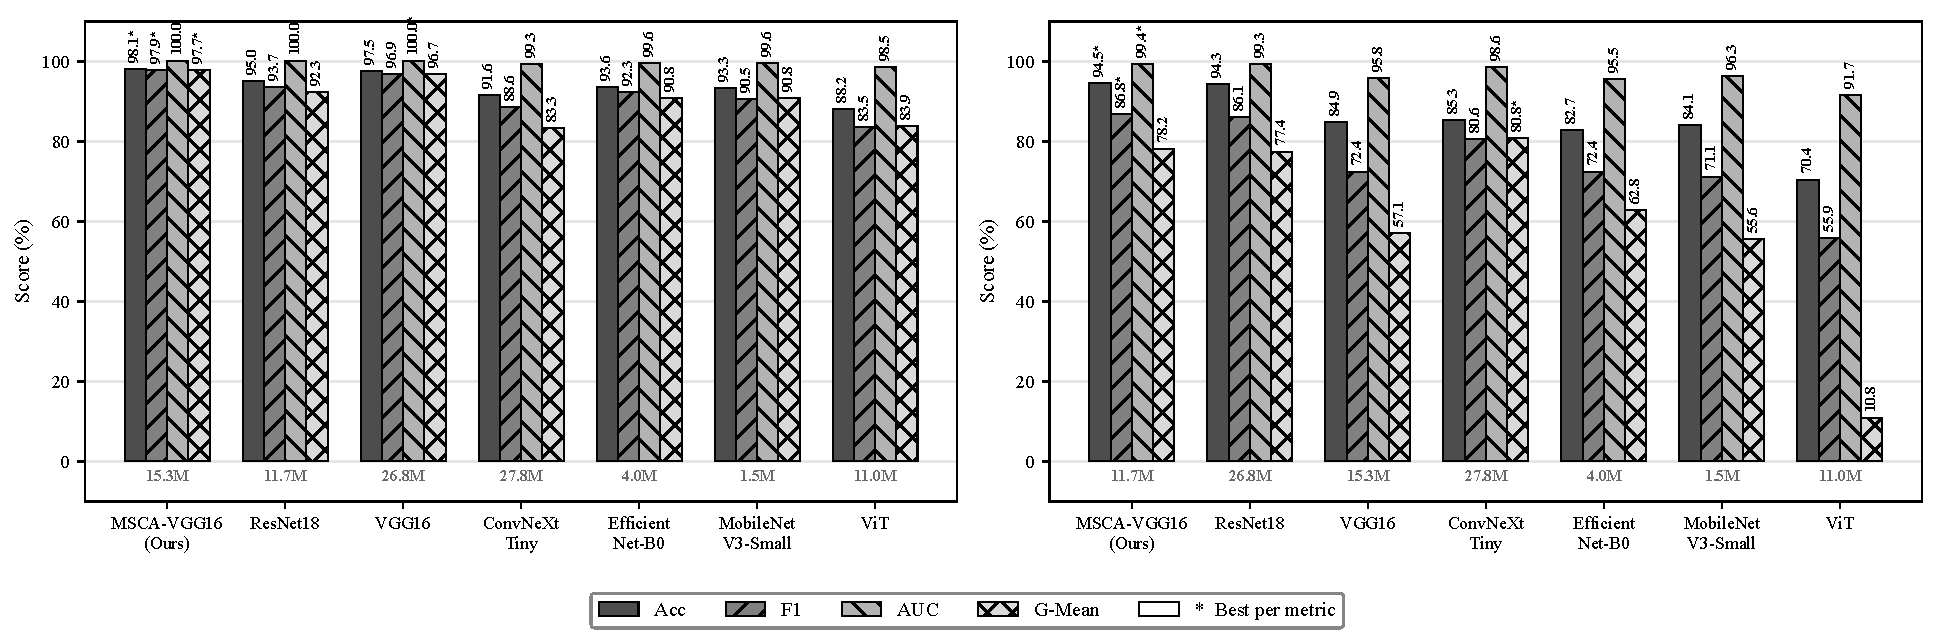
\includegraphics[width=\linewidth]{figures/generalization/generalization_trial_seed42.pdf}
	\caption{Generalization validation across seven backbone networks on the CWRU 12k FE (left) and 48k DE (right) datasets. Best per metric marked with an asterisk. MSCA-VGG16 achieves the highest or competitive scores across all metrics on both datasets, with the most pronounced advantages in F1-score and G-mean under cross-sampling-rate conditions.}
	\label{fig:generalization}
\end{figure*}

\subsection{Noise Robustness Evaluation}
\label{sec:noise_robustness}

To evaluate model robustness under realistic industrial conditions, zero-mean additive Gaussian noise is injected at SNR levels from 5.0 to 30.0~dB. Fig.~\ref{fig:noise_robustness} presents the accuracy, $F_1$-score, and AUC of each backbone network across SNR levels.

The proposed MSCA-VGG16 achieves 100.0\% accuracy at 20.0~dB and above, and retains 91.2\% at the most challenging 5.0~dB level, corresponding to a degradation of only 8.8\% across the full SNR range---the flattest profile among all evaluated networks. This substantially outperforms VGG16 (15.4\%) and EfficientNet-B0 (11.2\%), which suffer near-complete performance collapse at 5.0~dB. This resilience is attributed to the multi-scale channel attention mechanism, which dynamically suppresses noise-dominated frequency bands while preserving fault-discriminative spectral components.

ConvNeXt-Tiny achieves moderate noise immunity, with accuracy ranging from 48.6\% at 5.0~dB to 95.0\% at 30.0~dB. ResNet18 offers a strong balance, retaining 76.3\% at 5.0~dB while achieving 96.9\% at 30.0~dB. ViT degrades modestly under noise (from 83.2\% to 72.5\%) despite the lowest peak accuracy (83.2\% at 30.0~dB). These results confirm that MSCA-VGG16 achieves the best balance between peak discriminative performance and noise robustness, making it suitable for practical industrial deployment where signal quality cannot be guaranteed.

% % Auto-generated from data-optimization/noise_robustness/noise_robustness.csv
\begin{table*}[!htbp]
    \centering
    \caption{Noise Robustness Comparison --- Accuracy (\%) at Different SNR Levels Under Additive Gaussian Noise.}
    \label{tab:noise_robustness}
    \renewcommand{\arraystretch}{1.1}
    \footnotesize
    \setlength{\tabcolsep}{4pt}
    \begin{tabular}{lcccccc}
        \toprule
        \textbf{Model} & $\mathbf{5.0}$~dB & $\mathbf{10.0}$~dB & $\mathbf{15.0}$~dB & $\mathbf{20.0}$~dB & $\mathbf{25.0}$~dB & $\mathbf{30.0}$~dB \\
        \midrule
        \textbf{MSCA-VGG16 (Ours)} & $\mathbf{91.19}$ & $\mathbf{97.45}$ & $\mathbf{99.87}$ & $\mathbf{100.00}$ & $\mathbf{100.00}$ & $\mathbf{100.00}$ \\
        ResNet18 & $76.31$ & $94.78$ & $97.26$ & $97.06$ & $97.06$ & $96.93$ \\
        ConvNeXt-Tiny & $48.56$ & $93.21$ & $94.13$ & $94.84$ & $95.04$ & $95.04$ \\
        EfficientNet-B0 & $11.23$ & $87.01$ & $94.97$ & $95.63$ & $95.37$ & $95.43$ \\
        MobileNetV3-Small & $45.76$ & $85.12$ & $95.76$ & $95.89$ & $95.37$ & $95.43$ \\
        VGG16 & $15.40$ & $78.85$ & $98.02$ & $98.87$ & $98.87$ & $98.87$ \\
        ViT & $72.52$ & $81.92$ & $82.57$ & $83.22$ & $83.03$ & $83.16$ \\
        \bottomrule
    \end{tabular}
\end{table*}


\subsection{Generalization Validation}
\label{sec:generalization}


% % Auto-generated by scripts/analyze_results_three.py
% Date: 2026-06-29 14:57:57

\begin{table*}[!htbp]
    \centering
    \caption{Performance Comparison Across Three CWRU Datasets and Seven Backbone Networks (Mean $\pm$ Std over 3 Independent Trials).}
    \label{tab:three_trial_summary}
    \renewcommand{\arraystretch}{1.1}
    \footnotesize
    \setlength{\tabcolsep}{3.5pt}
    \begin{tabular}{lccccccccc}
        \toprule
        \multirow{2}{*}{\textbf{Model}} & \multicolumn{3}{c}{CWRU 12k DE} & \multicolumn{3}{c}{CWRU 12k FE} & \multicolumn{3}{c}{CWRU 48k DE} \\
         & Acc & F1 & FPR & Acc & F1 & FPR & Acc & F1 & FPR \\
        \midrule
        \textbf{MSCA-VGG16} & $93.26 \pm 2.27$ & $90.38 \pm 3.37$ & $8.76 \pm 2.95$ & $90.75 \pm 0.68$ & $87.25 \pm 1.38$ & $10.54 \pm 0.78$ & $\mathbf{90.25} \pm 1.19$ & $\mathbf{80.45} \pm 1.60$ & $16.36 \pm 0.81$ \\
        ConvNeXt-Tiny & $85.25 \pm 3.09$ & $78.11 \pm 3.74$ & $\mathbf{19.16} \pm 4.03$ & $\mathbf{92.50} \pm 1.39$ & $\mathbf{91.25} \pm 1.75$ & $8.79 \pm 1.79$ & $78.51 \pm 1.85$ & $66.22 \pm 2.99$ & $\mathbf{30.79} \pm 4.13$ \\
        EfficientNet-B0 & $90.56 \pm 2.82$ & $86.40 \pm 4.41$ & $12.26 \pm 3.67$ & $88.58 \pm 2.21$ & $84.32 \pm 2.43$ & $13.02 \pm 2.52$ & $83.03 \pm 3.18$ & $71.54 \pm 3.69$ & $24.85 \pm 5.12$ \\
        MobileNetV3-S & $89.80 \pm 0.56$ & $85.69 \pm 0.76$ & $13.25 \pm 0.72$ & $87.56 \pm 1.72$ & $83.14 \pm 1.78$ & $14.19 \pm 1.96$ & $84.34 \pm 0.72$ & $73.33 \pm 0.83$ & $22.90 \pm 0.92$ \\
        ResNet18 & $\mathbf{94.71} \pm 1.76$ & $\mathbf{92.46} \pm 2.83$ & $6.86 \pm 2.28$ & $91.15 \pm 0.92$ & $87.73 \pm 1.83$ & $10.09 \pm 1.05$ & $85.50 \pm 0.06$ & $74.60 \pm 0.39$ & $21.35 \pm 1.02$ \\
        VGG16 & $93.93 \pm 0.85$ & $90.60 \pm 1.35$ & $7.88 \pm 1.11$ & $91.50 \pm 0.89$ & $89.20 \pm 1.11$ & $9.69 \pm 1.02$ & $89.84 \pm 2.26$ & $79.77 \pm 2.58$ & $16.64 \pm 1.60$ \\
        ViT & $91.73 \pm 1.98$ & $88.88 \pm 2.79$ & $10.74 \pm 2.57$ & $86.31 \pm 3.71$ & $80.15 \pm 7.21$ & $\mathbf{16.23} \pm 4.60$ & $85.61 \pm 0.45$ & $75.57 \pm 0.80$ & $22.27 \pm 0.58$ \\
        \bottomrule
    \end{tabular}
\end{table*}


To assess generalization beyond the primary benchmark, experiments are conducted on the 12k FE dataset and the 48k DE dataset. The same AW-DPCNN pipeline and MSCA-VGG16 classifier are applied without architectural modifications, with only the signal-processing parameters adjusted per Section~\ref{sec:dataset_preprocessing} to maintain consistent temporal duration and frequency resolution. Key findings are summarized as follows.

\textbf{1) Cross-sensor generalization (12k FE).} The proposed MSCA-VGG16 achieves the highest accuracy (97.45\%) and F1-score (97.01\%) on the fan-end dataset, outperforming ResNet18 (95.08\%) and VGG16 (95.33\%). This confirms that the multi-scale channel attention mechanism transfers effectively across sensor positions, with the dynamic channel recalibration suppressing sensor-specific noise patterns while preserving fault-discriminative spectral features.

\textbf{2) Cross-sampling-rate generalization (48k DE).} MSCA-VGG16 again achieves the best accuracy (94.81\%), followed closely by ResNet18 (94.21\%). VGG16 degrades substantially (89.46\%), and the lightweight architectures (MobileNetV3-Small, 78.29\%; EfficientNet-B0, 79.00\%) suffer severe performance collapse. This pattern demonstrates that the multi-scale branches in MSCA-VGG16 are particularly beneficial at higher sampling rates, simultaneously capturing fine-grained high-frequency fault signatures and broader spectral patterns.

\textbf{3) Architecture robustness ranking.} Across both generalization datasets, the performance ranking is consistent, i.e., MSCA-VGG16 leads, followed by ResNet18 and VGG16, with ConvNeXt-Tiny intermediate (87--92\%), and ViT consistently trailing (69--86\%). The lightweight backbones (MobileNetV3-Small, EfficientNet-B0) are competitive at 12k FE but collapse at 48k DE, indicating that their efficiency-driven design choices limit capacity for complex high-bandwidth spectral modeling.

These results are visualized in Fig.~\ref{fig:generalization}, which compares the per-model performance across both generalization datasets. The figure confirms that MSCA-VGG16 consistently achieves the highest scores across all metrics on both the fan-end and 48 kHz datasets, with particularly pronounced advantages in G-mean and F1-score under the more challenging cross-sampling-rate scenario. These results confirm that MSCA-VGG16 generalizes robustly across sensor positions and sampling rates without dataset-specific tuning, validating its practical applicability under varying data acquisition configurations.

\section{Conclusion}
\label{section5}

This paper has presented a two-stage framework for vibration-based bearing fault diagnosis comprising AW-DPCNN for adaptive multi-representation fusion and MSCA-VGG16 for fused representation classification. AW-DPCNN introduces contrast-guided dynamic weighting, dual-channel representation-specific convolutional stimuli, and iterative pulse-coupled dynamics to adaptively integrate STFT spectrograms with GADF temporal encodings. MSCA-VGG16 augments a VGG16 backbone with multi-scale convolution, squeeze-and-excitation channel attention, and a compact embedding head to exploit the complementary information in the fused representations.

Extensive experiments on the CWRU bearing dataset demonstrate that the full pipeline achieves 99.85\% accuracy on the 12 kHz drive-end primary benchmark, outperforming seven baseline architectures including ResNet18 (98.39\%) and VGG16 (99.19\%). Systematic ablation confirms that AW-DPCNN fusion contributes 2.93\% over single-representation baselines and that multi-scale convolution contributes 0.54\% gain. Representation comparisons across twelve time--frequency and temporal encoding combinations validate STFT with GADF as the optimal input pair (96.30\% accuracy). Noise robustness evaluations at SNR levels from 5.0 to 30.0~dB demonstrate that MSCA-VGG16 maintains discriminative performance under realistic conditions, substantially outperforming competing architectures at low SNR. Cross-sensor generalization to the fan-end position (97.45\%) and cross-sampling-rate generalization to 48 kHz (94.81\%) confirm the robustness of the learned representations without dataset-specific tuning.

These results collectively demonstrate that adaptive multi-representation fusion combined with multi-scale channel attention provides an effective and generalizable approach to non-stationary vibration signal fault diagnosis. Future work will explore several directions: (i) extending the AW-DPCNN framework to multi-sensor fusion, where vibration signals from multiple measurement points are jointly weighted and integrated; (ii) evaluating the proposed pipeline on larger-scale industrial datasets under variable-speed and fluctuating-load conditions; and (iii) investigating lightweight architectures to reduce the computational cost of AW-DPCNN fusion for real-time deployment.


% \begin{table*}[!htbp]
% \centering
% \caption{Noise Robustness Comparison --- Accuracy (\%) at Different SNR Levels.}
% \label{tab:noise_robustness}
% \renewcommand{\arraystretch}{1.1}
% \small
% \begin{tabular}{lccccccc}
% \toprule
% \textbf{Model} & Clean & 5.0~dB & 10.0~dB & 15.0~dB & 20.0~dB & 25.0~dB & 30.0~dB \\
% \midrule
% \textbf{MSCA-VGG16} & 95.1 & 92.9 & 93.9 & 94.7 & 94.8 & 95.1 & 95.2 \\
% VGG16 & 94.7 & 83.5 & 93.7 & 94.5 & 94.6 & 94.8 & 94.7 \\
% ViT & 88.0 & 73.8 & 85.8 & 87.7 & 88.4 & 88.0 & 88.4 \\
% EfficientNet-B0 & 91.0 & 14.1 & 75.3 & 88.4 & 91.0 & 90.8 & 91.3 \\
% MobileNetV3-Small & 84.7 & 56.9 & 72.6 & 83.6 & 84.2 & 84.0 & 84.0 \\
% ConvNeXt-Tiny & 76.4 & 78.5 & 78.0 & 77.0 & 76.4 & 76.7 & 76.4 \\
% \bottomrule
% \end{tabular}
% \end{table*}


% \begin{table*}[!htbp]
% \centering
% \caption{Performance Comparison on the EXP1 Dataset (Seed 42)}
% \label{tab:exp1_comparison}
% \renewcommand{\arraystretch}{1.15}
% \small
% \begin{tabular}{lcccccc}
% \toprule
% \textbf{Network} & \textbf{Acc} & \textbf{F1} & \textbf{G-Mean} & \textbf{AUC} & \textbf{$\kappa$} & \textbf{Params (M)} \\
% \midrule
% \textbf{MSCA-VGG16 (Ours)} & \textbf{95.1} & \textbf{92.9} & \textbf{90.3} & 99.9 & \textbf{94.3} & 26.8 \\
% VGG16 & 94.7 & 91.9 & 89.0 & \textbf{99.9} & 93.8 & 15.3 \\
% EfficientNet-B0 & 91.0 & 86.7 & 83.1 & 98.9 & 89.5 & 4.0 \\
% ViT & 88.0 & 84.1 & 82.3 & 99.2 & 85.9 & 11.0 \\
% MobileNetV3-Small & 84.7 & 79.3 & 75.0 & 98.2 & 82.0 & 1.5 \\
% ConvNeXt-Tiny & 76.4 & 66.0 & 45.1 & 97.1 & 72.3 & 27.8 \\
% \bottomrule
% \end{tabular}
% \end{table*}

% \begin{table*}[!htbp]
% \centering
% \caption{Training Summary and Leakage Check}
% \label{tab:exp1_training}
% \renewcommand{\arraystretch}{1.15}
% \small
% \begin{tabular}{lccccc}
% \toprule
% \textbf{Network} & \textbf{Best Epoch} & \textbf{Val F1} & \textbf{Params (M)} & \textbf{FLOPs (M)} & \textbf{Shuffled Acc} \\
% \midrule
% \textbf{MSCA-VGG16 (Ours)} & 24 & 99.8 & 26.8 & 15947 & 15.7 \\
% VGG16 & 30 & 99.8 & 15.3 & 15394 & 15.6 \\
% EfficientNet-B0 & 14 & 92.0 & 4.0 & 15338 & 15.7 \\
% ViT & 29 & 78.8 & 11.0 & 65 & 15.5 \\
% MobileNetV3-Small & 30 & 84.3 & 1.5 & 1845 & 15.8 \\
% ConvNeXt-Tiny & 18 & 95.3 & 27.8 & 25708 & 15.5 \\
% \bottomrule
% \end{tabular}
% \end{table*}

% \begin{figure*}[!htbp]
% 	\centering
% 	\begin{subfigure}{0.32\textwidth}
% 		\centering
% 		\includegraphics[width=\linewidth]{../experiments/experiment_result/exp1/convnext_tiny/exp1_convnext_tiny/trial_seed42/figures/confusion_matrix.png}
% 		\caption{ConvNeXt-Tiny}
% 	\end{subfigure}
% 	\hfill
% 	\begin{subfigure}{0.32\textwidth}
% 		\centering
% 		\includegraphics[width=\linewidth]{../experiments/experiment_result/exp1/vit/exp1_vit/trial_seed42/figures/confusion_matrix.png}
% 		\caption{ViT}
% 	\end{subfigure}
% 	\hfill
% 	\begin{subfigure}{0.32\textwidth}
% 		\centering
% 		\includegraphics[width=\linewidth]{../experiments/experiment_result/exp1/vgg16/exp1_vgg16/trial_seed42/figures/confusion_matrix.png}
% 		\caption{VGG16}
% 	\end{subfigure}

% 	\vspace{3mm}

% 	\begin{subfigure}{0.32\textwidth}
% 		\centering
% 		\includegraphics[width=\linewidth]{../experiments/experiment_result/exp1/efficientnet_b0/exp1_efficientnet_b0/trial_seed42/figures/confusion_matrix.png}
% 		\caption{EfficientNet-B0}
% 	\end{subfigure}
% 	\hfill
% 	\begin{subfigure}{0.32\textwidth}
% 		\centering
% 		\includegraphics[width=\linewidth]{../experiments/experiment_result/exp1/mobilenetv3_small/exp1_mobilenetv3_small/trial_seed42/figures/confusion_matrix.png}
% 		\caption{MobileNetV3-Small}
% 	\end{subfigure}
% 	\hfill
% 	\begin{subfigure}{0.32\textwidth}
% 		\centering
% 		\includegraphics[width=\linewidth]{../experiments/experiment_result/exp1/MSCA_VGG16/exp1_MSCA_VGG16/trial_seed42/figures/confusion_matrix.png}
% 		\caption{MSCA-VGG16 (Ours)}
% 	\end{subfigure}
% 	\caption{t-SNE feature visualization of different backbone networks on the transformer acoustic test set. The proposed MSCA-VGG16 produces the most compact and well-separated clusters, indicating superior discriminative representation learning.}
% 	\label{fig:tsne_backbones}
% \end{figure*}


% % Auto-generated by scripts/plot_roc_all.py
% Date: 2026-06-29 11:34:44

\begin{table*}[!htbp]
    \centering
    \caption{Per-Class AUC Values Across Backbone Networks.}
    \label{tab:roc_auc}
    \renewcommand{\arraystretch}{1.05}
    \footnotesize
    \begin{tabular}{lccccccc}
        \toprule
        \textbf{Fault Class} & \textbf{MSCA-VGG16 (Ours)} & ConvNeXt-Tiny & EfficientNet-B0 & MobileNetV3-Small & ResNet18 & VGG16 & ViT \\
        \midrule
        BF007 & $\mathbf{1.000}$ & $0.954$ & $0.948$ & $0.969$ & $0.982$ & $0.999$ & $0.990$ \\
        BF014 & $\mathbf{1.000}$ & $0.997$ & $1.000$ & $1.000$ & $1.000$ & $1.000$ & $0.998$ \\
        BF021 & $0.997$ & $0.974$ & $0.971$ & $0.970$ & $\mathbf{1.000}$ & $0.998$ & $0.998$ \\
        IF007 & $\mathbf{1.000}$ & $1.000$ & $1.000$ & $1.000$ & $1.000$ & $1.000$ & $0.999$ \\
        IF014 & $\mathbf{0.927}$ & $0.665$ & $0.650$ & $0.723$ & $0.622$ & $0.738$ & $0.696$ \\
        IF021 & $\mathbf{1.000}$ & $1.000$ & $0.992$ & $0.995$ & $1.000$ & $1.000$ & $0.998$ \\
        Normal & $\mathbf{1.000}$ & $1.000$ & $1.000$ & $1.000$ & $1.000$ & $1.000$ & $1.000$ \\
        OF007 & $\mathbf{1.000}$ & $1.000$ & $1.000$ & $1.000$ & $1.000$ & $1.000$ & $1.000$ \\
        OF014 & $0.981$ & $0.872$ & $0.919$ & $0.939$ & $0.946$ & $\mathbf{0.982}$ & $0.941$ \\
        OF021 & $\mathbf{1.000}$ & $1.000$ & $0.998$ & $1.000$ & $1.000$ & $1.000$ & $1.000$ \\
        \midrule
        \textbf{Macro} & $\mathbf{0.990}$ & $0.946$ & $0.948$ & $0.959$ & $0.955$ & $0.971$ & $0.962$ \\
        \textbf{Micro} & $\mathbf{0.995}$ & $0.975$ & $0.983$ & $0.988$ & $0.988$ & $0.994$ & $0.986$ \\
        \bottomrule
    \end{tabular}
\end{table*}







% \begin{figure*}[!htbp] 
% \centering
% 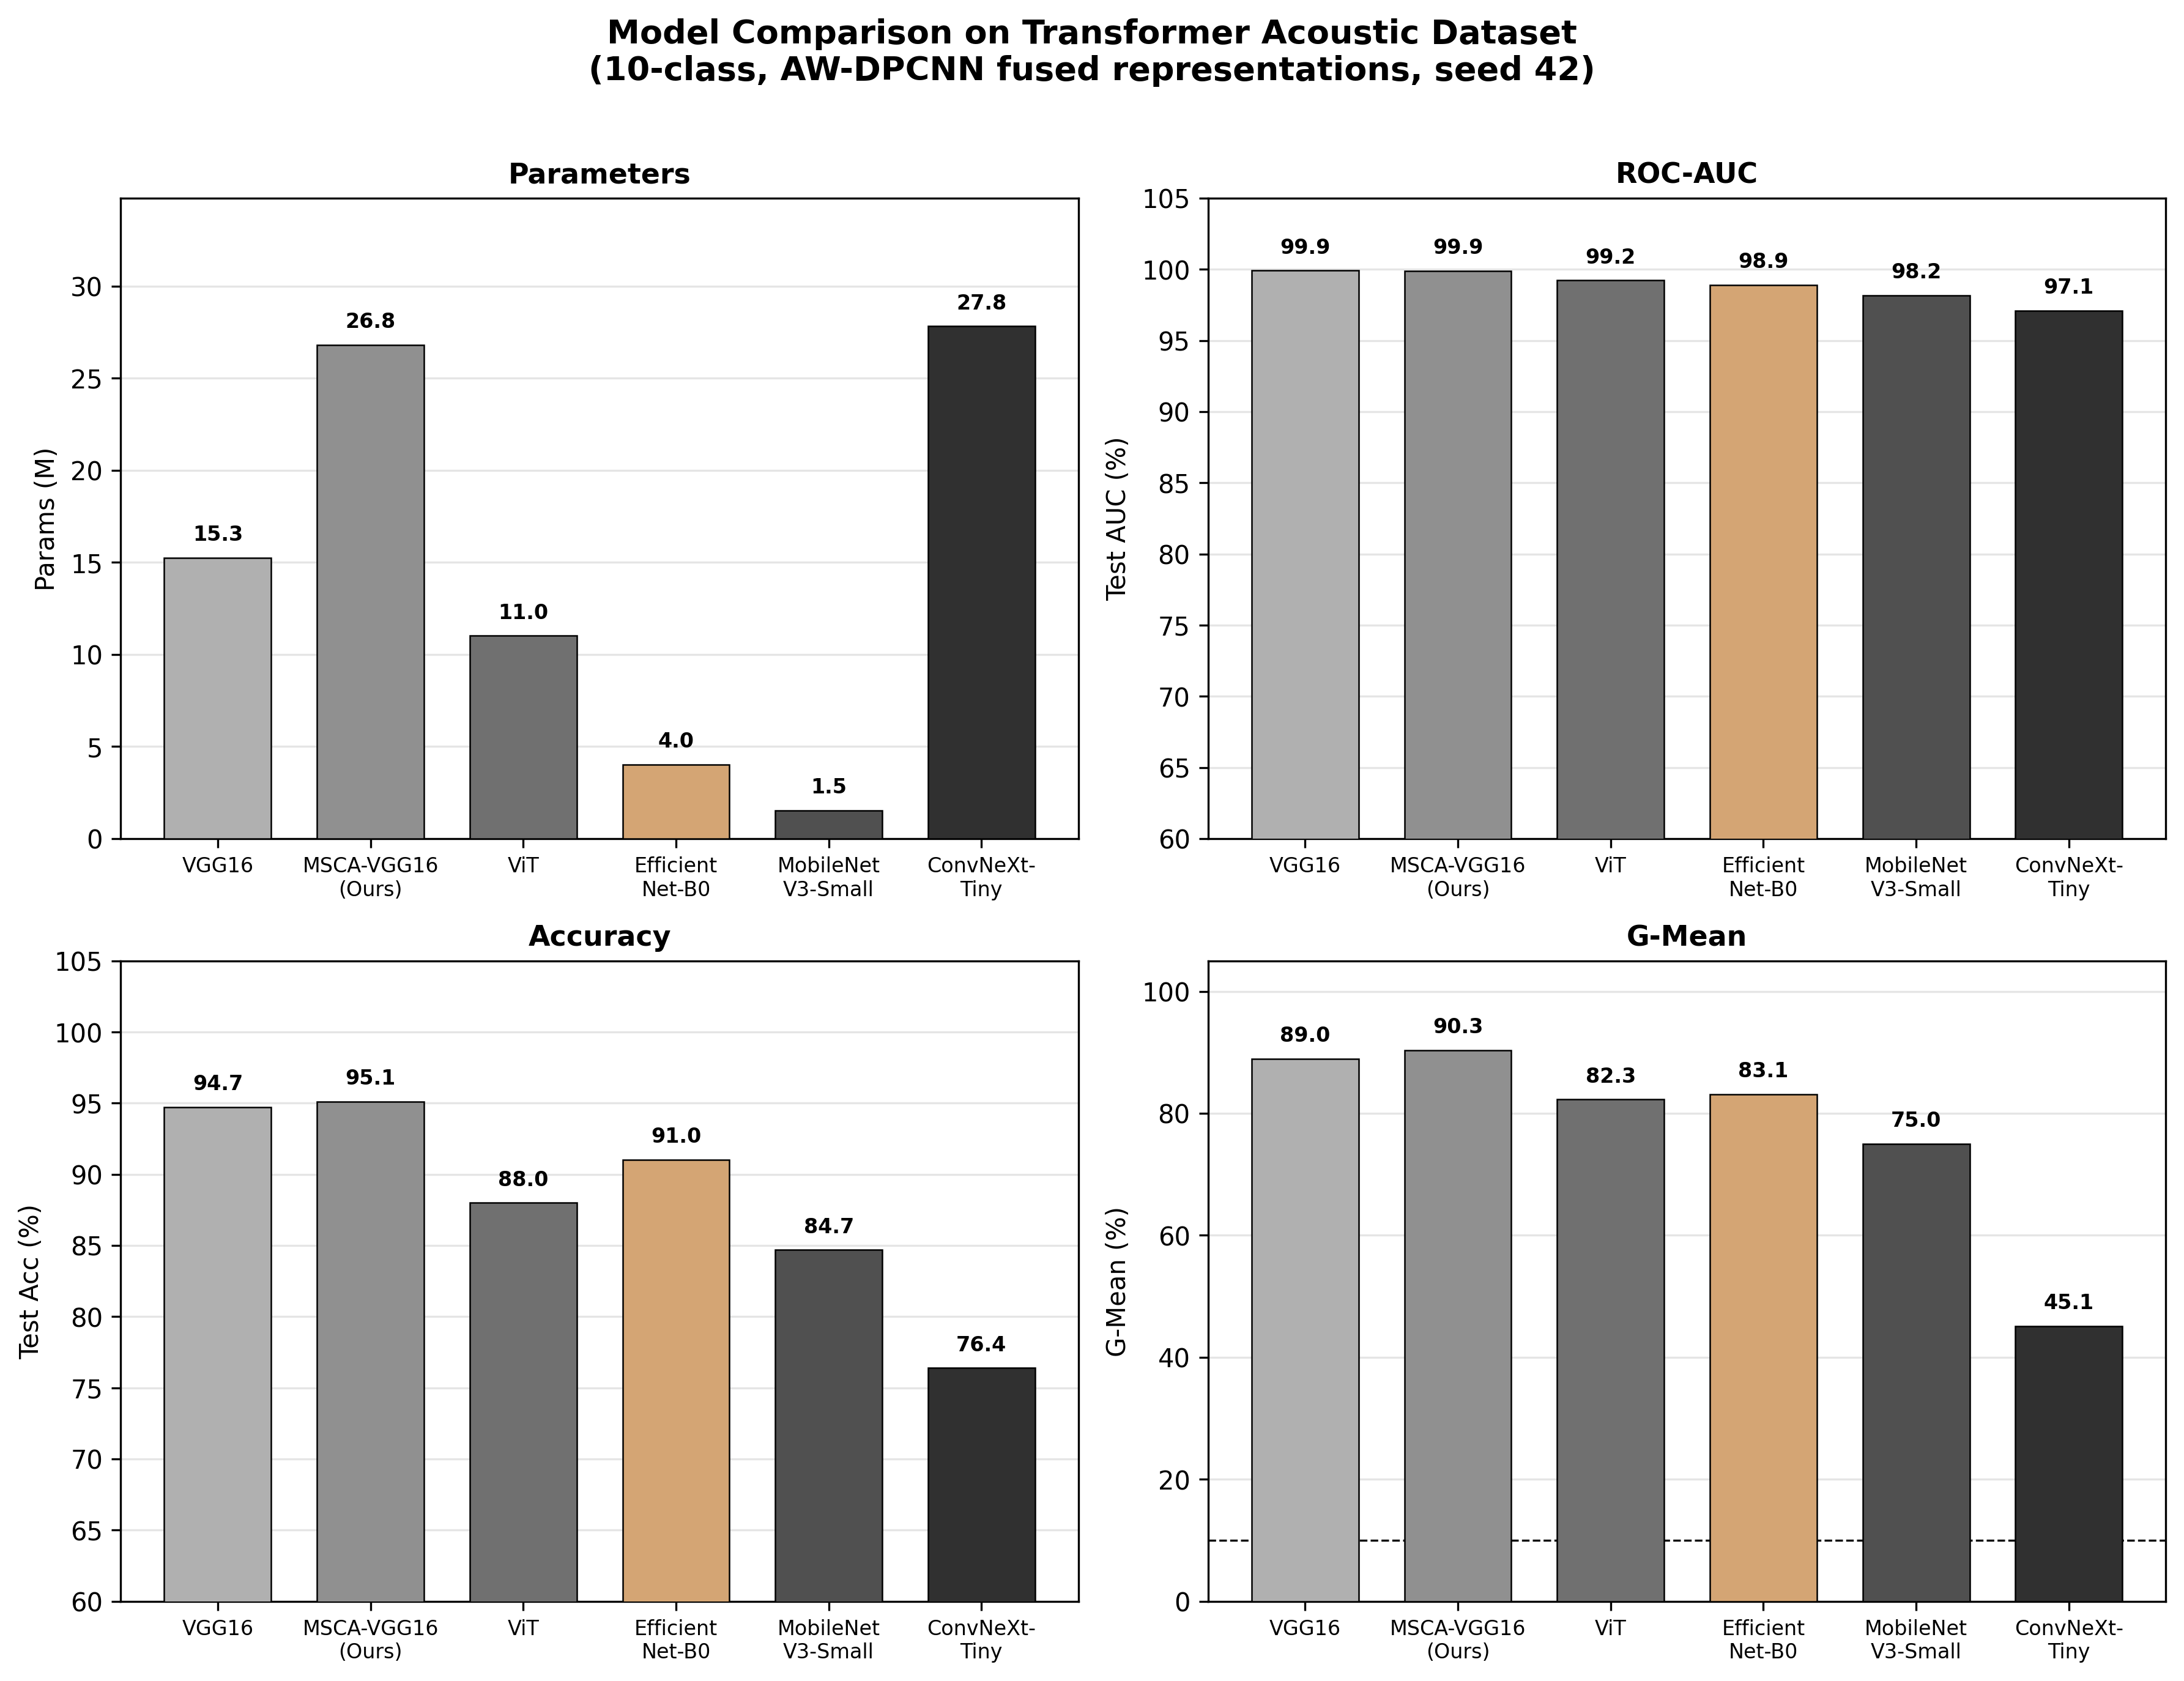
\includegraphics[width=\linewidth]{../paper/figures/model_comparison_panel.png}
% \caption{}
% \label{}
% \end{figure*}





% % Auto-generated from data-optimization/noise_robustness/noise_robustness.csv
\begin{table*}[!htbp]
    \centering
    \caption{Noise Robustness Comparison --- Accuracy (\%) at Different SNR Levels Under Additive Gaussian Noise.}
    \label{tab:noise_robustness}
    \renewcommand{\arraystretch}{1.1}
    \footnotesize
    \setlength{\tabcolsep}{4pt}
    \begin{tabular}{lcccccc}
        \toprule
        \textbf{Model} & $\mathbf{5.0}$~dB & $\mathbf{10.0}$~dB & $\mathbf{15.0}$~dB & $\mathbf{20.0}$~dB & $\mathbf{25.0}$~dB & $\mathbf{30.0}$~dB \\
        \midrule
        \textbf{MSCA-VGG16 (Ours)} & $\mathbf{91.19}$ & $\mathbf{97.45}$ & $\mathbf{99.87}$ & $\mathbf{100.00}$ & $\mathbf{100.00}$ & $\mathbf{100.00}$ \\
        ResNet18 & $76.31$ & $94.78$ & $97.26$ & $97.06$ & $97.06$ & $96.93$ \\
        ConvNeXt-Tiny & $48.56$ & $93.21$ & $94.13$ & $94.84$ & $95.04$ & $95.04$ \\
        EfficientNet-B0 & $11.23$ & $87.01$ & $94.97$ & $95.63$ & $95.37$ & $95.43$ \\
        MobileNetV3-Small & $45.76$ & $85.12$ & $95.76$ & $95.89$ & $95.37$ & $95.43$ \\
        VGG16 & $15.40$ & $78.85$ & $98.02$ & $98.87$ & $98.87$ & $98.87$ \\
        ViT & $72.52$ & $81.92$ & $82.57$ & $83.22$ & $83.03$ & $83.16$ \\
        \bottomrule
    \end{tabular}
\end{table*}



% \begin{figure*}[!htbp] 
% \centering
% 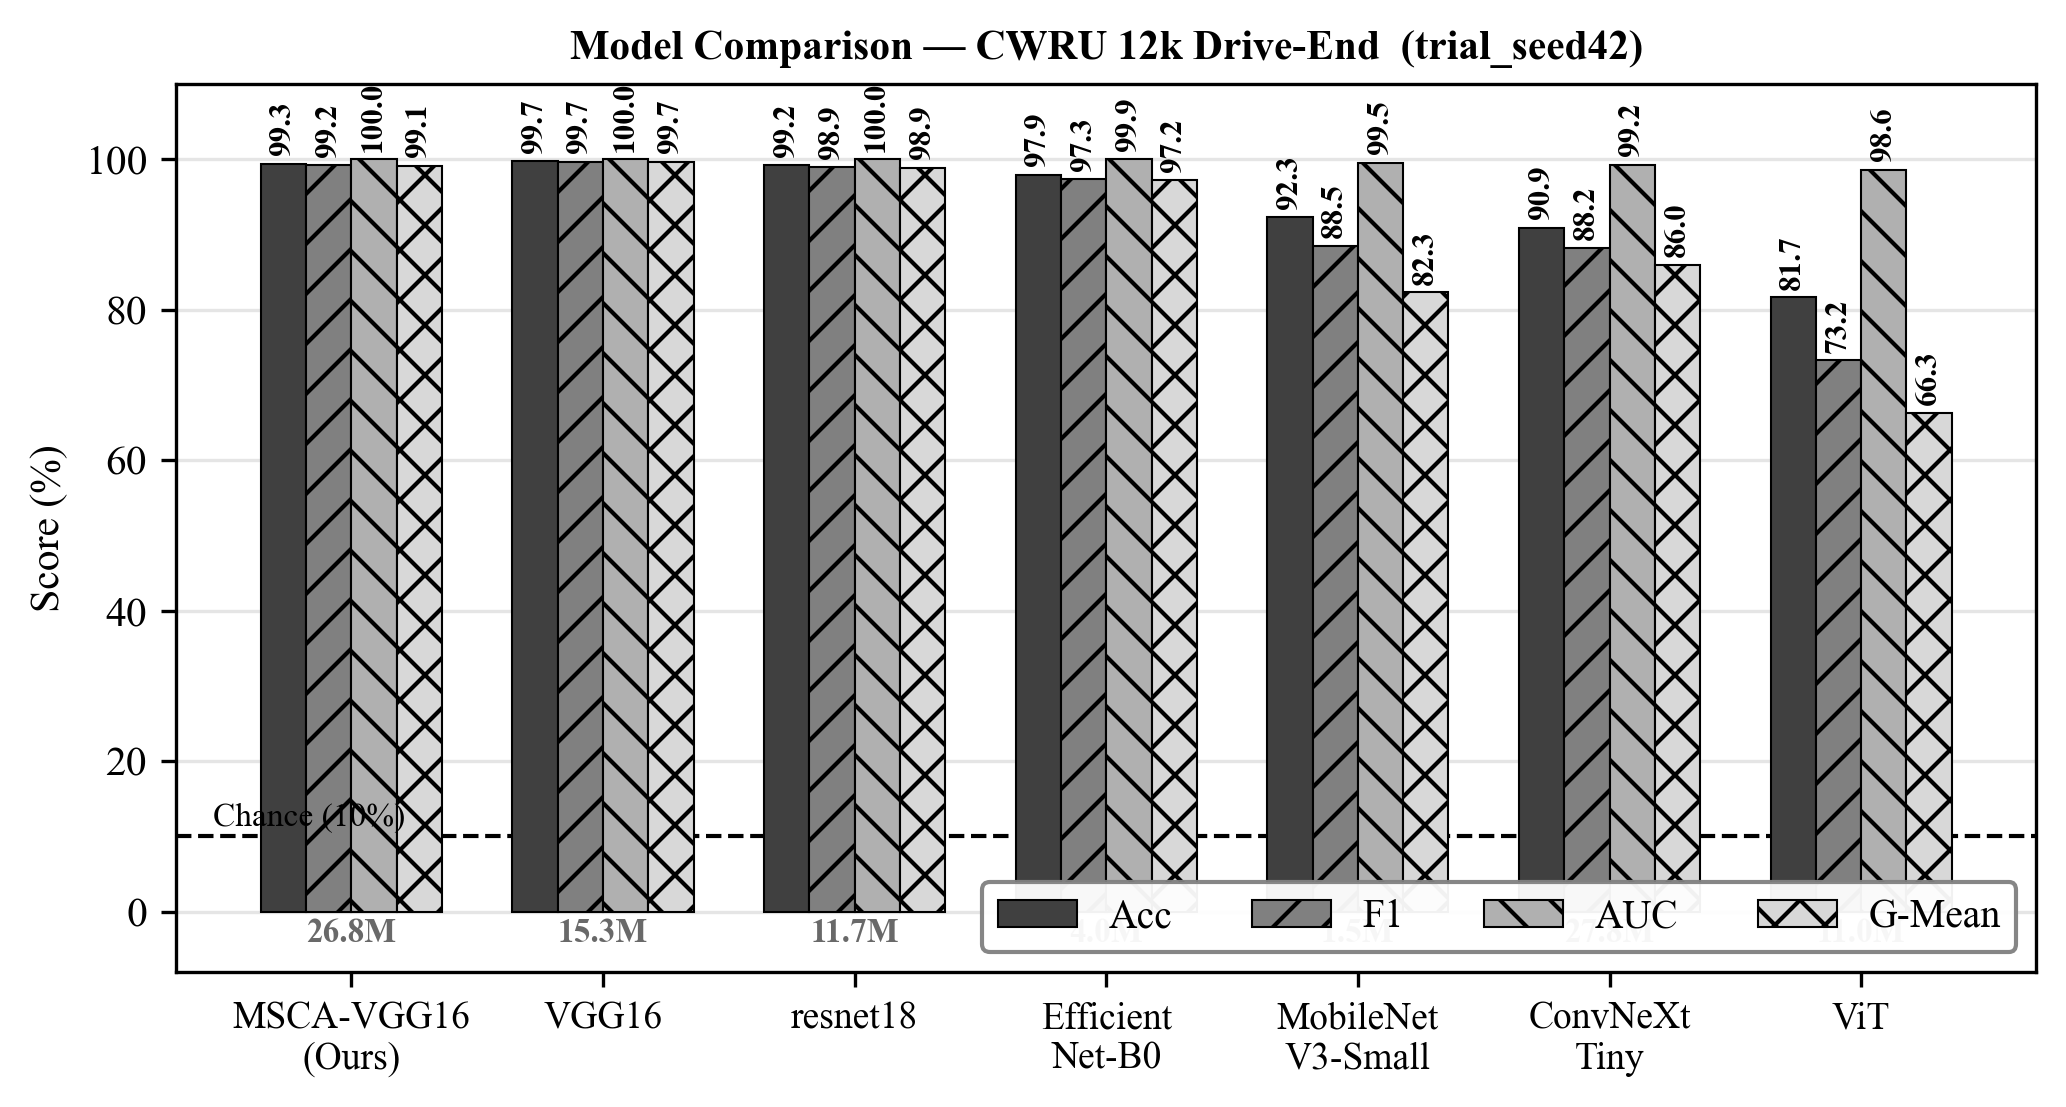
\includegraphics[width=\linewidth]{figures/model_comparison/model_comparison_12k_de_trial_seed42.png}
% \caption{}
% \label{}
% \end{figure*}


% The overall architecture of the proposed MSCA-VGG16 network is illustrated in Fig.~\ref{MSCA-VGG}.
% \begin{figure*}[!htbp]
% 	\centering
% 	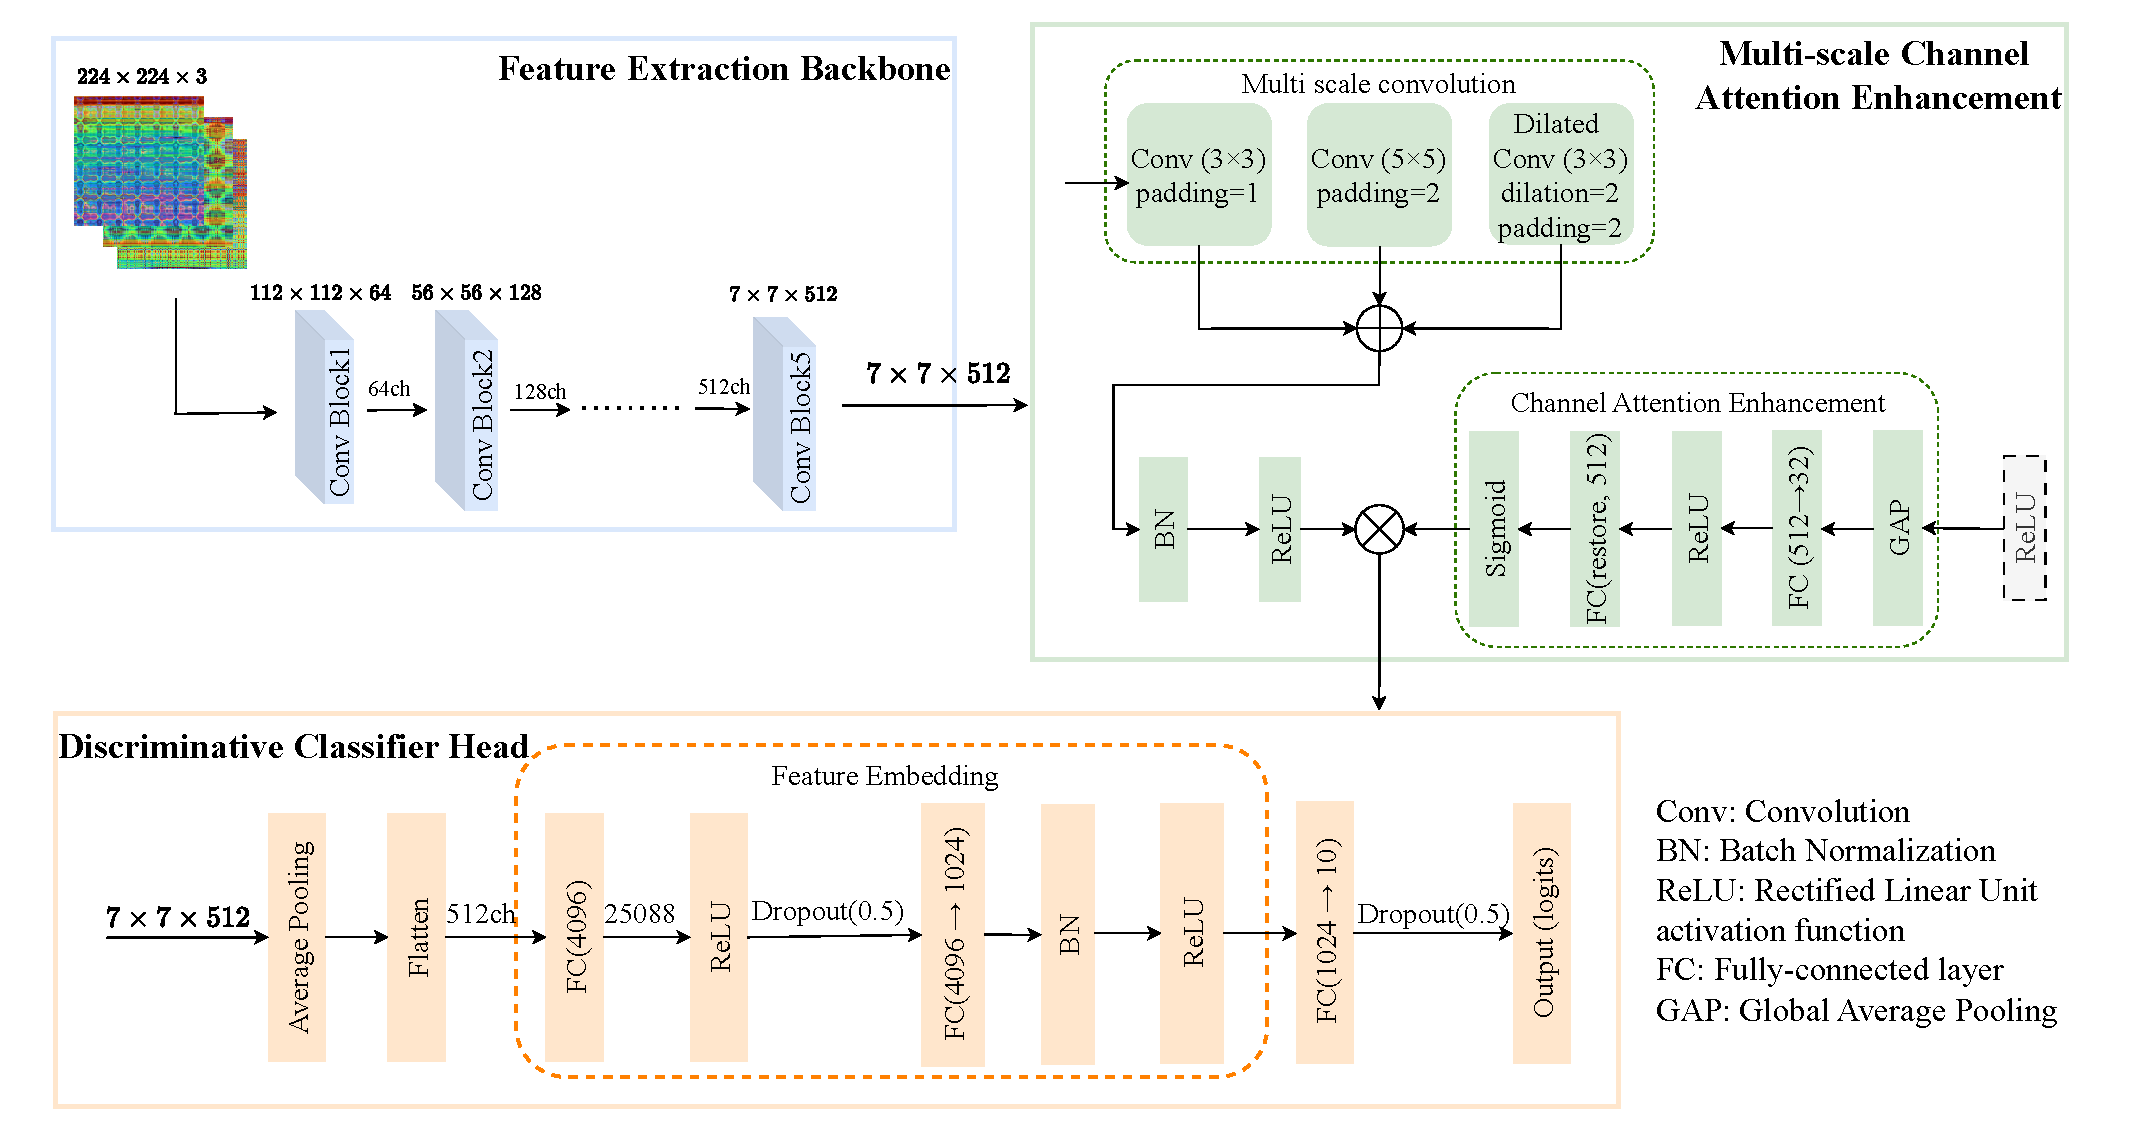
\includegraphics[width=\textwidth]{MSCA-VGG16/MSCA-VGG16}
% 	\caption{Overall architecture of the proposed MSCA-VGG16 network. The fused AW-DPCNN image is processed by a convolutional backbone, followed by a multi-scale convolution module, squeeze-and-excitation channel attention, and a compact embedding head for fault classification.}
% 	\label{MSCA-VGG}
% \end{figure*}


% \balance

\bibliographystyle{IEEEtran}
\bibliography{references}

\end{document}